
\section{3 lepton training for bump search testing}\label{sec:3lep}


To better accertain and map the usefulness of the regular and variational autoencoder in the search for 
new physics, two MonteCarlo signals were used as test cases. They both are 3 lep +$e_T^{miss}$ final state SUSY signals,
and thus are fit to use for testing. The two autoencoders will be tested on four metrics. 
\begin{itemize}
    \item Low reconstruction error on SM MC
    \item Background to signal ratio in $e_T^{miss}$ signal region
    \item Possible resonance in trilepton signal region
    \item Significance search in $e_T^{miss}$ signal region
\end{itemize}



\subsubsection*{Regular autoencoder output}

Below are the reconstruction error distributions for the two signals for both the shallow and deep 
regular autoencoder.

\begin{figure}[H]
    \centering
    \begin{subfigure}{.49\textwidth}
        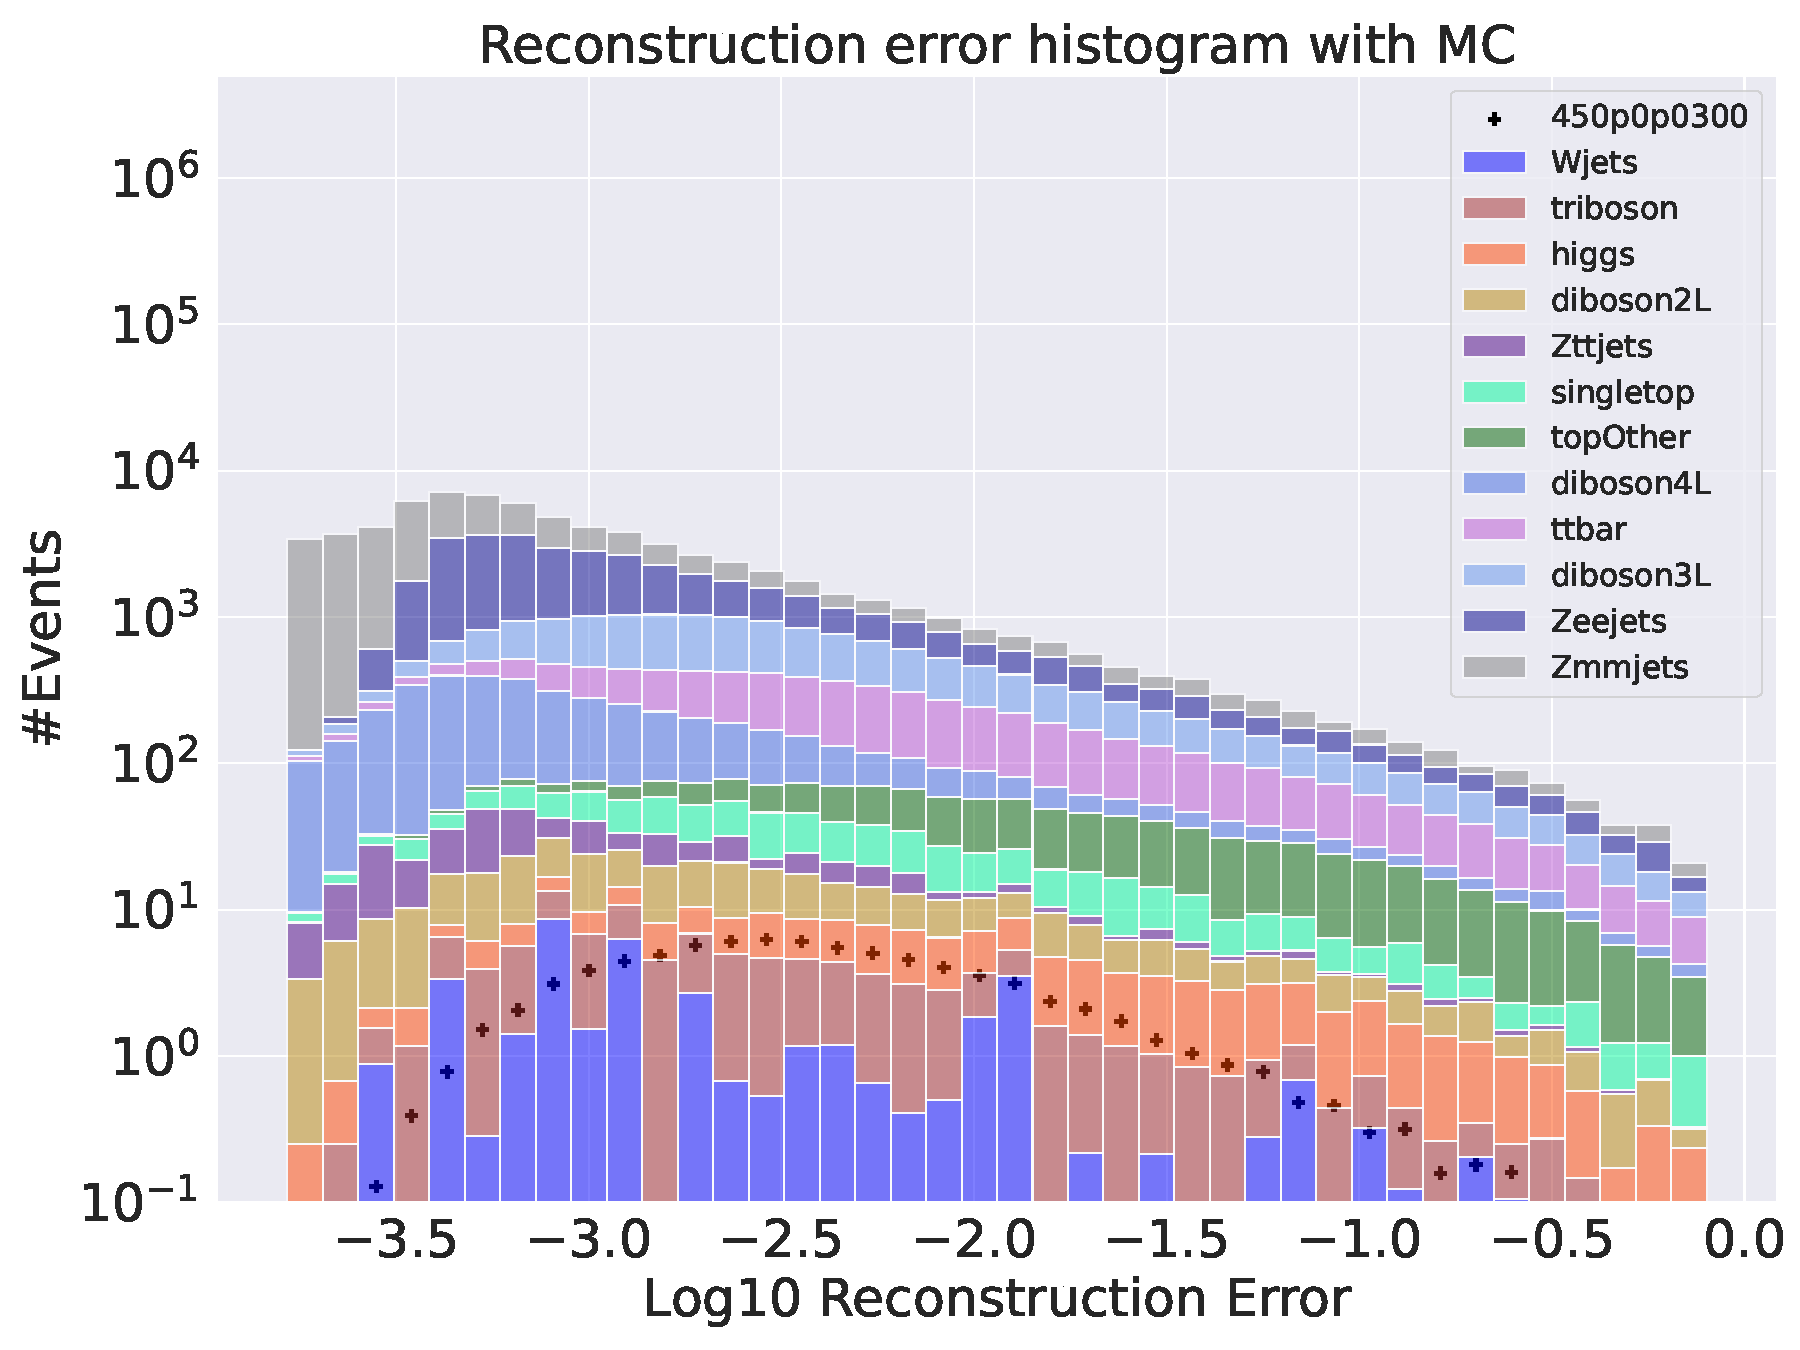
\includegraphics[width=\textwidth]{Figures/AE_testing/big/3lep/b_data_recon_big_rm3_feats_sig_450p0p0300.pdf}
        \caption{ }
        \label{fig:AE_3lep_big_450}
    \end{subfigure}
    \hfill
    \begin{subfigure}{.49\textwidth}
        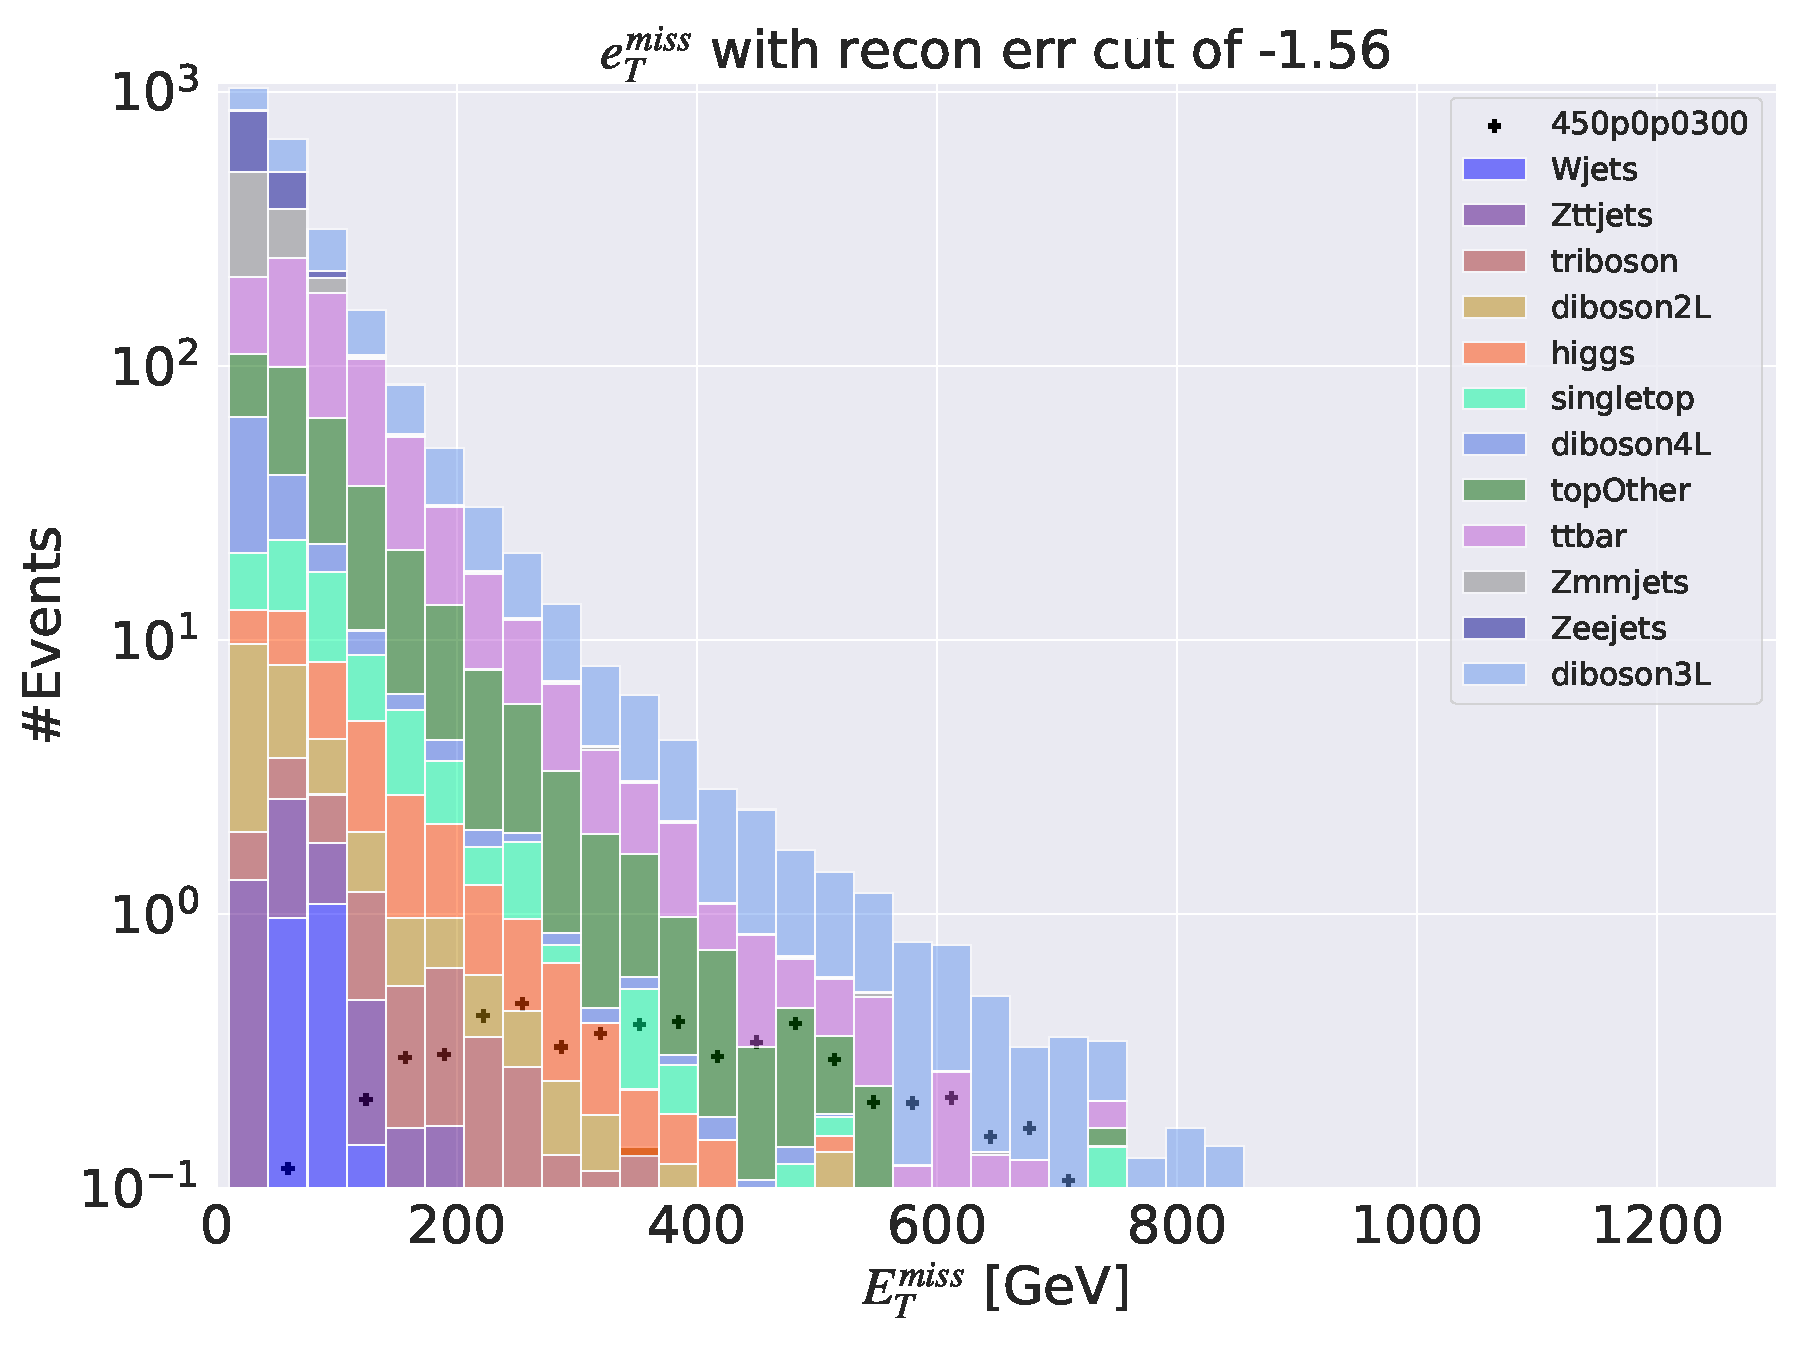
\includegraphics[width=\textwidth]{Figures/AE_testing/big/3lep/b_data_recon_big_rm3_feats_sig_450p0p0300_etmiss_recon_errcut_-1.56.pdf}
        \caption{}
        \label{fig:AE_3lep_big_etmiss_450}
    \end{subfigure}
    \hfill
    \begin{subfigure}{.49\textwidth}
        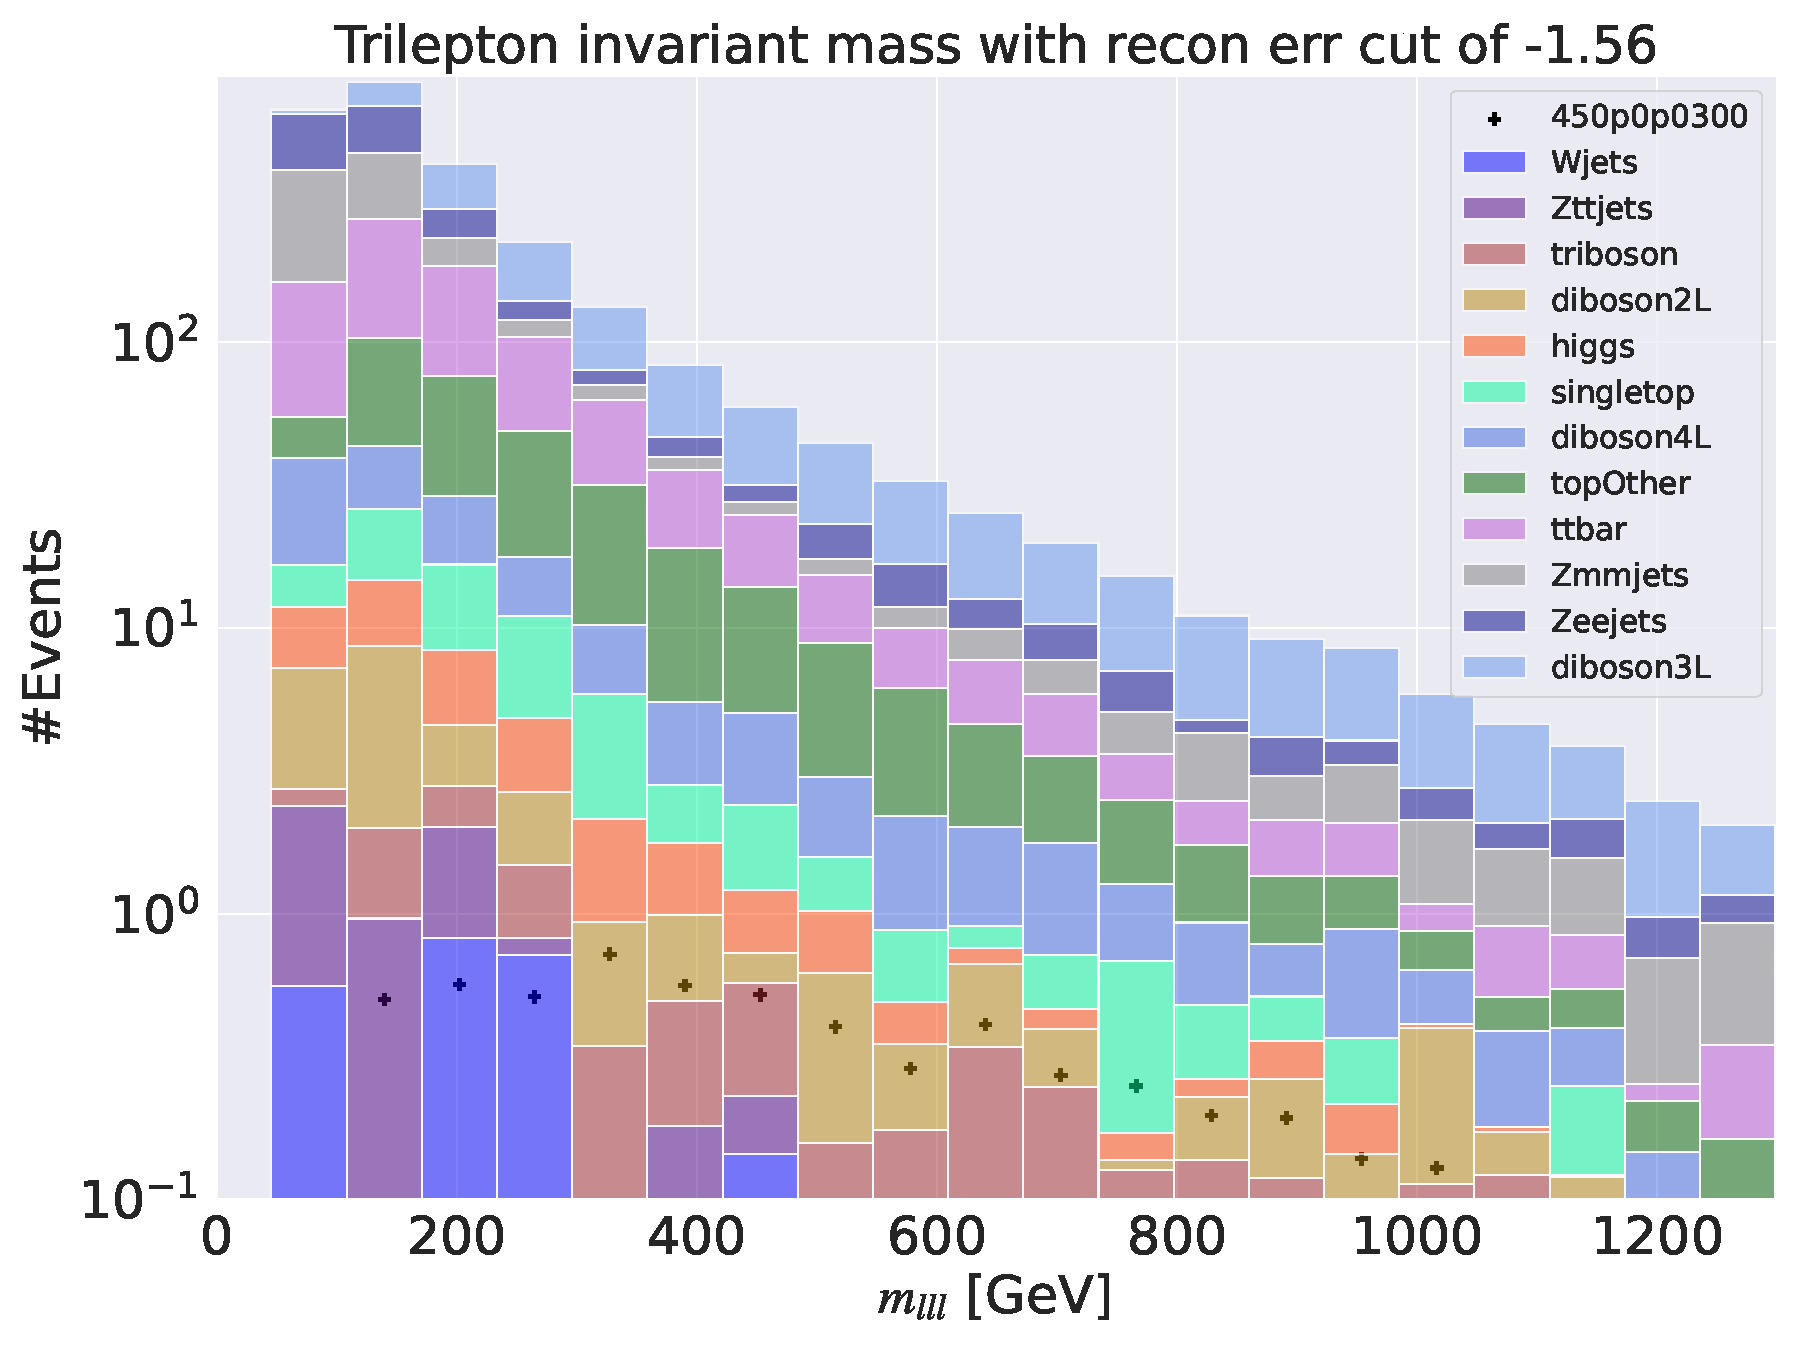
\includegraphics[width=\textwidth]{Figures/AE_testing/big/3lep/b_data_recon_big_rm3_feats_sig_450p0p0300_mlll_recon_errcut_-1.56.pdf}
        \caption{}
        \label{fig:AE_3lep_big_mlll_450}
    \end{subfigure}
    \hfill   
    \begin{subfigure}{.49\textwidth}
        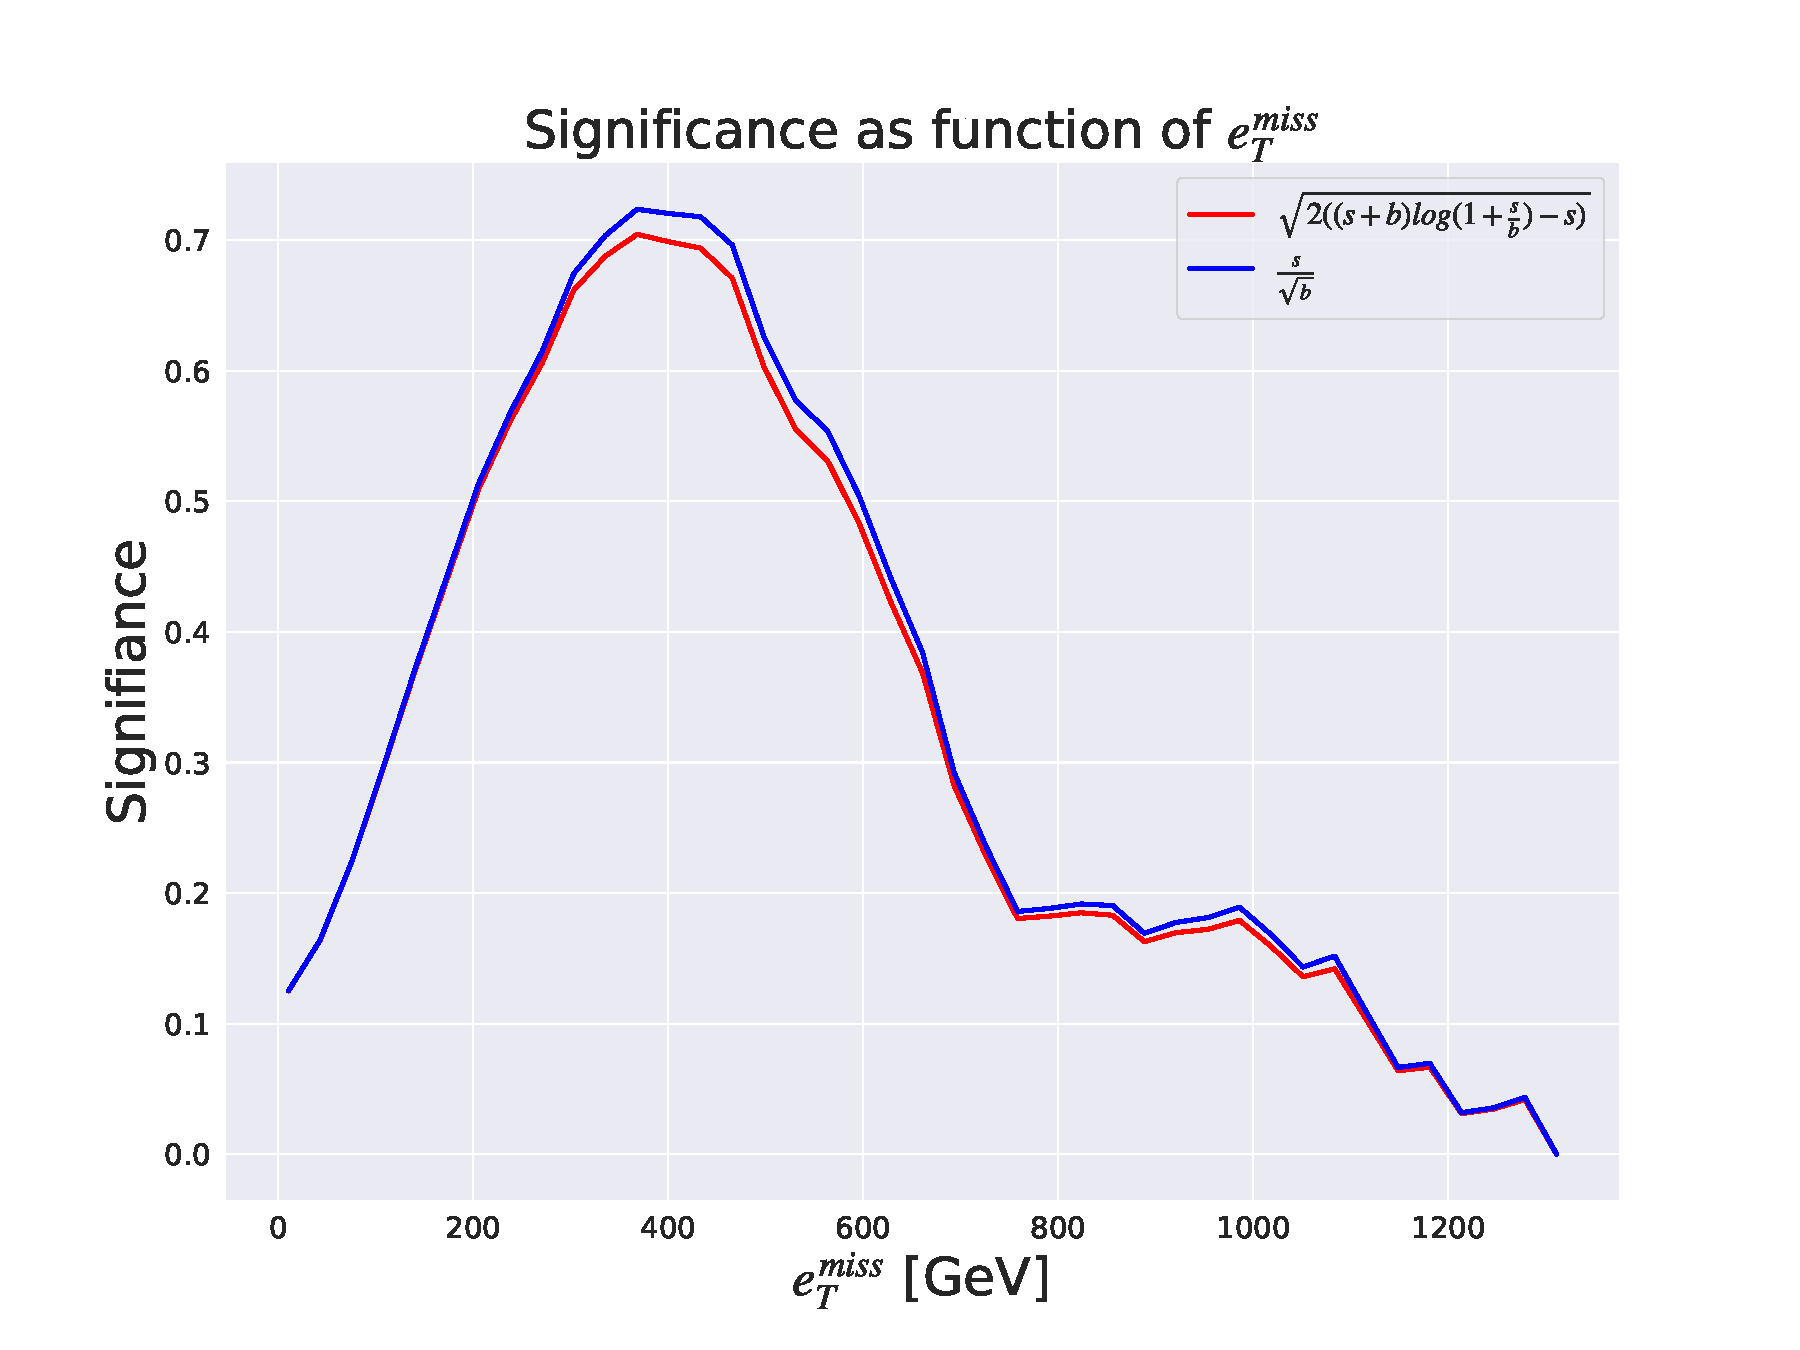
\includegraphics[width=\textwidth]{Figures/AE_testing/big/3lep/significance_etmiss_450p0p0300_-1.5648275418402864.pdf}
        \caption{}
        \label{fig:AE_3lep_big_signi_450}
    \end{subfigure}
    \hfill      
    \caption[3lep deep network | $450p300$ | AE]{Reconstruction error, $e_T^{miss}$ signal region, $m_{lll}$ signal region and significance as function of 
    $e_T^{miss}$ for the deep regular autoencoder using the SUSY $450p300$.}
    \label{fig:AE_3lep_big_rec_sig_signi_450}
\end{figure}

\begin{figure}[H]
    \centering
    \begin{subfigure}{.49\textwidth}
        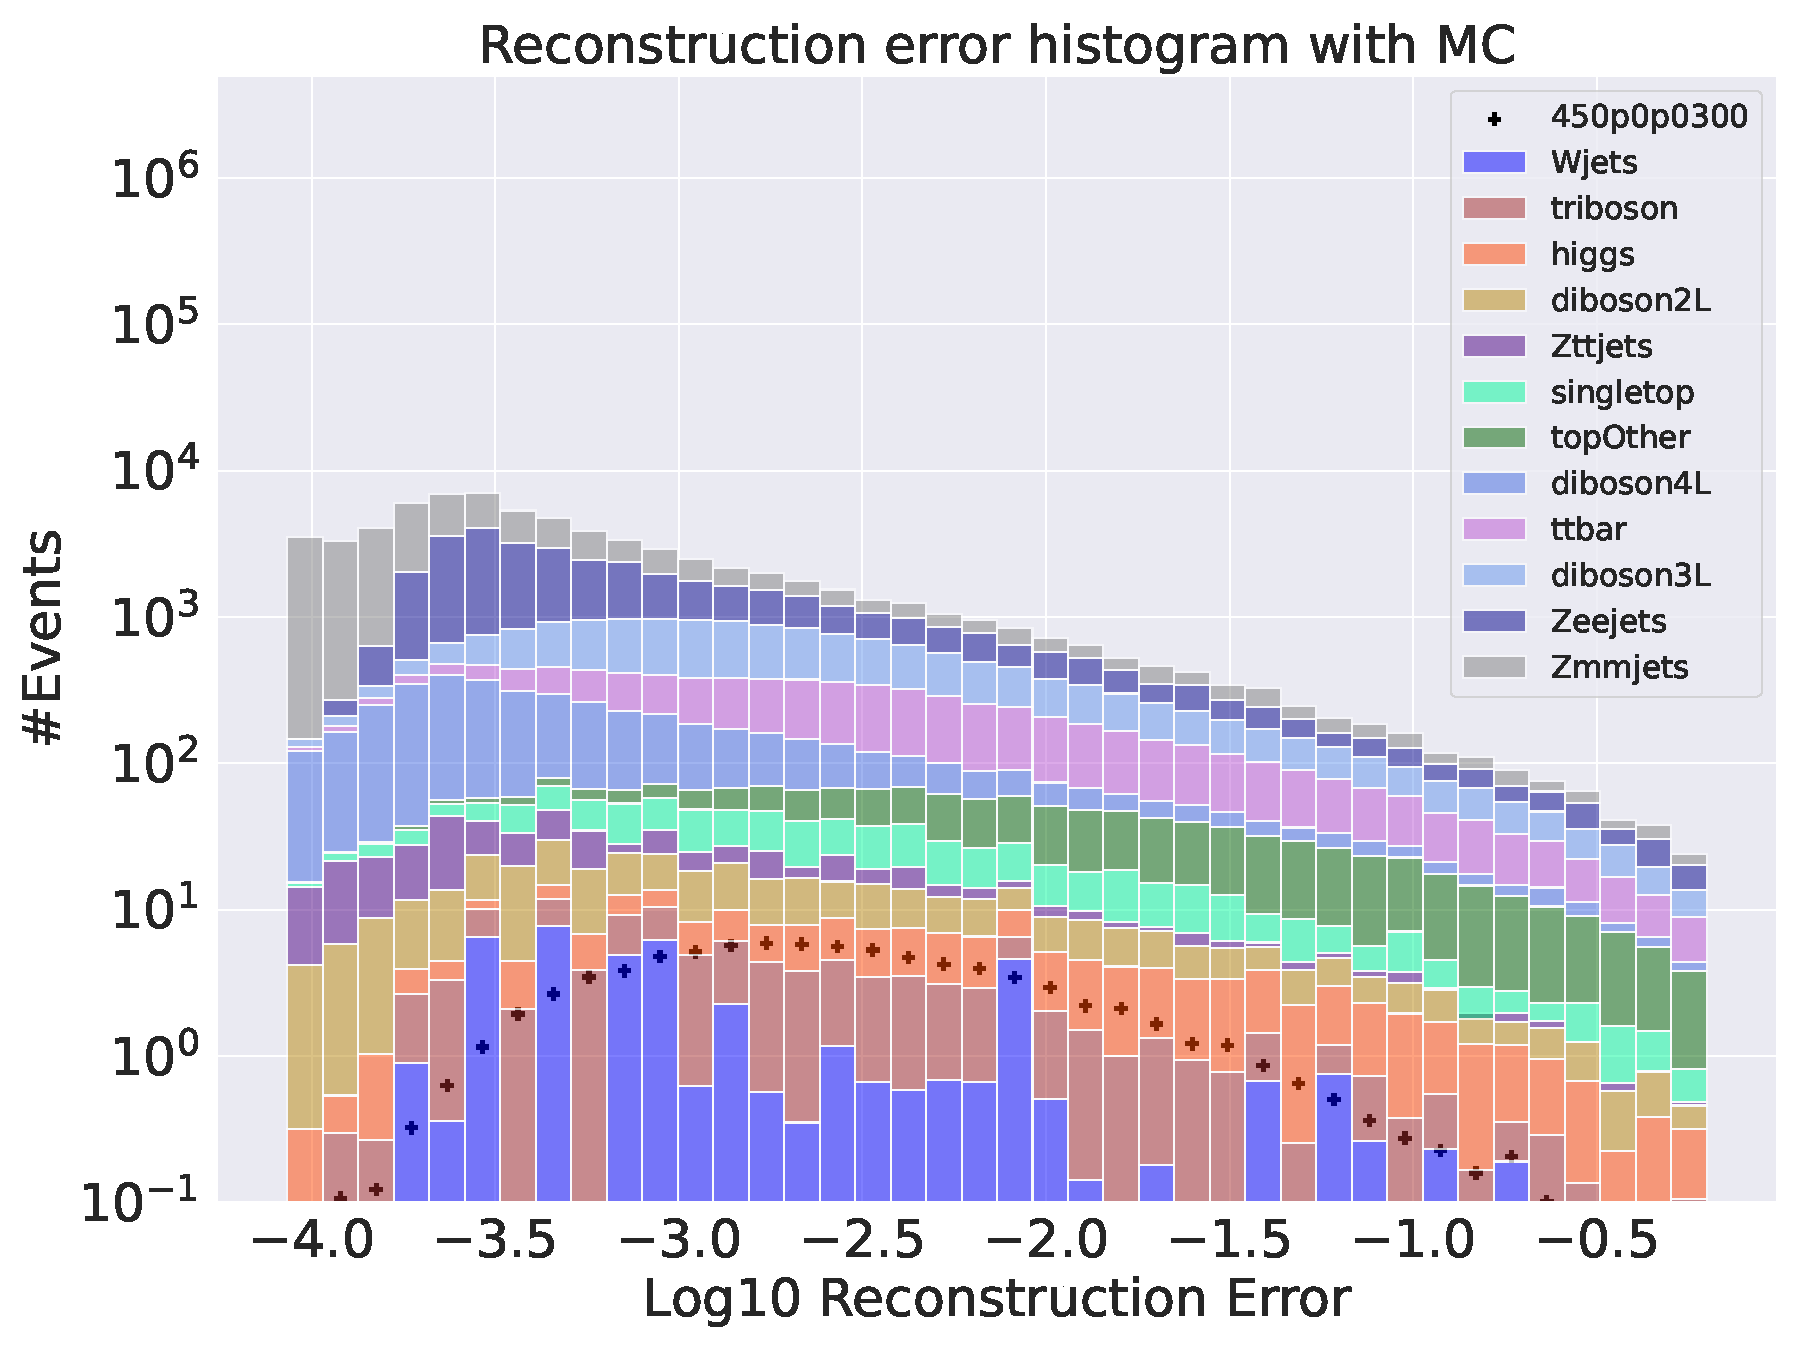
\includegraphics[width=\textwidth]{Figures/AE_testing/small/3lep/b_data_recon_big_rm3_feats_sig_450p0p0300.pdf}
        \caption{ }
        \label{fig:AE_3lep_small_450}
    \end{subfigure}
    \hfill
    \begin{subfigure}{.49\textwidth}
        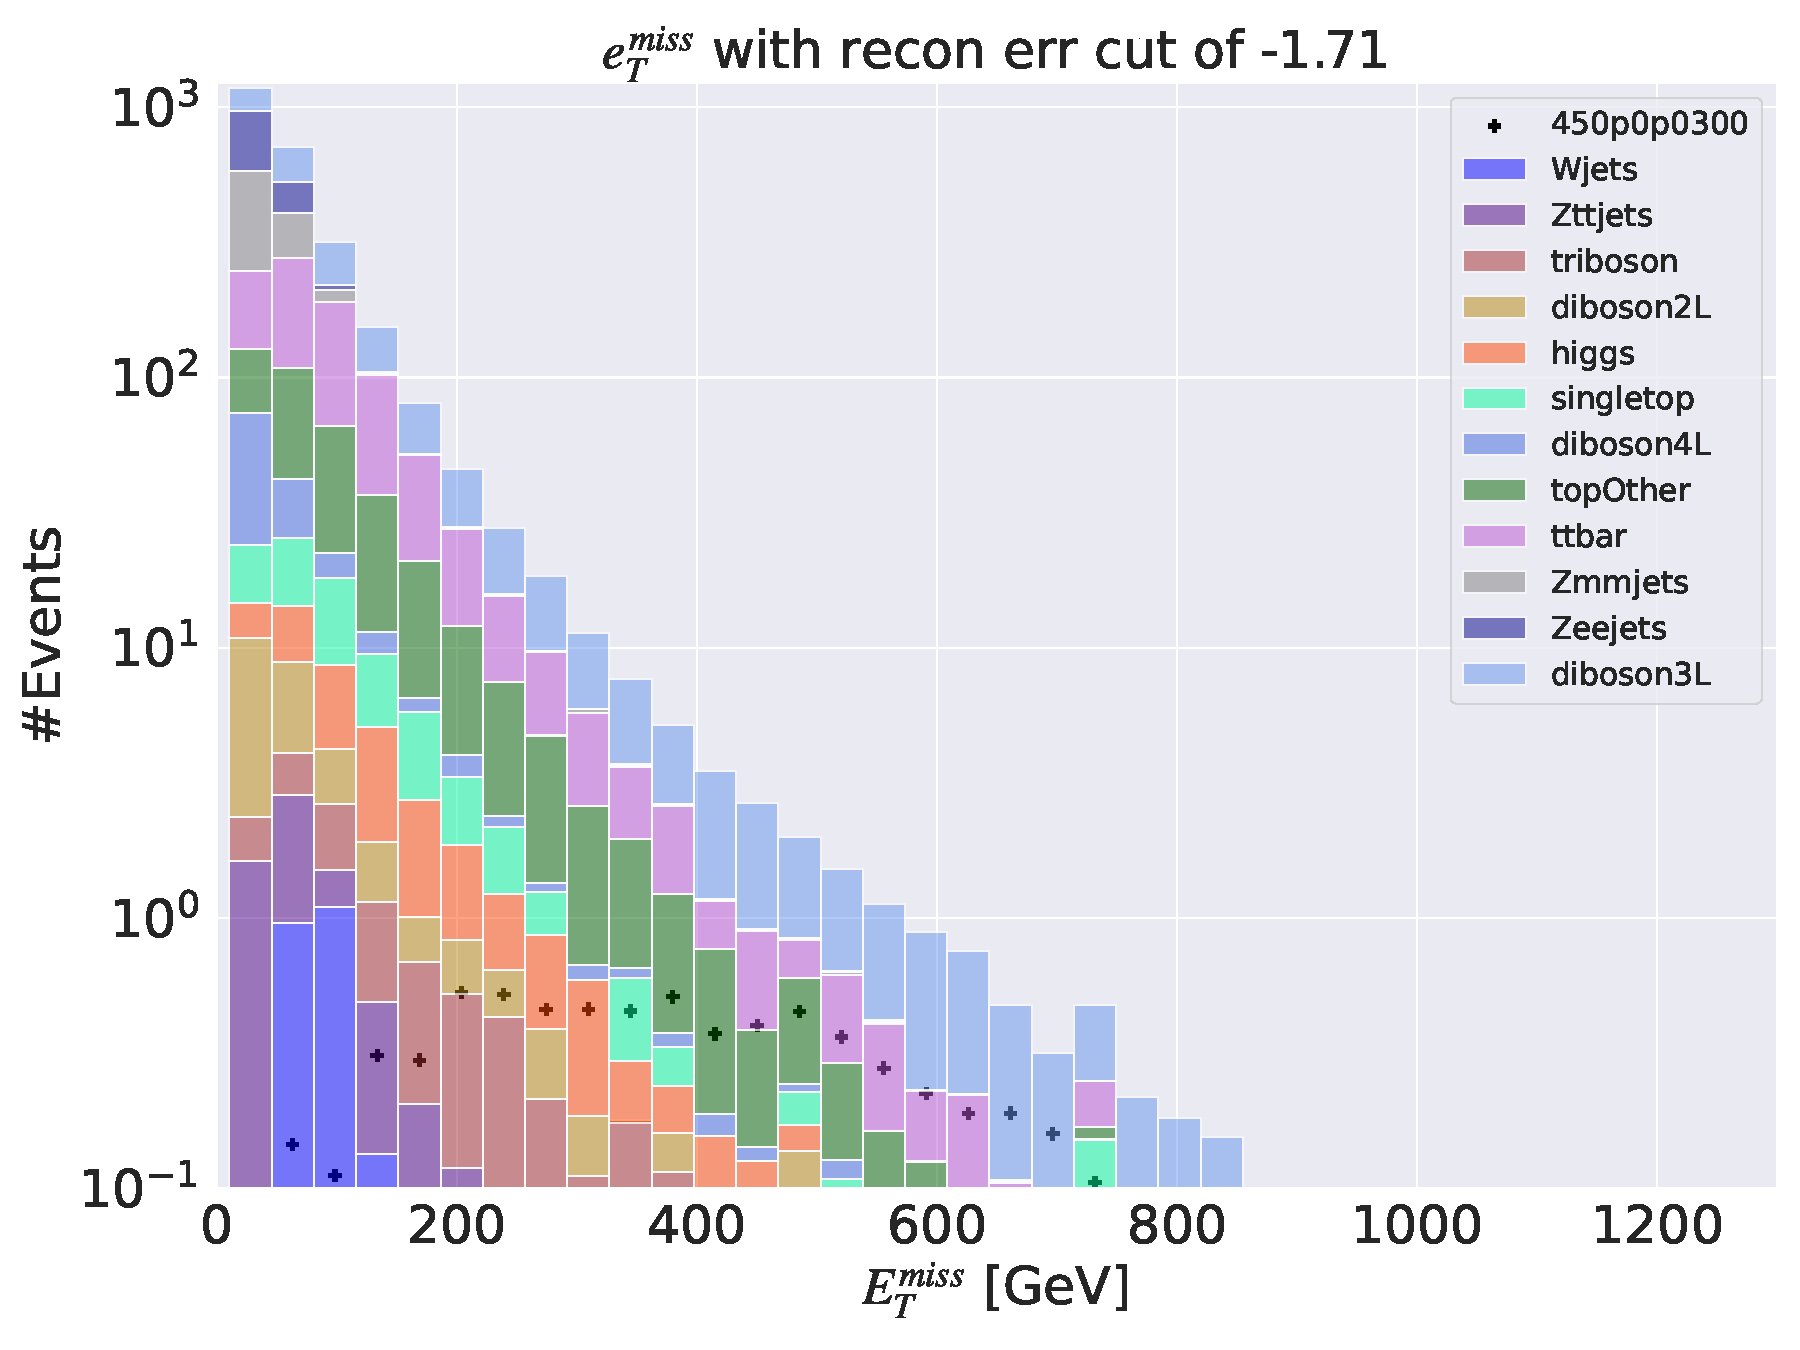
\includegraphics[width=\textwidth]{Figures/AE_testing/small/3lep/b_data_recon_big_rm3_feats_sig_450p0p0300_etmiss_recon_errcut_-1.71.pdf}
        \caption{}
        \label{fig:AE_3lep_small_etmiss_450}
    \end{subfigure}
    \hfill
    \begin{subfigure}{.49\textwidth}
        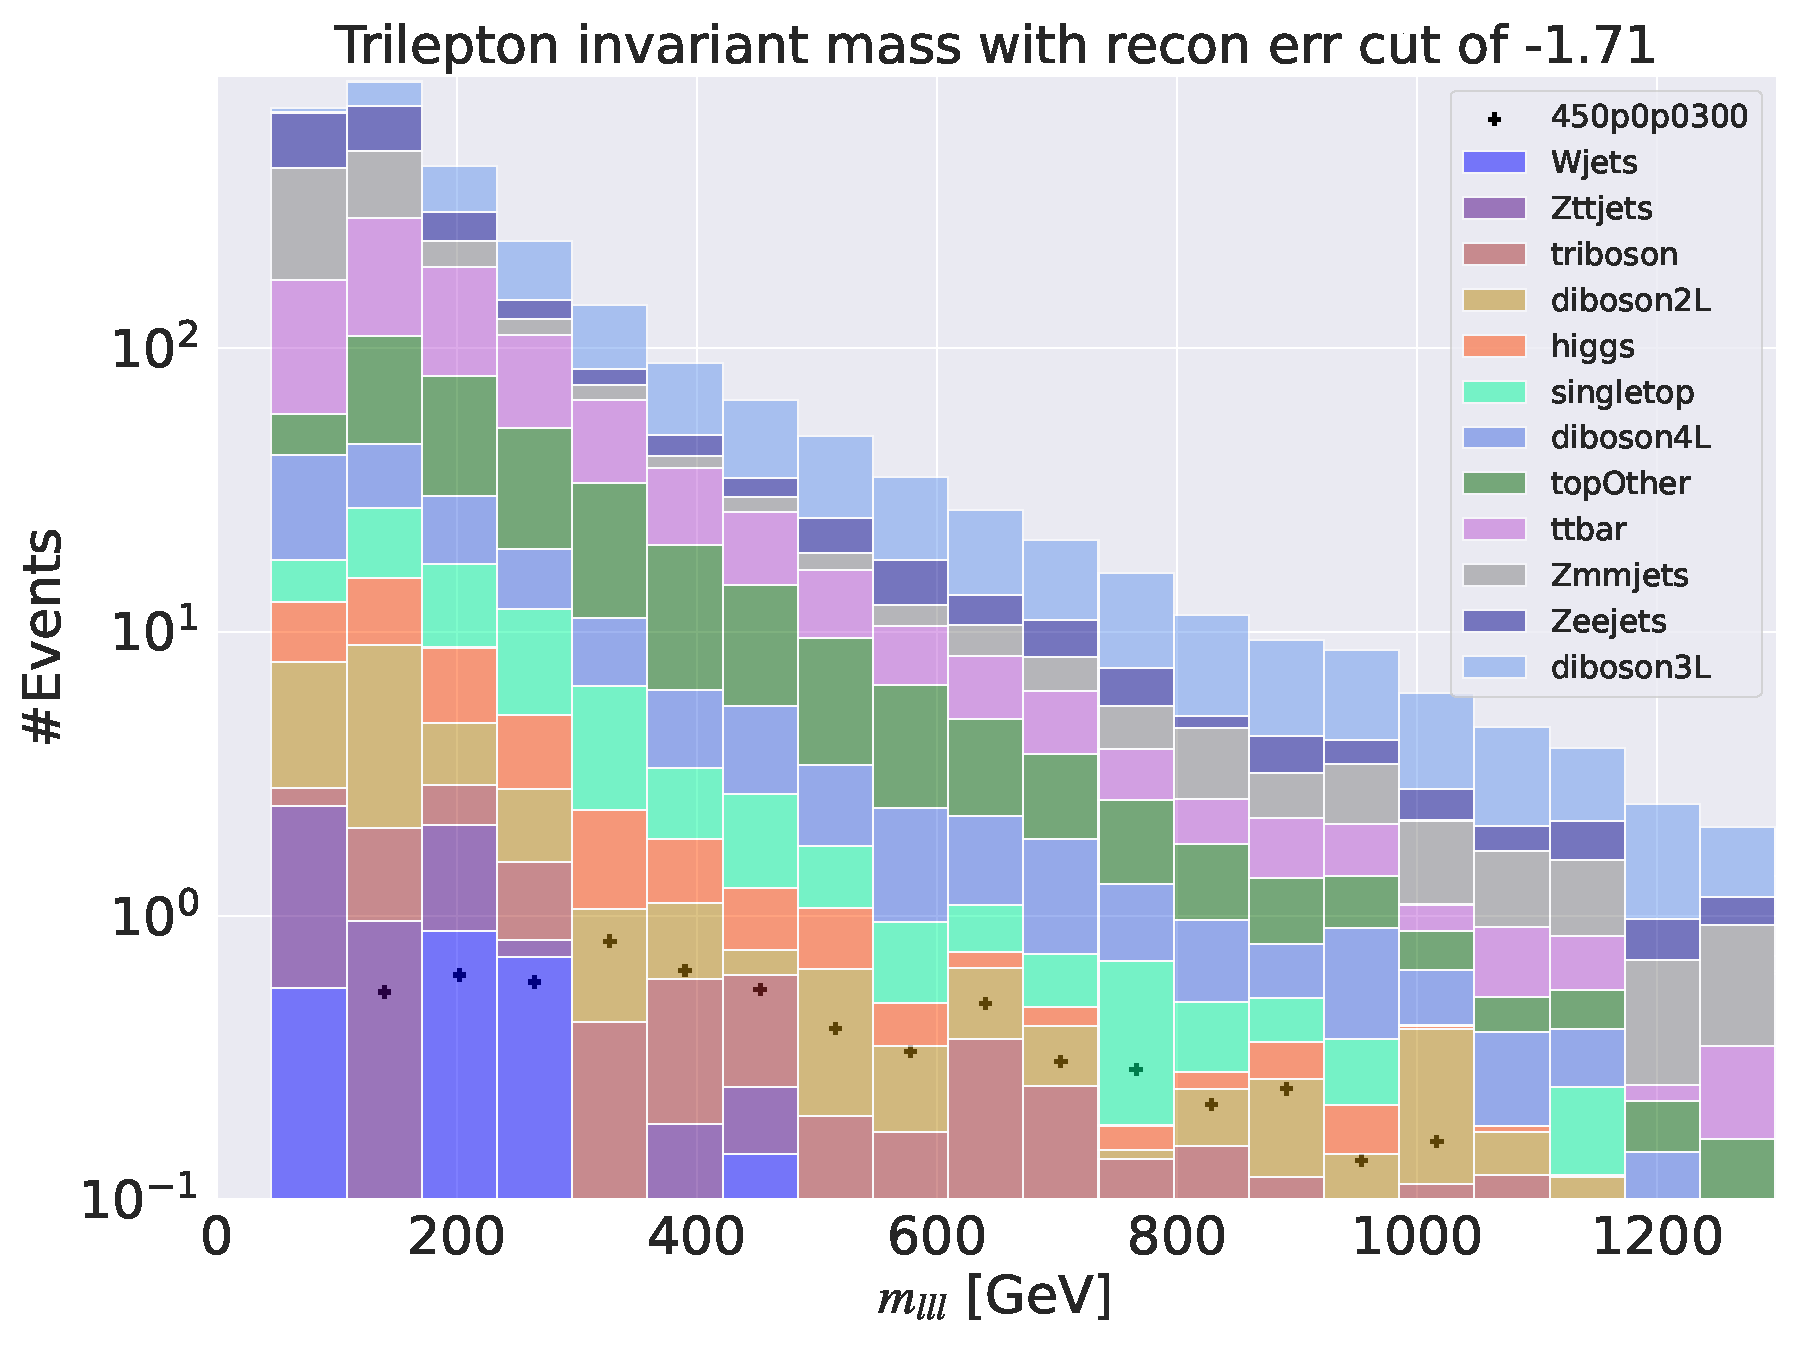
\includegraphics[width=\textwidth]{Figures/AE_testing/small/3lep/b_data_recon_big_rm3_feats_sig_450p0p0300_mlll_recon_errcut_-1.71.pdf}
        \caption{}
        \label{fig:AE_3lep_small_mlll_450}
    \end{subfigure}
    \hfill   
    \begin{subfigure}{.49\textwidth}
        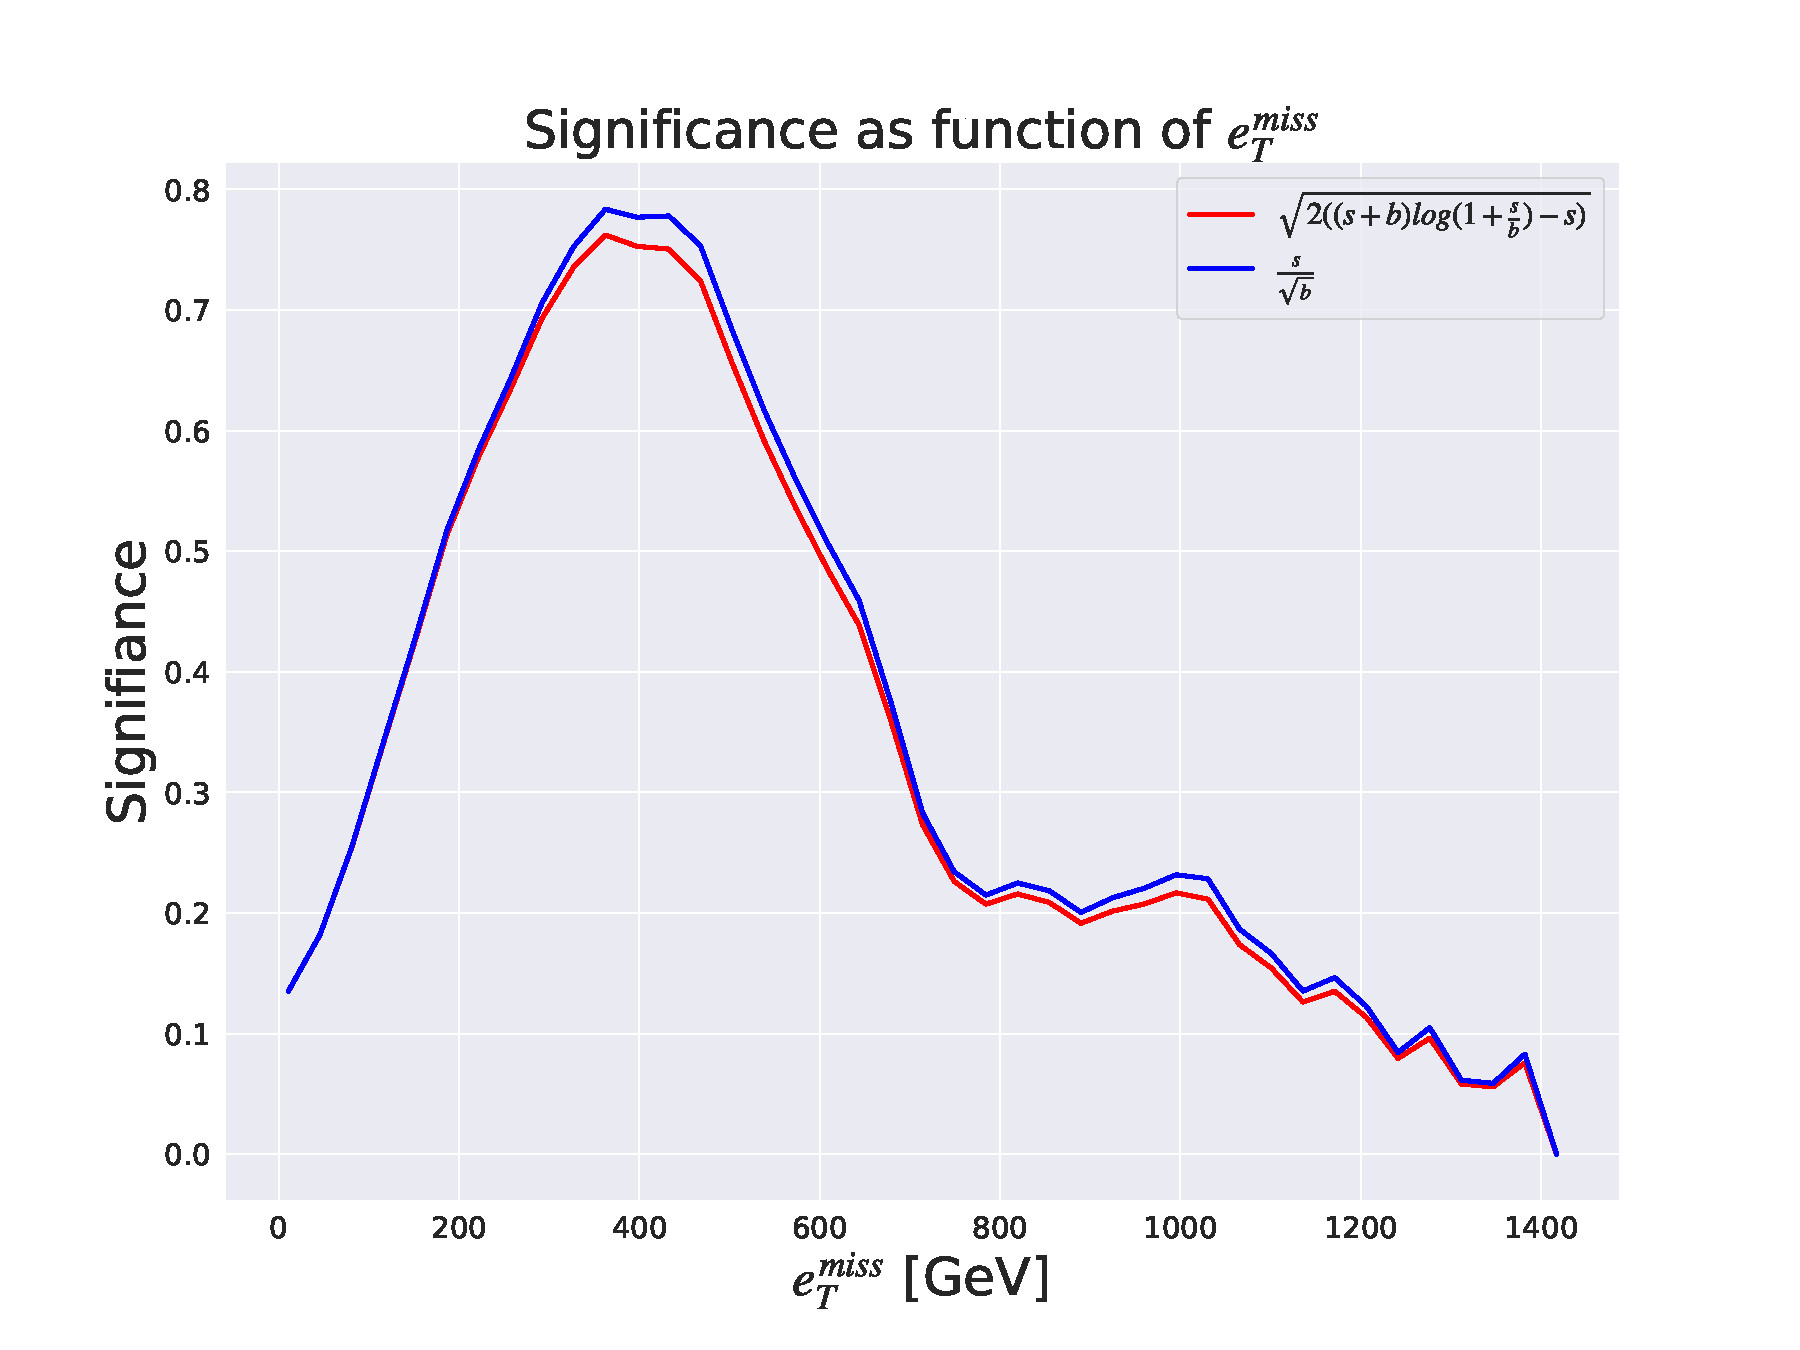
\includegraphics[width=\textwidth]{Figures/AE_testing/small/3lep/significance_etmiss_450p0p0300_-1.7067960296617328.pdf}
        \caption{}
        \label{fig:AE_3lep_small_signi_450}
    \end{subfigure}
    \hfill      
    \caption[3lep shallow network | $450p300$ | AE]{Reconstruction error, $e_T^{miss}$ signal region, $m_{lll}$ signal region and significance as function of 
    $e_T^{miss}$ for the shallow regular autoencoder using the SUSY $450p300$ model.}
    \label{fig:AE_3lep_small_rec_sig_signi_450}
\end{figure}








\begin{figure}[H]
    \centering
    \begin{subfigure}{.49\textwidth}
        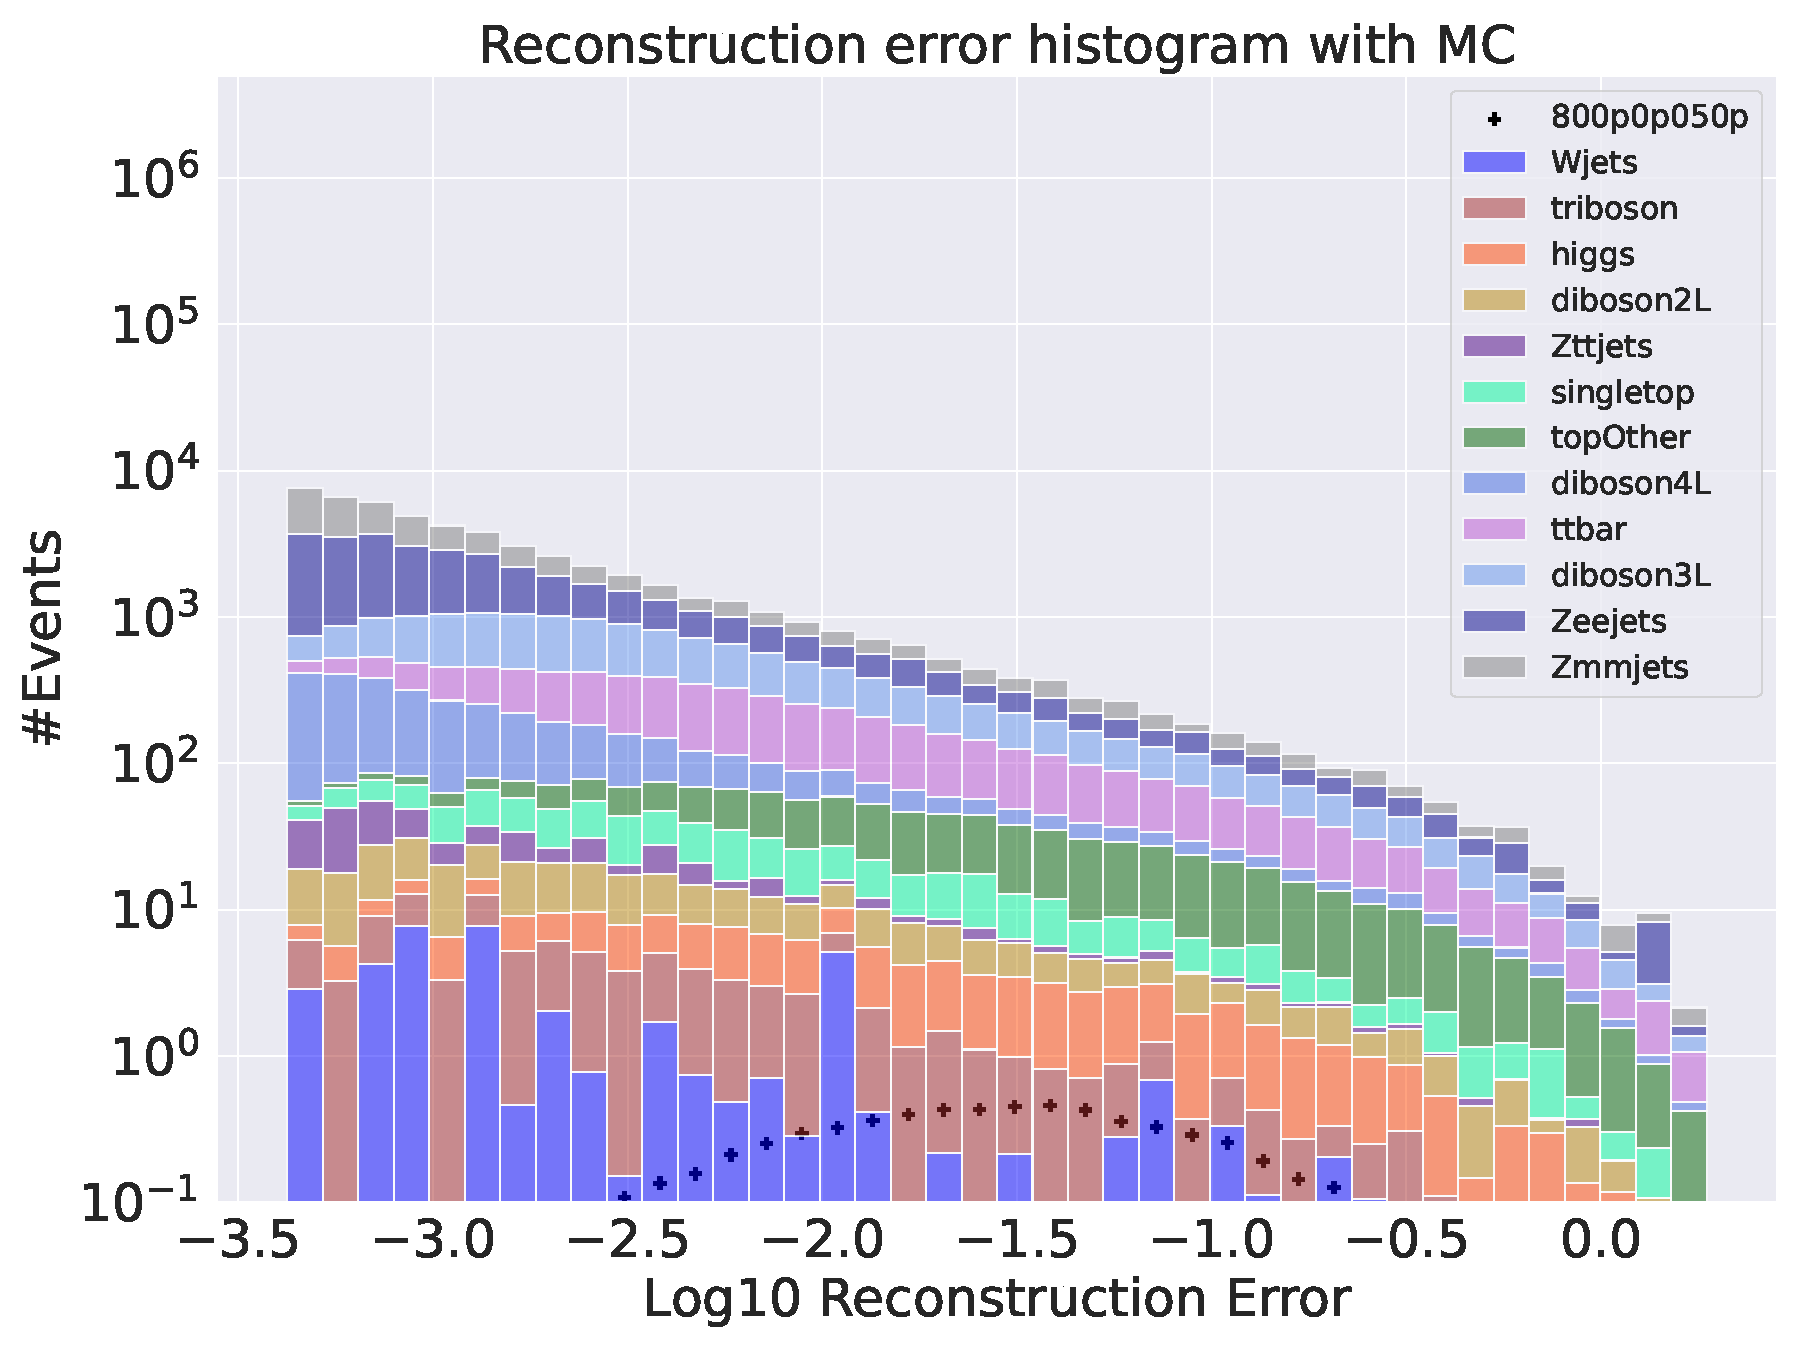
\includegraphics[width=\textwidth]{Figures/AE_testing/big/3lep/b_data_recon_big_rm3_feats_sig_800p0p050p.pdf}
        \caption{ }
        \label{fig:AE_3lep_big_800}
    \end{subfigure}
    \hfill
    \begin{subfigure}{.49\textwidth}
        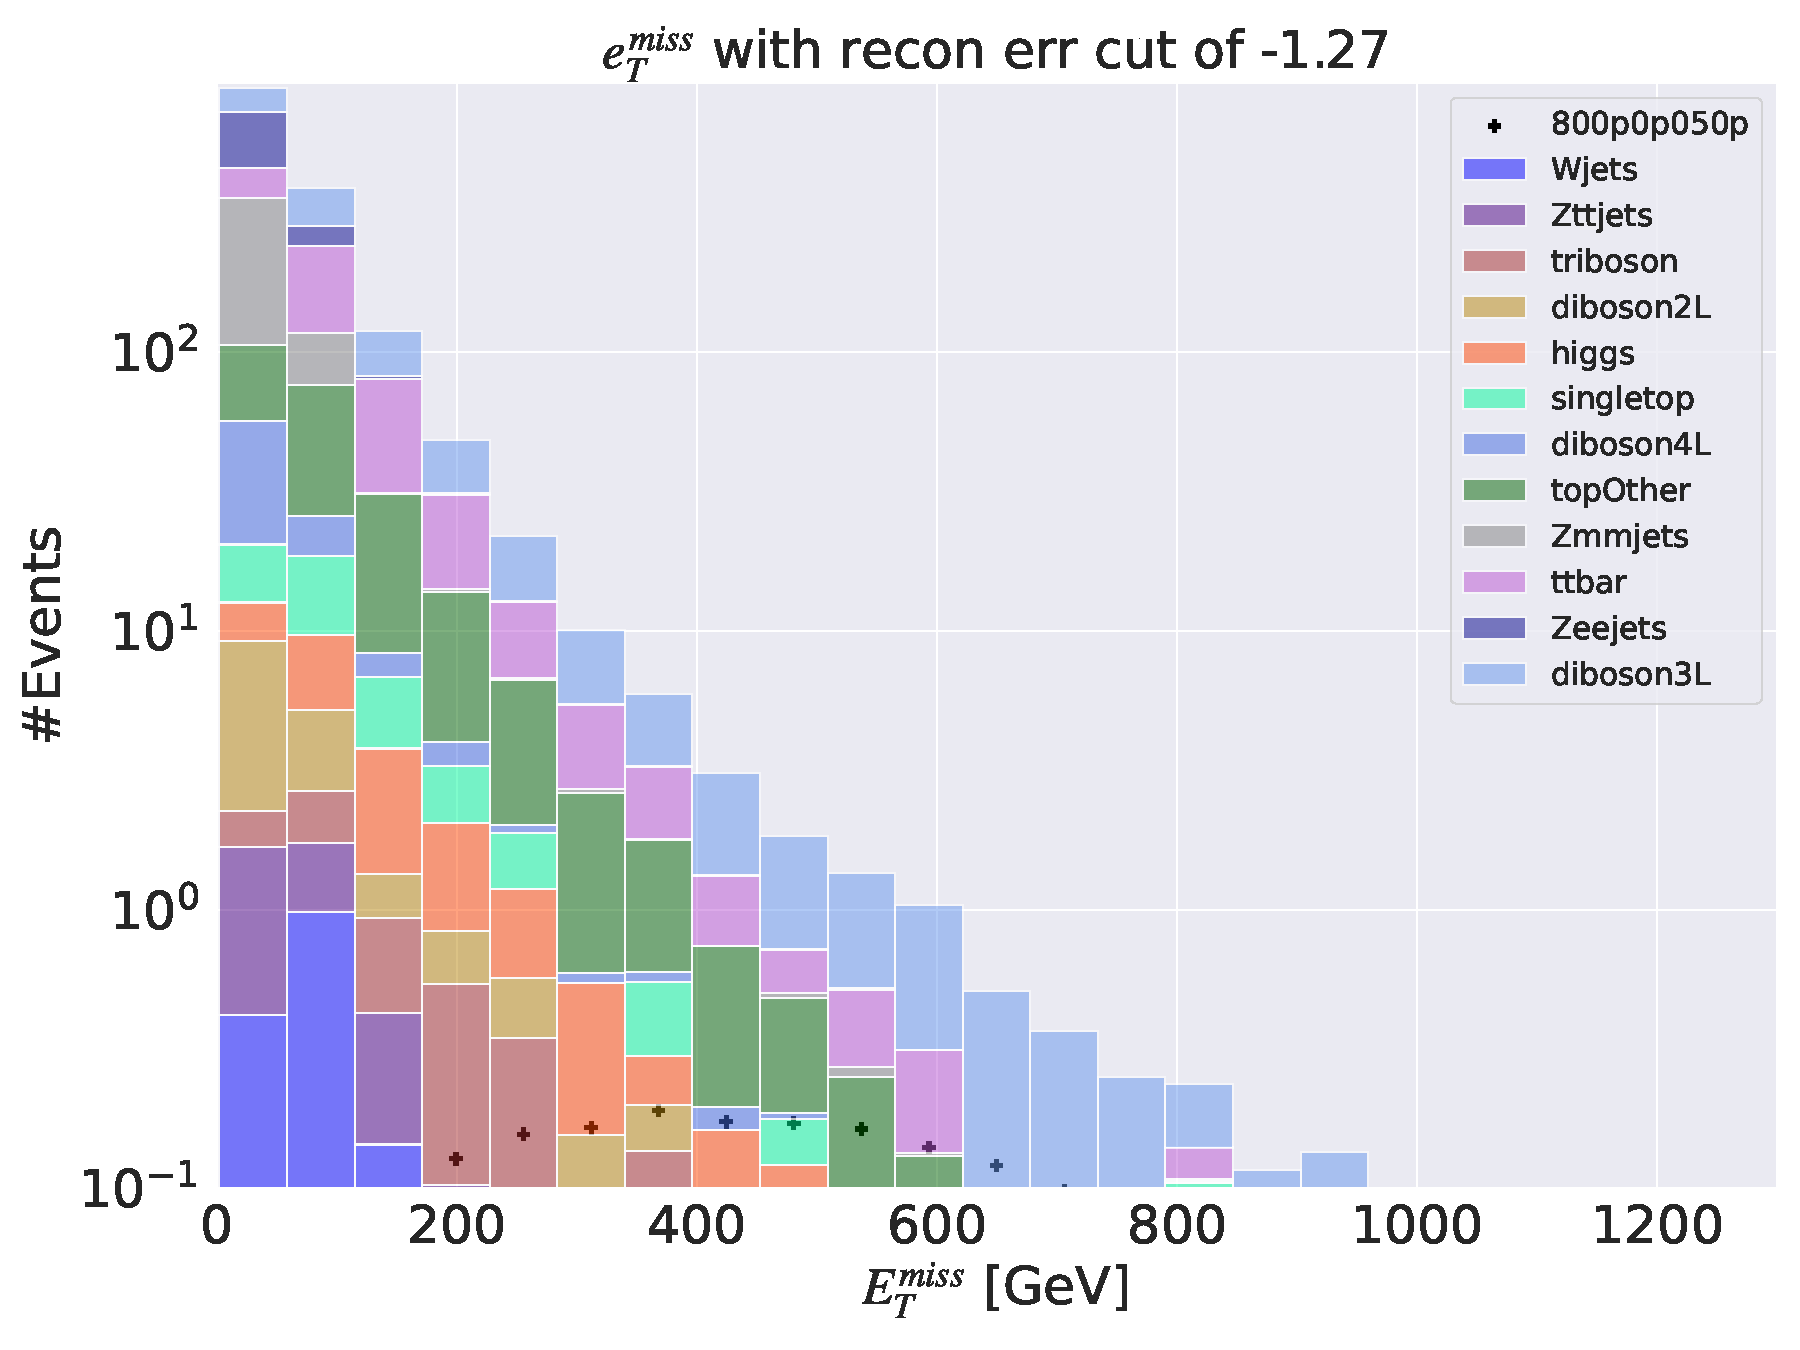
\includegraphics[width=\textwidth]{Figures/AE_testing/big/3lep/b_data_recon_big_rm3_feats_sig_800p0p050p_etmiss_recon_errcut_-1.27.pdf}
        \caption{}
        \label{fig:AE_3lep_big_etmiss_800}
    \end{subfigure}
    \hfill
    \begin{subfigure}{.49\textwidth}
        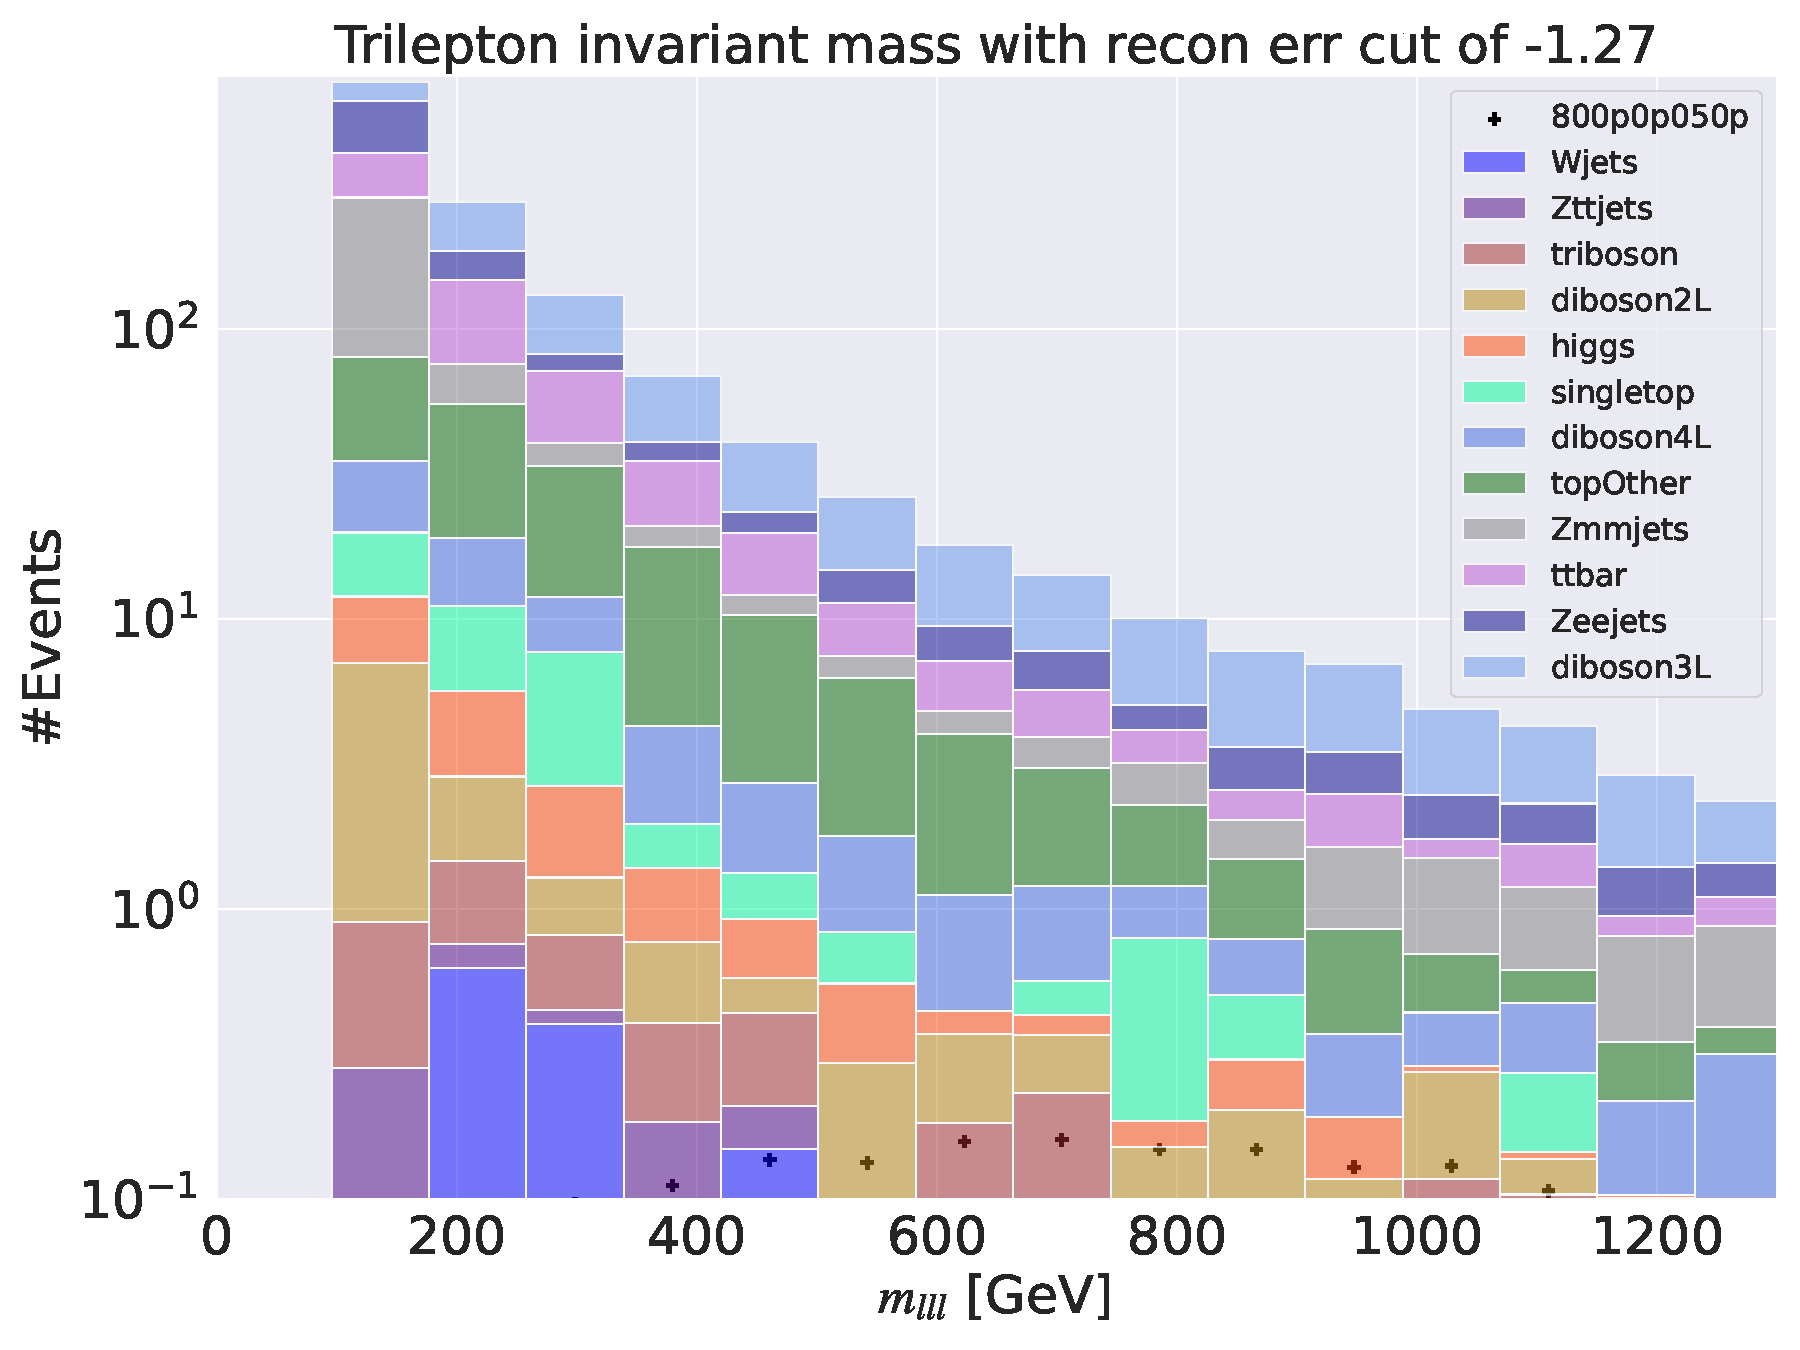
\includegraphics[width=\textwidth]{Figures/AE_testing/big/3lep/b_data_recon_big_rm3_feats_sig_800p0p050p_mlll_recon_errcut_-1.27.pdf}
        \caption{}
        \label{fig:AE_3lep_big_mlll_800}
    \end{subfigure}
    \hfill   
    \begin{subfigure}{.49\textwidth}
        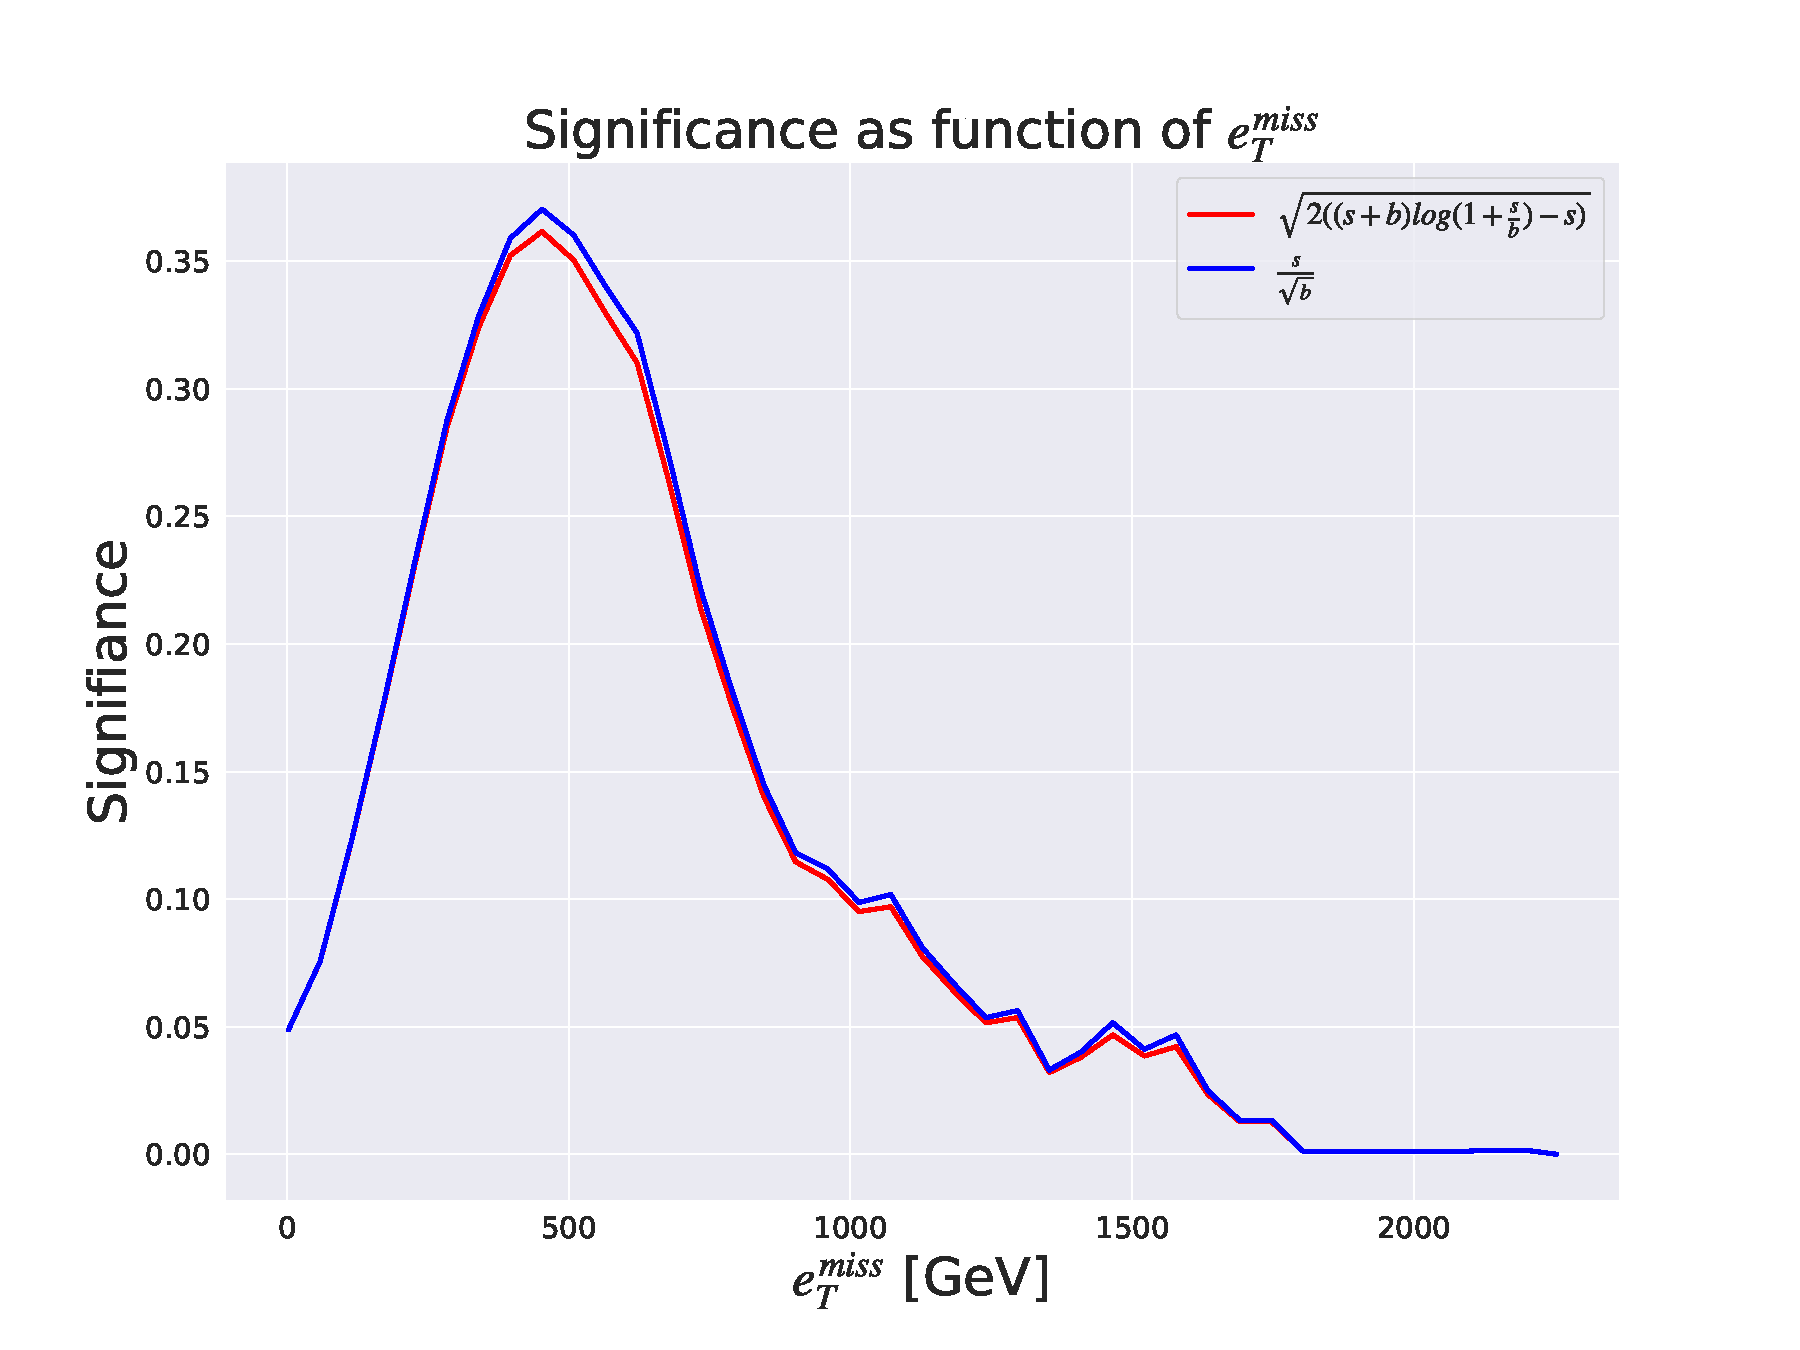
\includegraphics[width=\textwidth]{Figures/AE_testing/big/3lep/significance_etmiss_800p0p050p_-1.2726592563014343.pdf}
        \caption{}
        \label{fig:AE_3lep_big_signi_800}
    \end{subfigure}
    \hfill      
    \caption[3lep deep network | $800p50$ | AE]{Reconstruction error, $e_T^{miss}$ signal region, $m_{lll}$ signal region and significance as function of 
    $e_T^{miss}$ for the deep regular autoencoder using the SUSY $800p50$.}
    \label{fig:AE_3lep_big_rec_sig_signi_800}
\end{figure}

\begin{figure}[H]
    \centering
    \begin{subfigure}{.49\textwidth}
        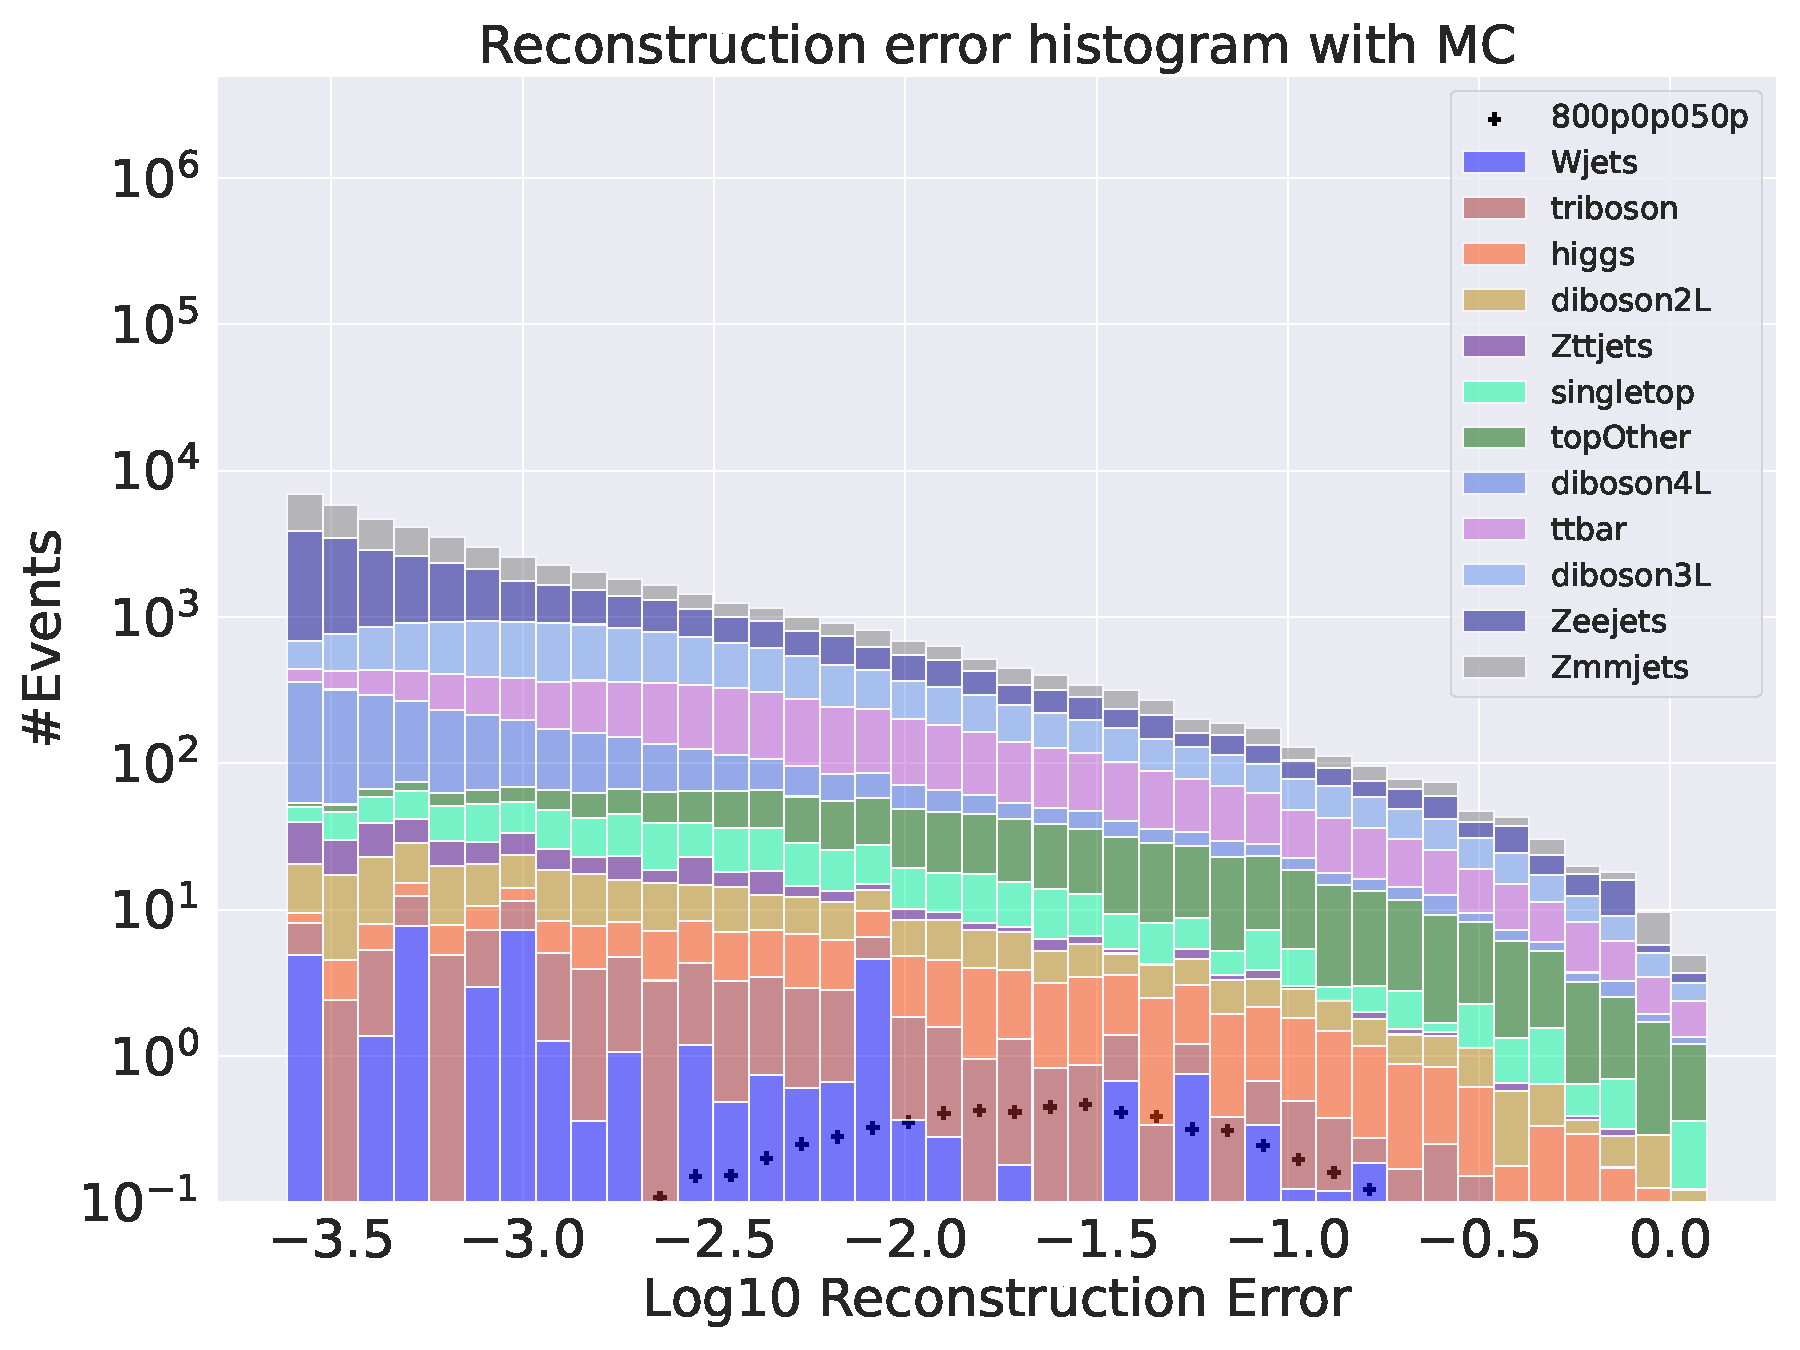
\includegraphics[width=\textwidth]{Figures/AE_testing/small/3lep/b_data_recon_big_rm3_feats_sig_800p0p050p.pdf}
        \caption{ }
        \label{fig:AE_3lep_small_800}
    \end{subfigure}
    \hfill
    \begin{subfigure}{.49\textwidth}
        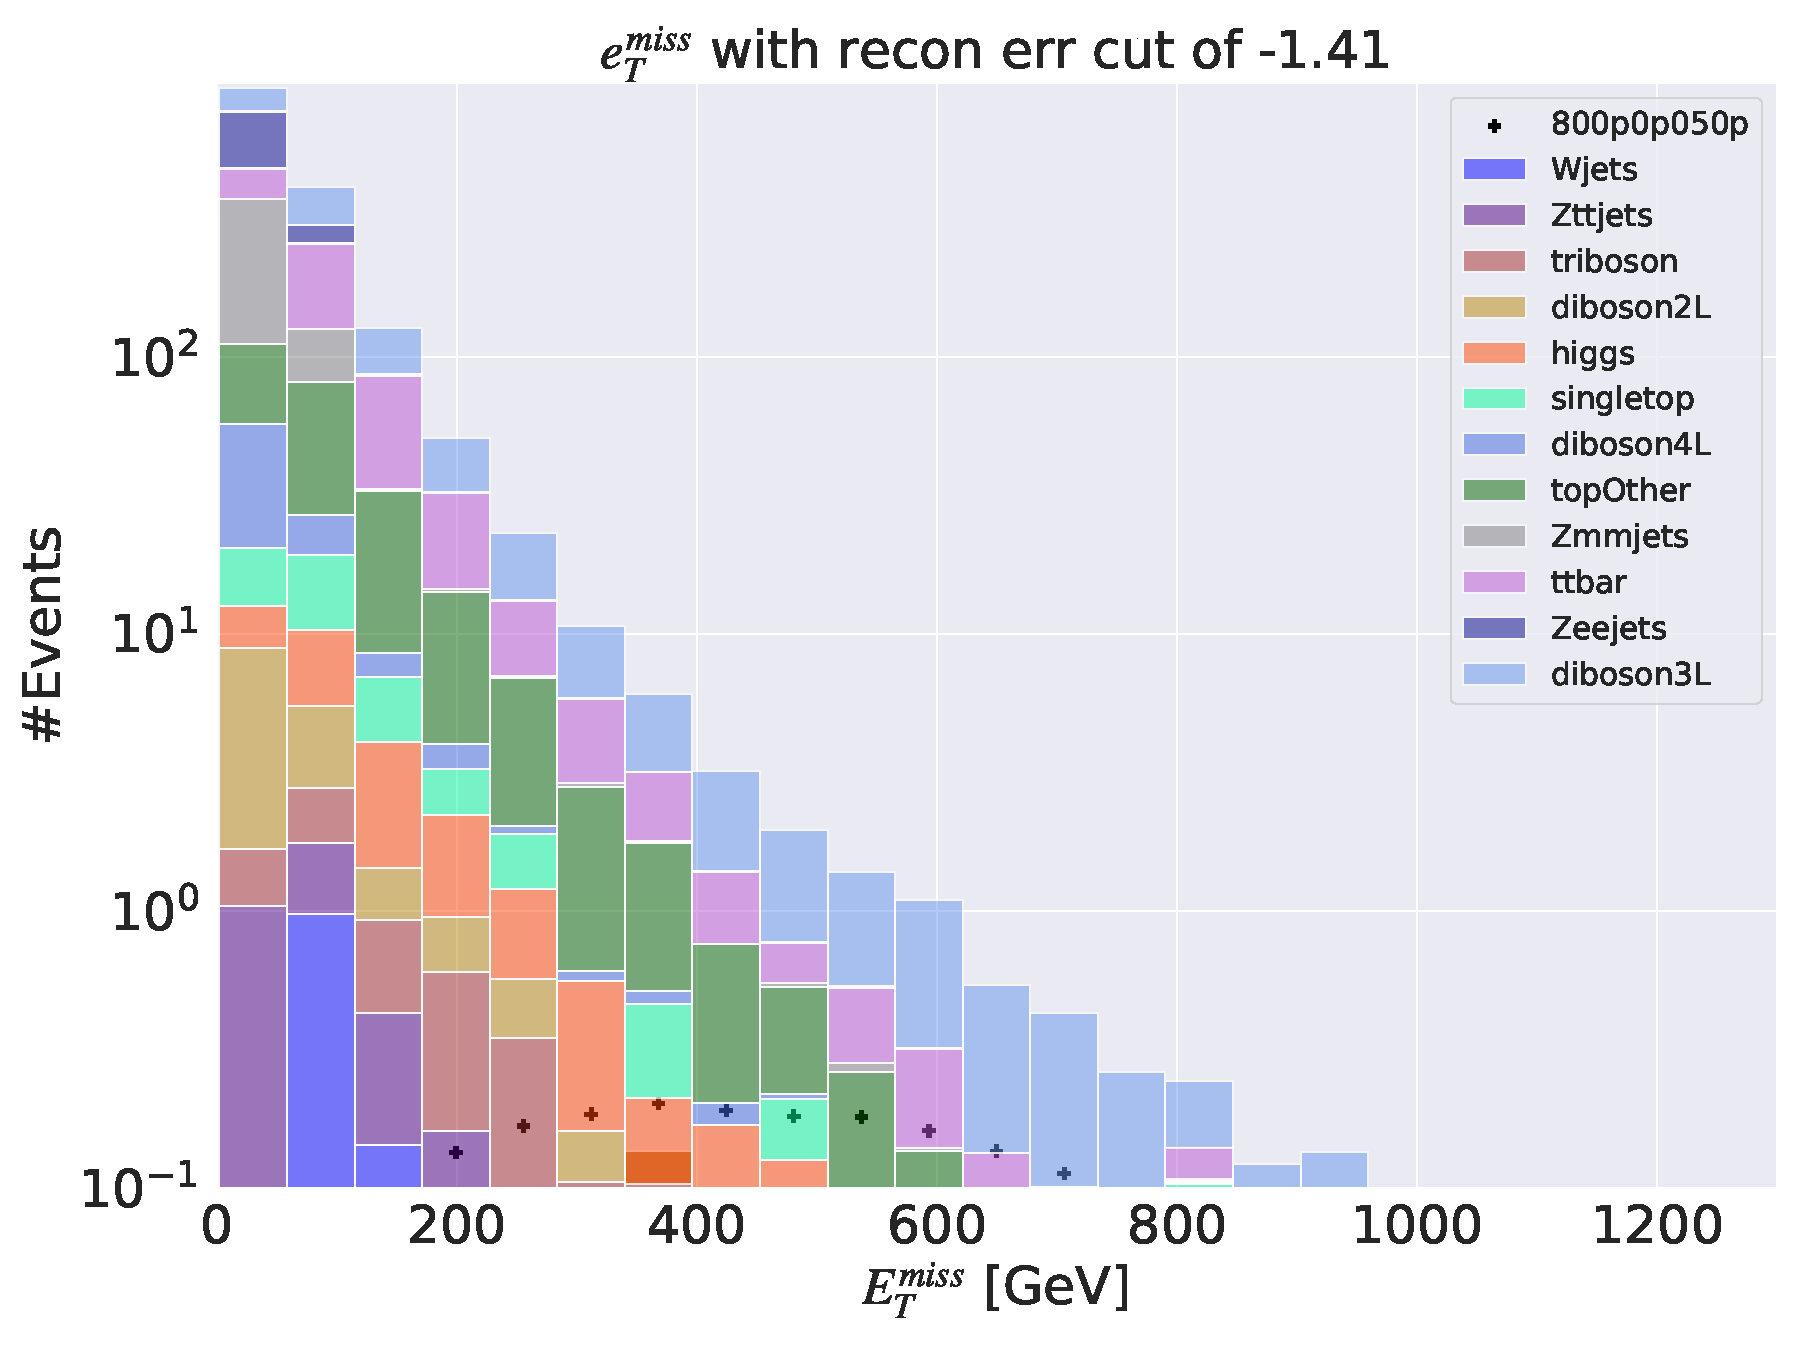
\includegraphics[width=\textwidth]{Figures/AE_testing/small/3lep/b_data_recon_big_rm3_feats_sig_800p0p050p_etmiss_recon_errcut_-1.41.pdf}
        \caption{}
        \label{fig:AE_3lep_small_etmiss_800}
    \end{subfigure}
    \hfill
    \begin{subfigure}{.49\textwidth}
        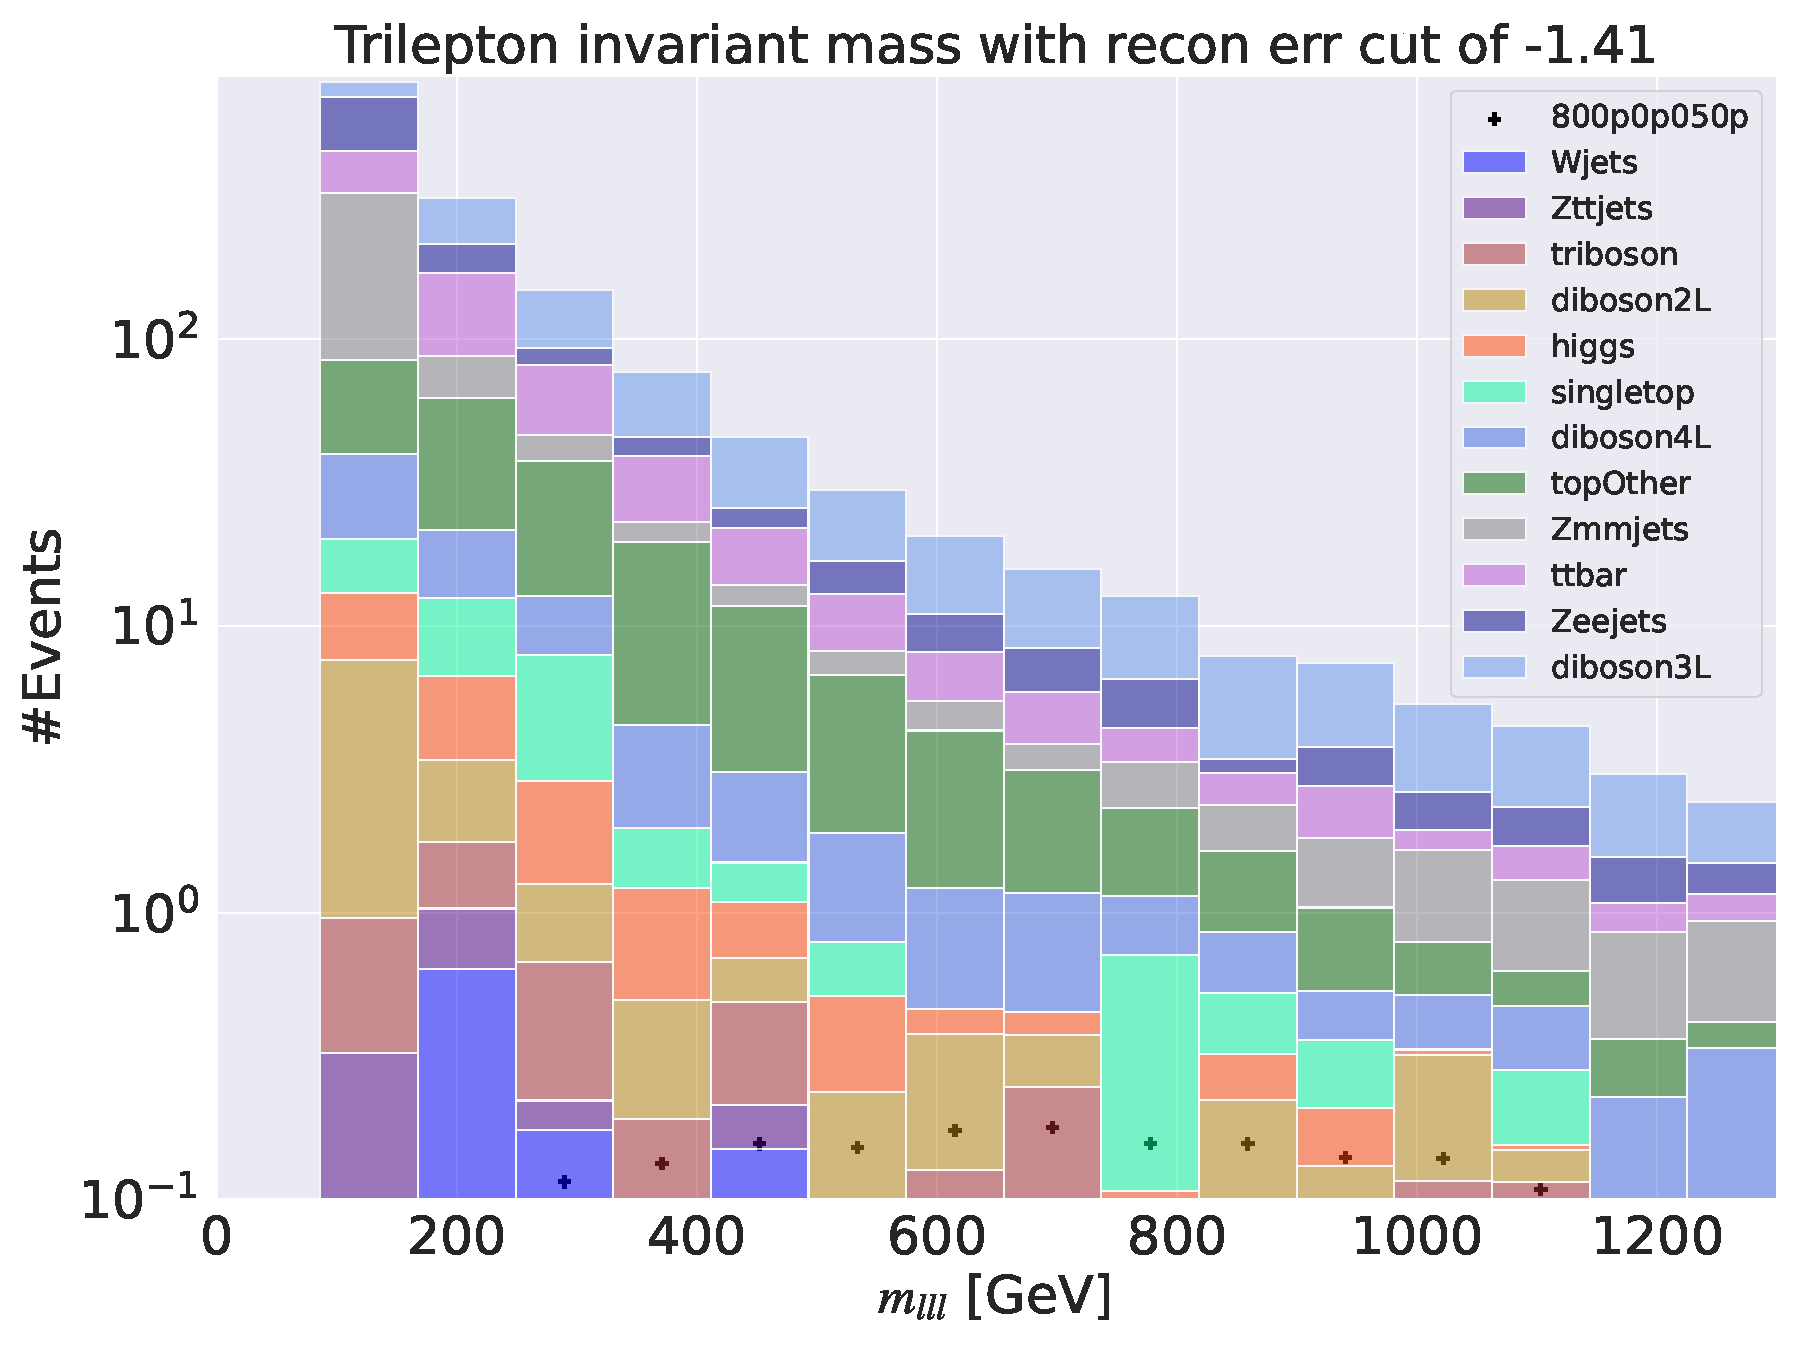
\includegraphics[width=\textwidth]{Figures/AE_testing/small/3lep/b_data_recon_big_rm3_feats_sig_800p0p050p_mlll_recon_errcut_-1.41.pdf}
        \caption{}
        \label{fig:AE_3lep_small_mlll_800}
    \end{subfigure}
    \hfill   
    \begin{subfigure}{.49\textwidth}
        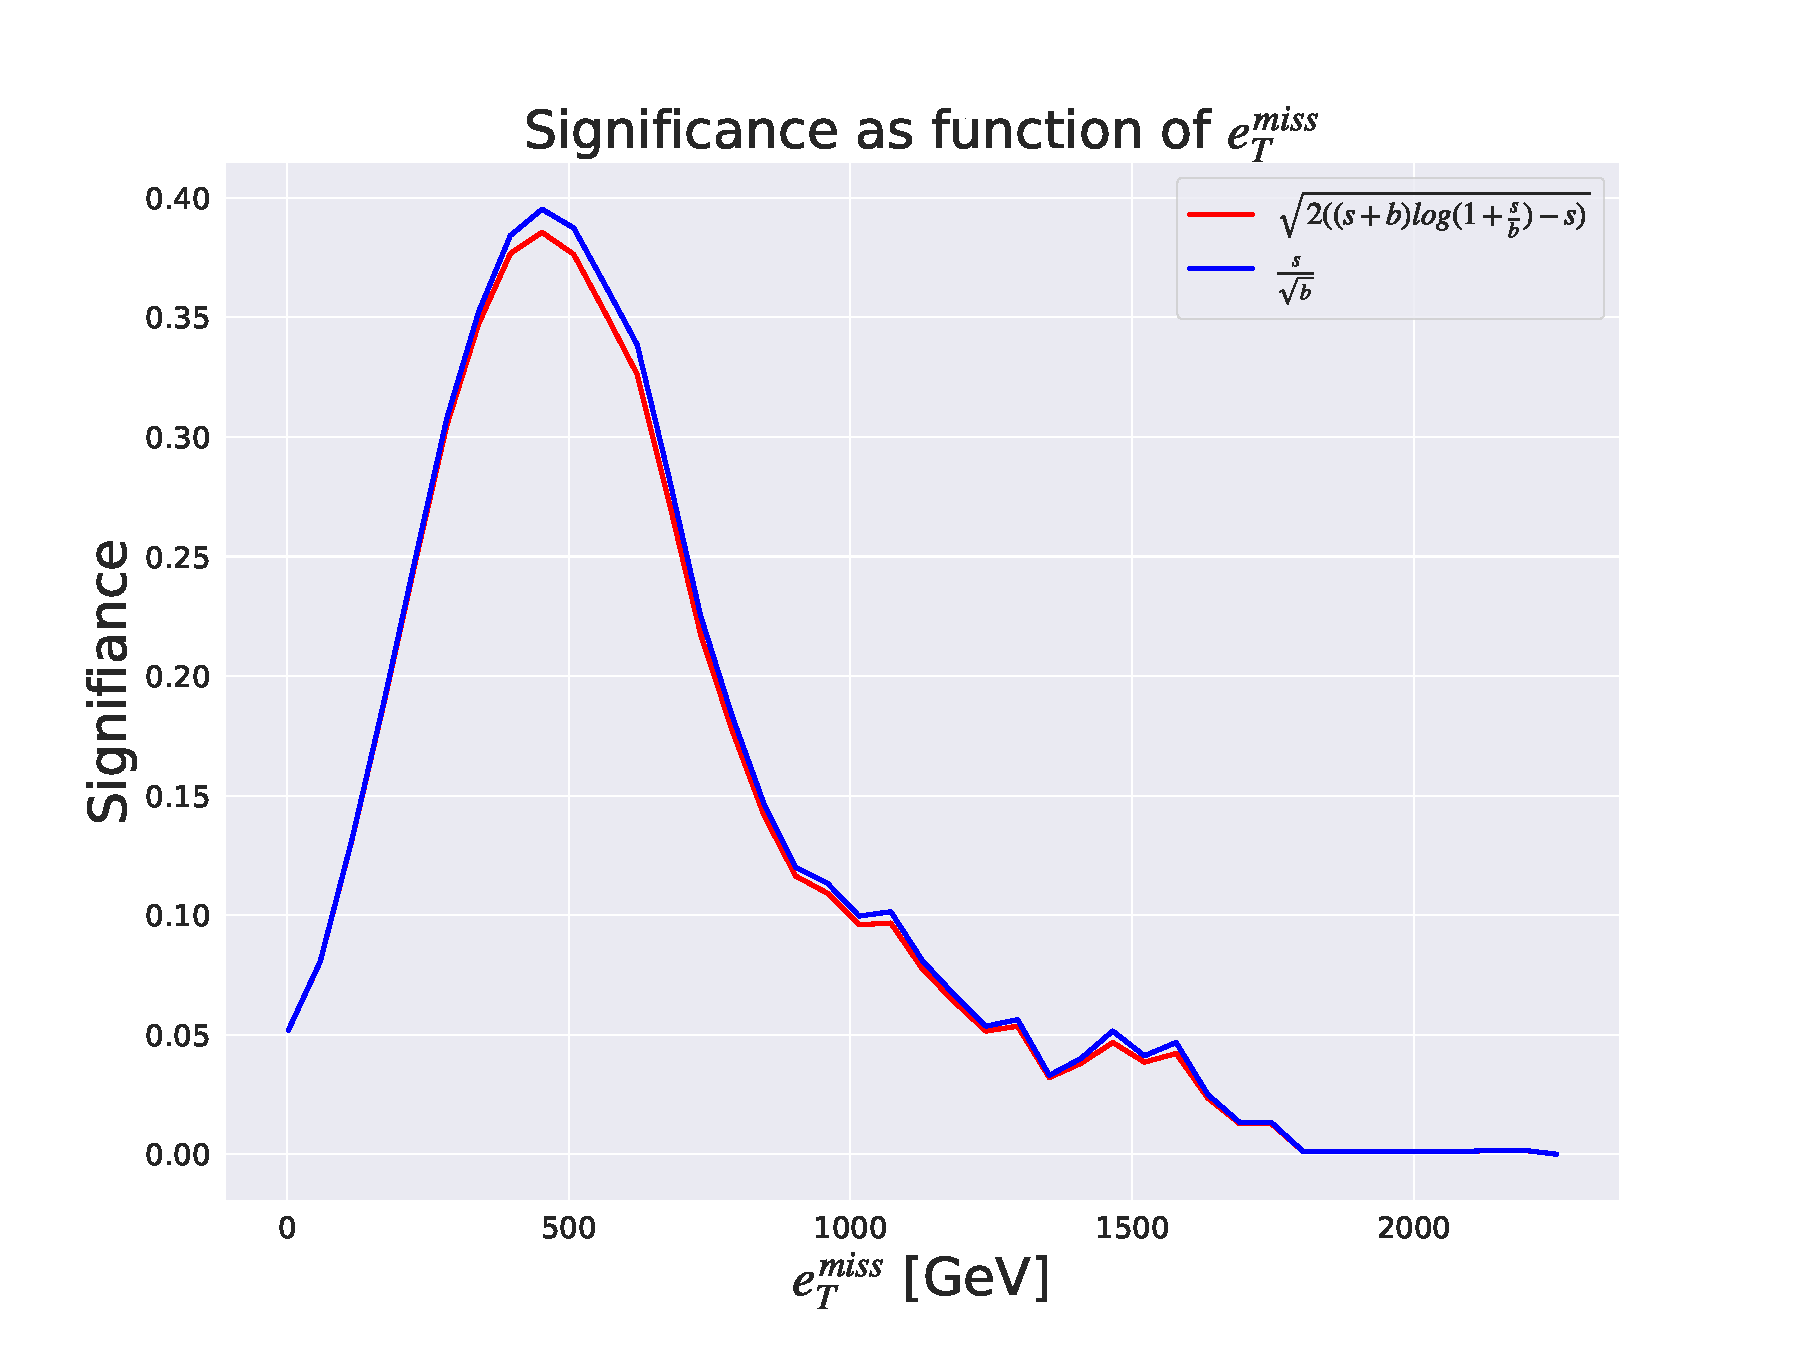
\includegraphics[width=\textwidth]{Figures/AE_testing/small/3lep/significance_etmiss_800p0p050p_-1.4089386402528896.pdf}
        \caption{}
        \label{fig:AE_3lep_small_signi_800}
    \end{subfigure}
    \hfill      
    \caption[3lep shallow network | $800p50$ | AE]{Reconstruction error, $e_T^{miss}$ signal region, $m_{lll}$ signal region and significance as function of 
    $e_T^{miss}$ for the shallow regular autoencoder using the SUSY $800p50$.}
    \label{fig:AE_3lep_small_rec_sig_signi_800}
\end{figure}

In figures \ref{fig:AE_3lep_big_rec_sig_signi_450}, \ref{fig:AE_3lep_small_rec_sig_signi_450}, 
\ref{fig:AE_3lep_big_rec_sig_signi_800} and \ref{fig:AE_3lep_small_rec_sig_signi_800} we have four 
subplots containing the total reconstruction error distributions, the $e_T^{miss}$ signal region, 
the $m_{lll}$ signal region and the significance as function of $e_T^{miss}$ curve respectively 
for the shallow and deep regular autoencoder. From figures \ref{fig:AE_3lep_big_450}, 
\ref{fig:AE_3lep_small_450}, \ref{fig:AE_3lep_big_800}, \ref{fig:AE_3lep_small_800} it is clear 
here that the autoencoder manages to somewhat separate the peaks of the signal and background 
distributions. Still, the distributions themselves are not separated. The 
SUSY $800p50$ signals has the best separation of peaks, which is expected considering its 
rather extreme tail in the $e_T^{miss}$ distribution of the signal. It is also interesting to 
observe the slope trend in the SM MC reconstruciton error distribution. The steepness of the 
slope seems to be somewhat similar for both the shallow and deep regular autoencoder, indicating 
at least that the difference in these two models does not differ much when it comes to performance. 
The bulk of the events are below $10^{-2}$ reconstruction error, indicating that the autoencoder 
has learned a lot of the internal RMM structures for the 3 lepton + $e_T^{miss}$ final state MC. \par
In figures \ref{fig:AE_3lep_big_etmiss_450}, \ref{fig:AE_3lep_small_etmiss_450}, 
\ref{fig:AE_3lep_big_etmiss_800} and  \ref{fig:AE_3lep_small_etmiss_800} we have a signal region 
created for each of the SUSY models from both the shallow and deep regular autoencoder. The cuts 
were created using the median and then iteratively increasing the error requirement, as 
explained in section \ref{sec:strategy}. Only one of the three cuts done are shown here, the 
rest can be found in the appendix. The histograms in figures \ref{fig:AE_3lep_big_etmiss_450}, 
\ref{fig:AE_3lep_small_etmiss_450}, \ref{fig:AE_3lep_big_etmiss_800} and  
\ref{fig:AE_3lep_small_etmiss_800} displays the $e_T^{miss}$ distribution in the signal region 
for the SM MC and the SUSY signals. They represent the signal region with the most relaxed cut, 
in other words, the least strict and thus the signal region with the most amount of total events, 
both SM MC and signal. This is to illustrate the difficulty of this method since we only have the 
reconstruction error to go on. Thus, too strict a cut will most likely eliminate all possible 
signal events in the signal region, whereas too loose a cut and the SM MC background will dominate completely.
In figures \ref{fig:AE_3lep_big_mlll_450}, \ref{fig:AE_3lep_small_mlll_450}, \ref{fig:AE_3lep_big_mlll_800} and  
\ref{fig:AE_3lep_small_mlll_800} we have the  $m_{lll}$ distributions in the signal 
regions from both the shallow and deep regular 
autoencoder for both SUSY signals. As with the $e_T^{miss}$ distributions, the $m_{lll}$ distributions 
with the least strict cut in the signal region 
are shown here, with the rest shown in the appendix. From these figures it is not easy to see any resonances 
in the distributions. There is also little separation between signal and background distributions in 
the $m_{lll}$ feature, allthough there is some for the SUSY $800p50$ model. It is also 
shown that the difference between the shallow and deep neural network architecture has little to no effect 
here or in the $e_T^{miss}$ distributions in terms of separation.  \par 
In figures \ref{fig:AE_3lep_big_signi_450}, \ref{fig:AE_3lep_small_signi_450}, \ref{fig:AE_3lep_big_signi_800} and  
\ref{fig:AE_3lep_small_signi_800} we have the significance as a function of the $e_T^{miss}$. It displays that 
a further cut on the $e_T^{miss}$ will get an even better significance, the best case provided from the SUSY $450p300$
signal with the deep autoencoder, using a cut on the $e_T^{miss}$ around 400 GeV. 


\subsubsection*{Variational autoencoder output}
In the Variational autoencoder case, we have the same distributions as above. Below we have the full reconstruction 
error distributions for both signals from the shallow and deep variational autoencoder. 


\begin{figure}[H]
    \centering
    \begin{subfigure}{.49\textwidth}
        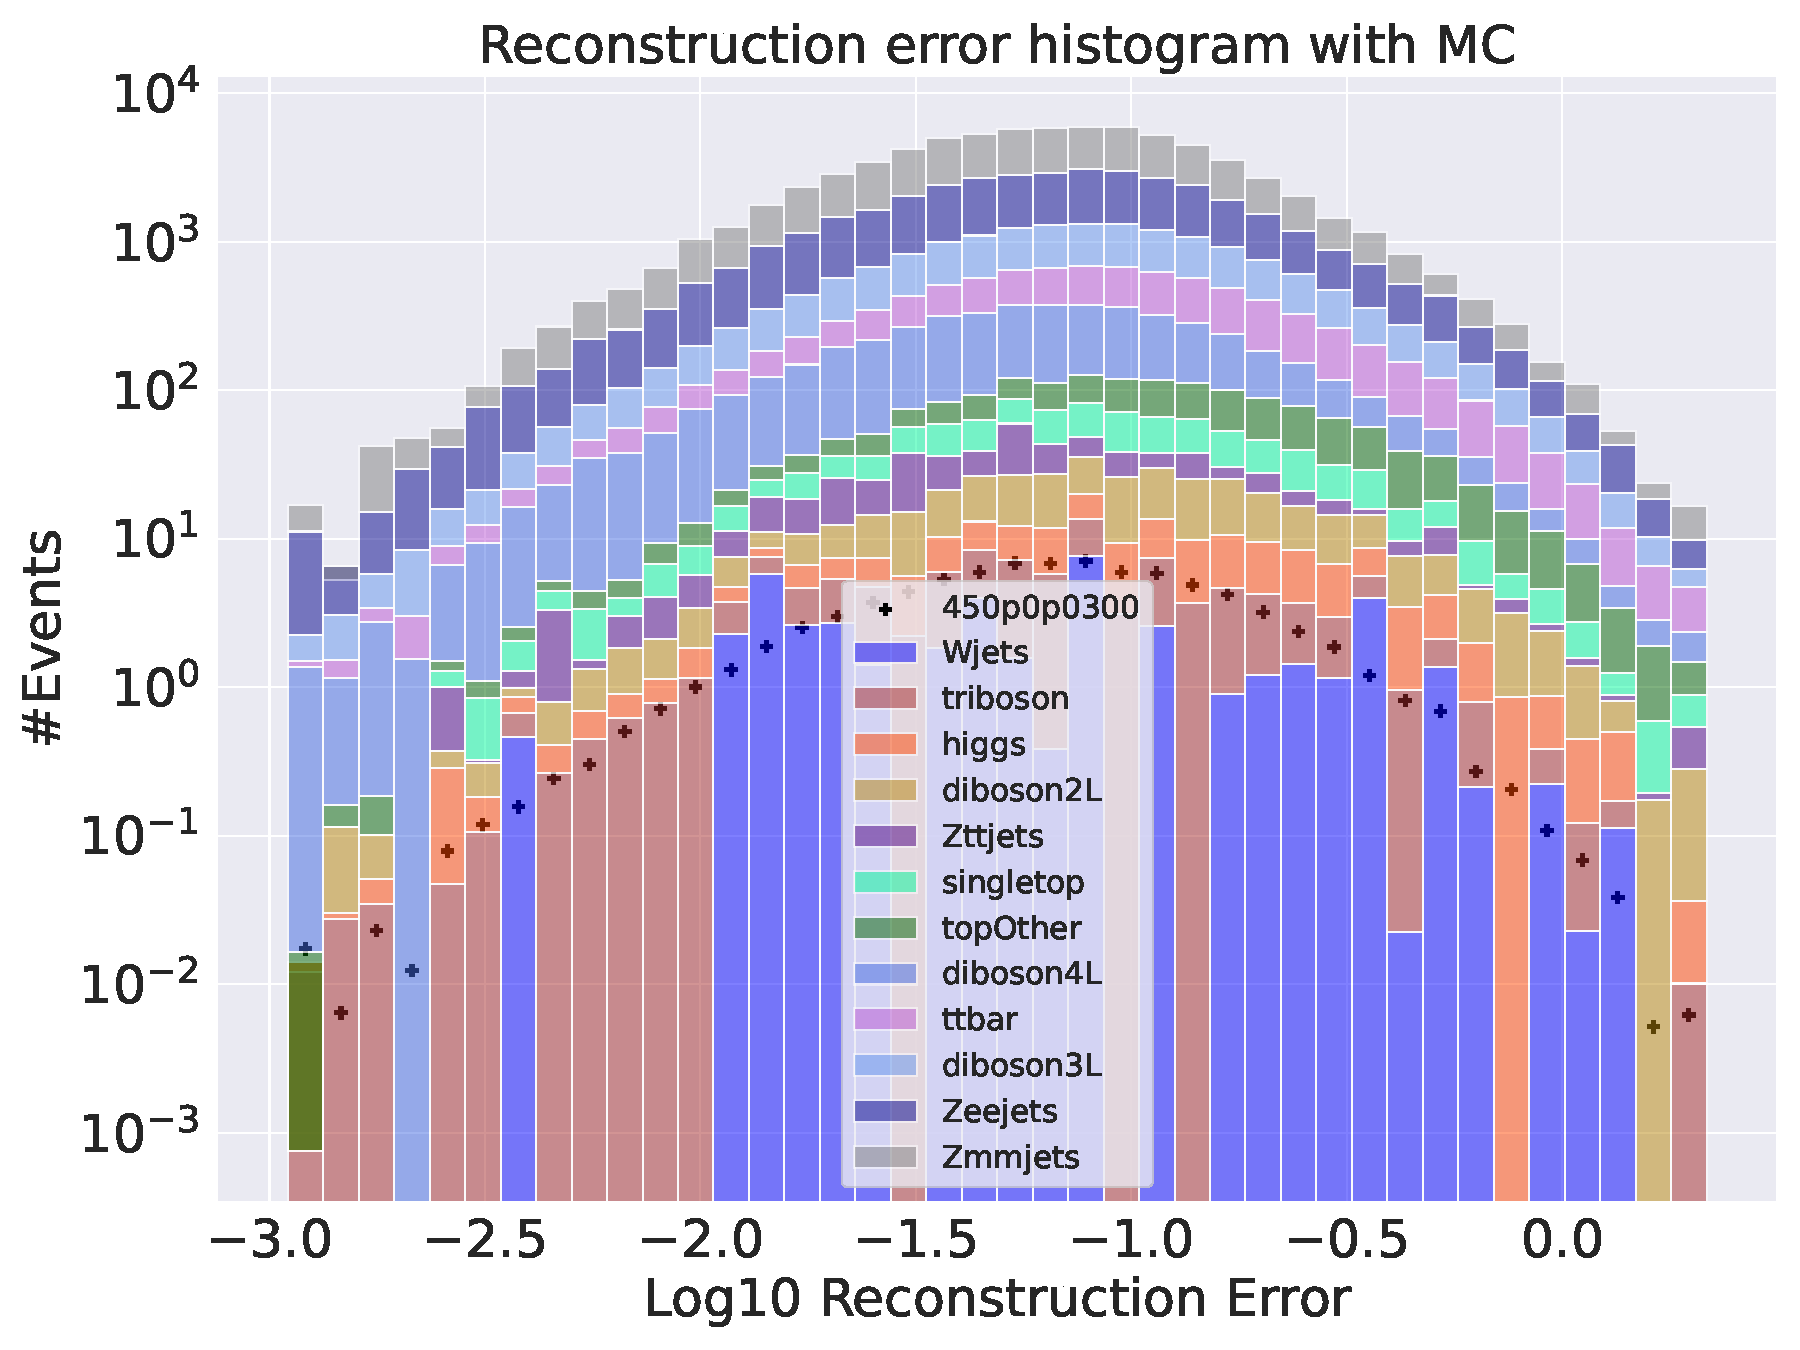
\includegraphics[width=\textwidth]{Figures/VAE_testing/big/3lep/b_data_recon_big_rm3_feats_sig_450p0p0300.pdf}
        \caption{ }
        \label{fig:VAE_3lep_big_450}
    \end{subfigure}
    \hfill
    \begin{subfigure}{.49\textwidth}
        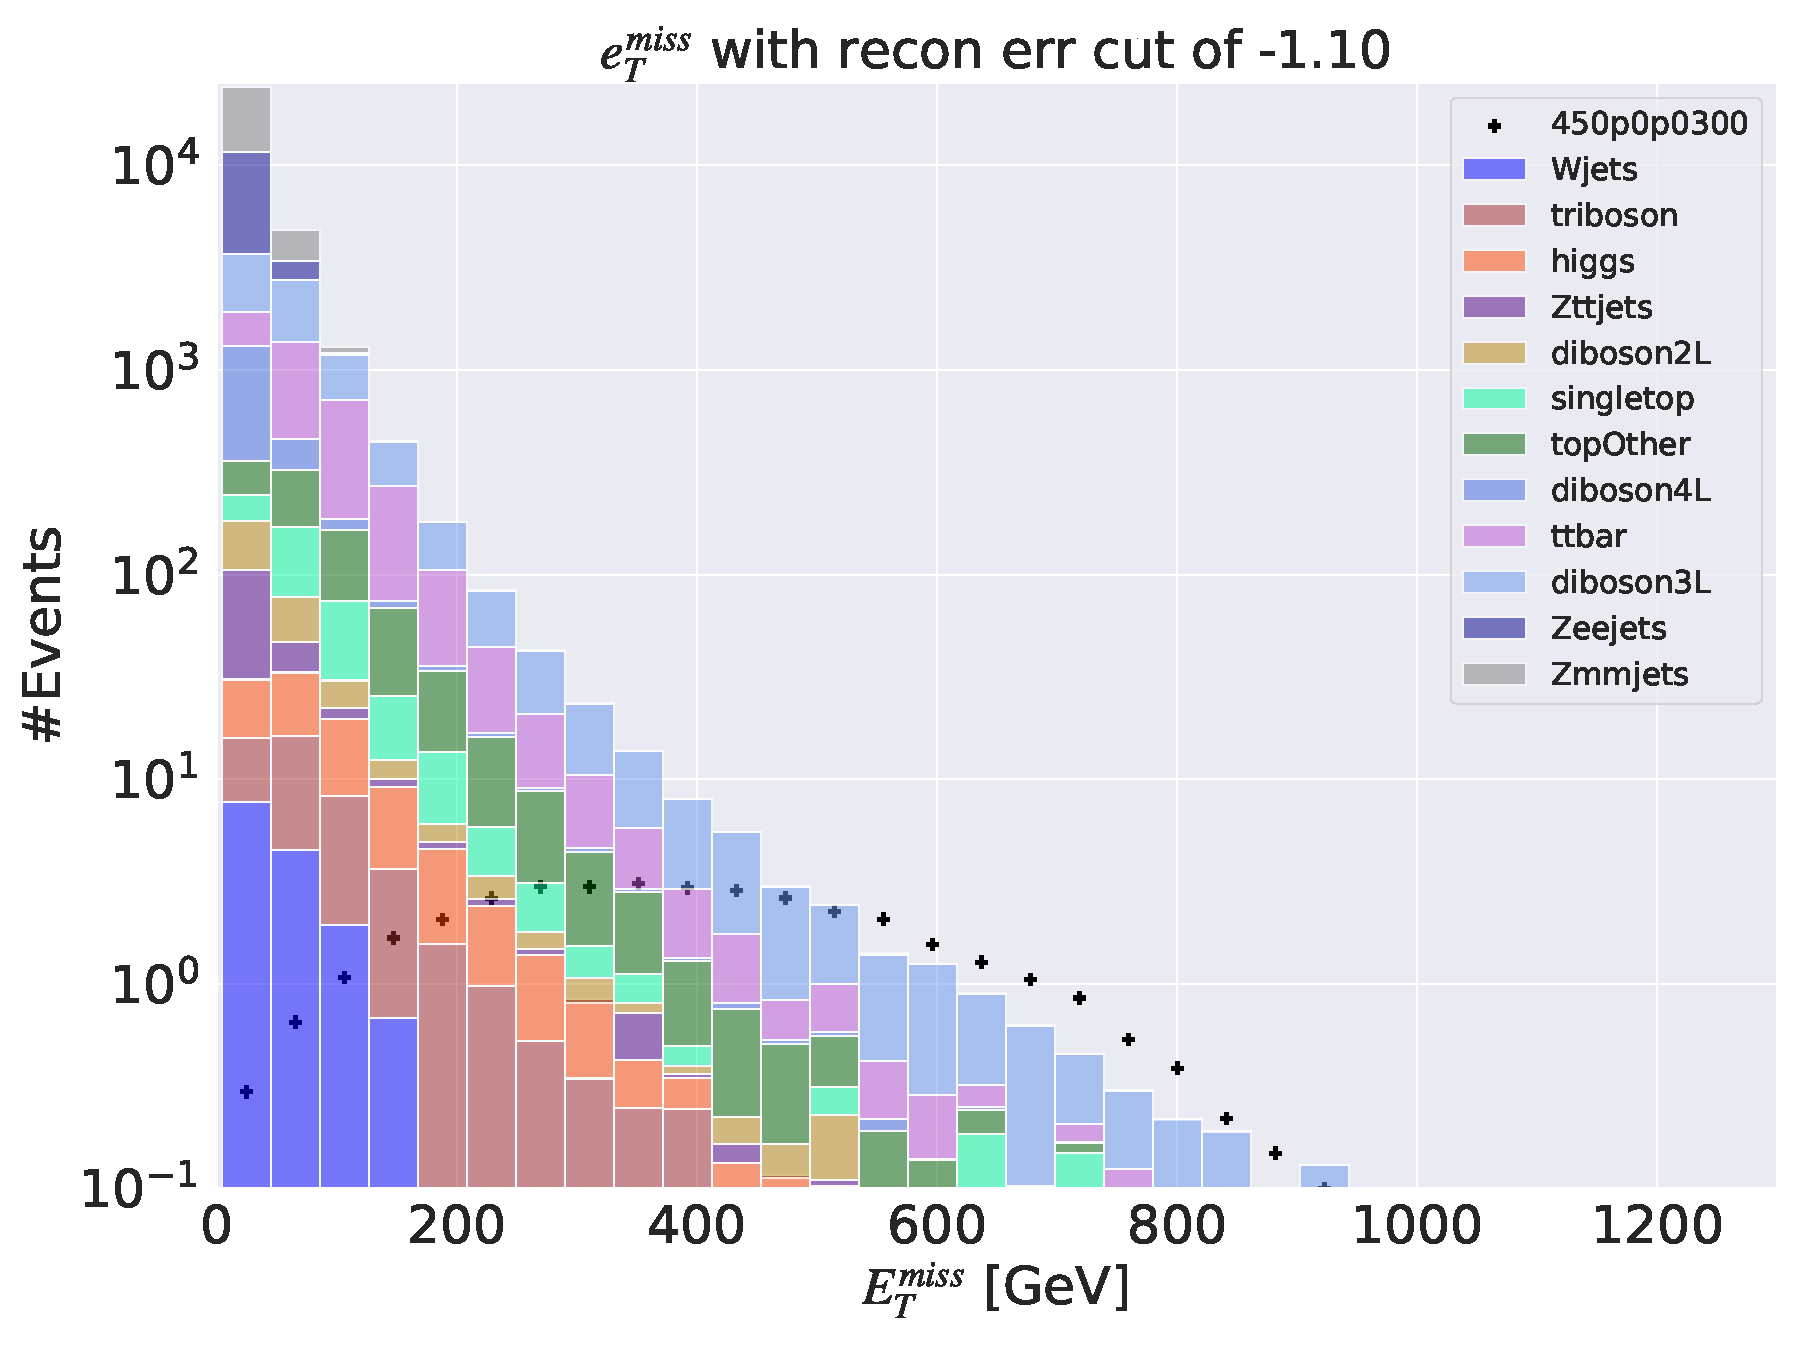
\includegraphics[width=\textwidth]{Figures/VAE_testing/big/3lep/b_data_recon_big_rm3_feats_sig_450p0p0300_etmiss_recon_errcut_-1.10.pdf}
        \caption{}
        \label{fig:VAE_3lep_big_etmiss_450}
    \end{subfigure}
    \hfill
    \begin{subfigure}{.49\textwidth}
        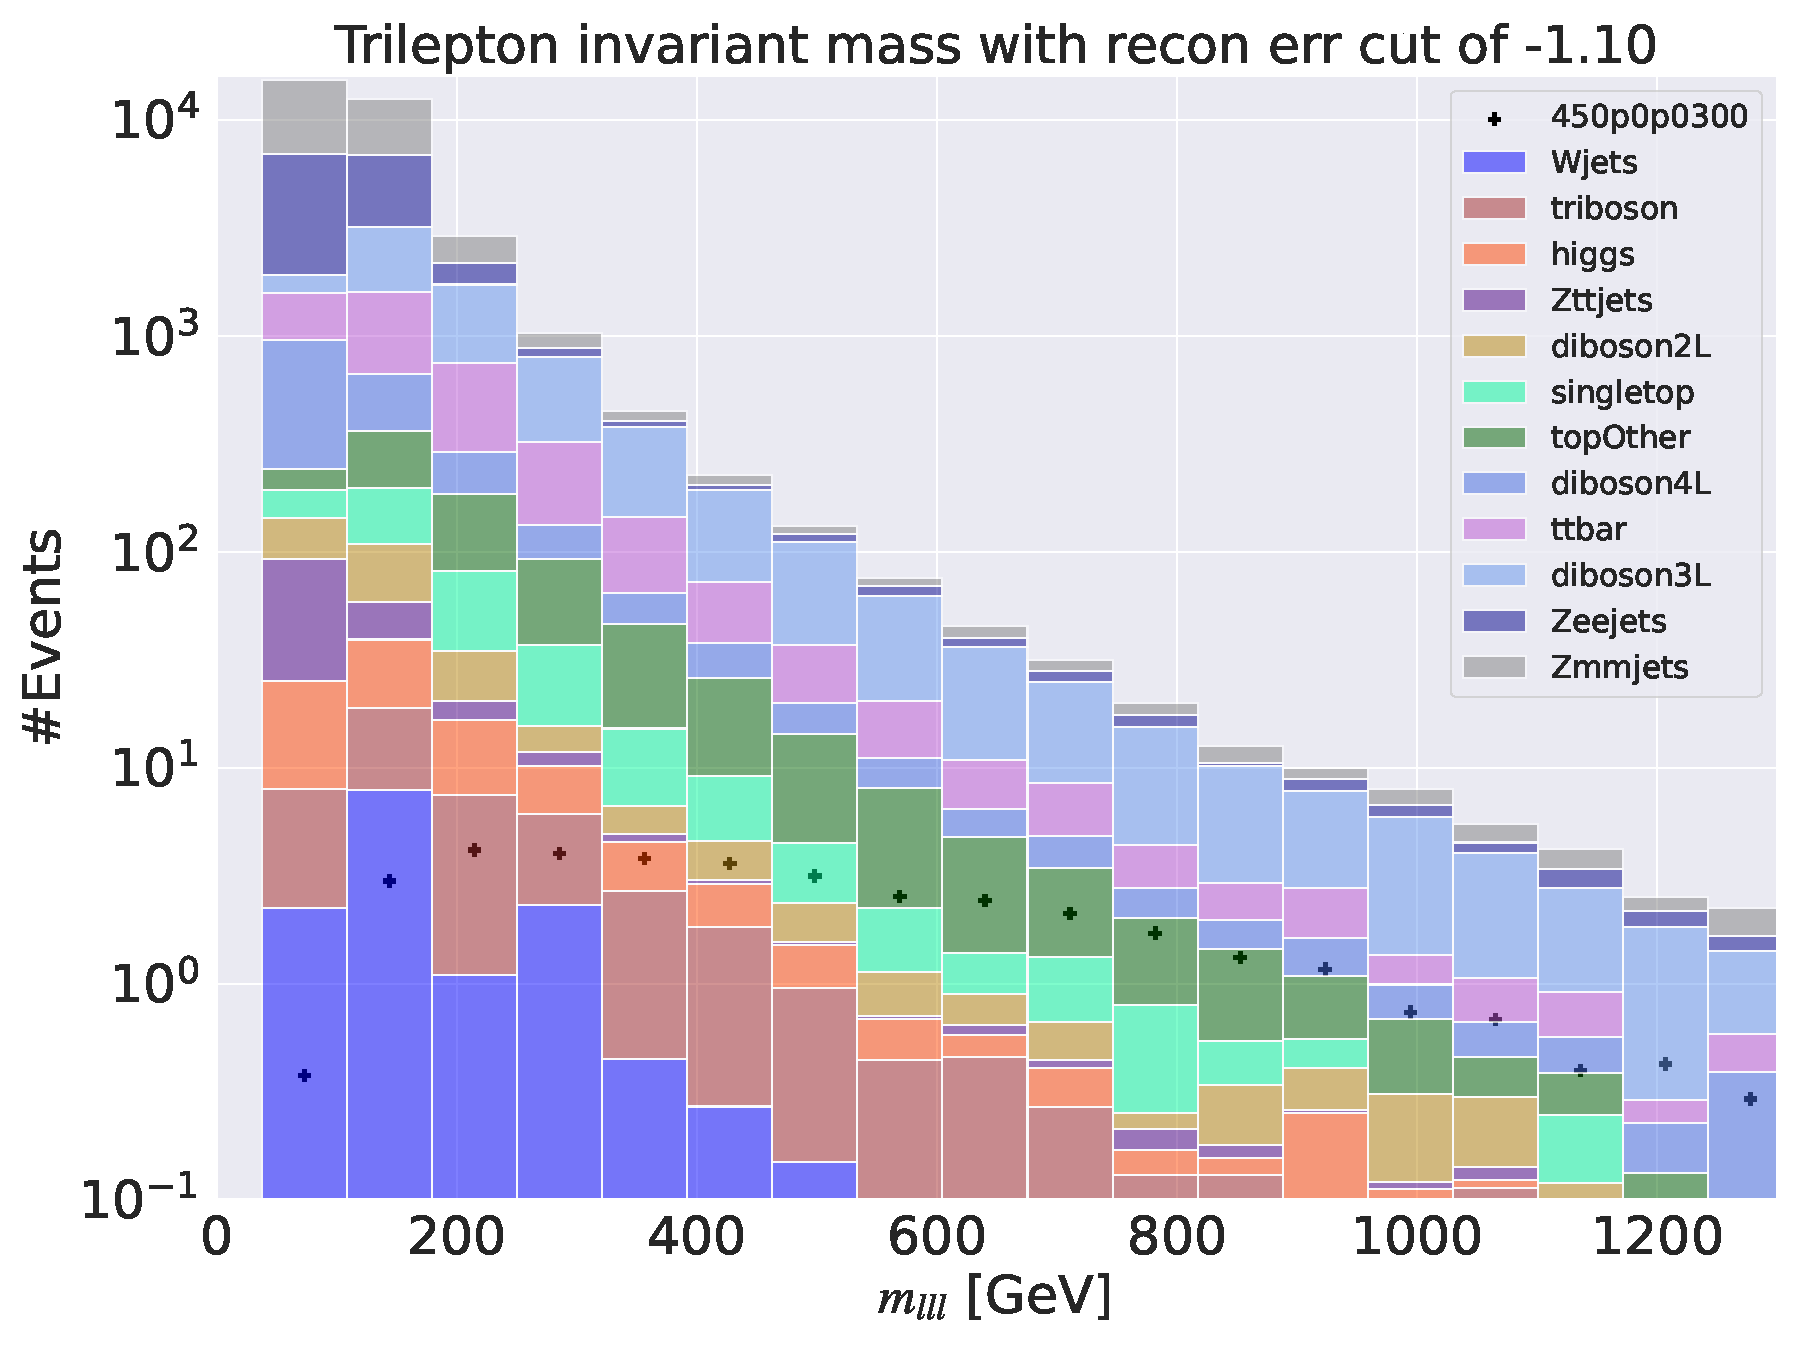
\includegraphics[width=\textwidth]{Figures/VAE_testing/big/3lep/b_data_recon_big_rm3_feats_sig_450p0p0300_mlll_recon_errcut_-1.10.pdf}
        \caption{}
        \label{fig:VAE_3lep_big_mlll_450}
    \end{subfigure}
    \hfill   
    \begin{subfigure}{.49\textwidth}
        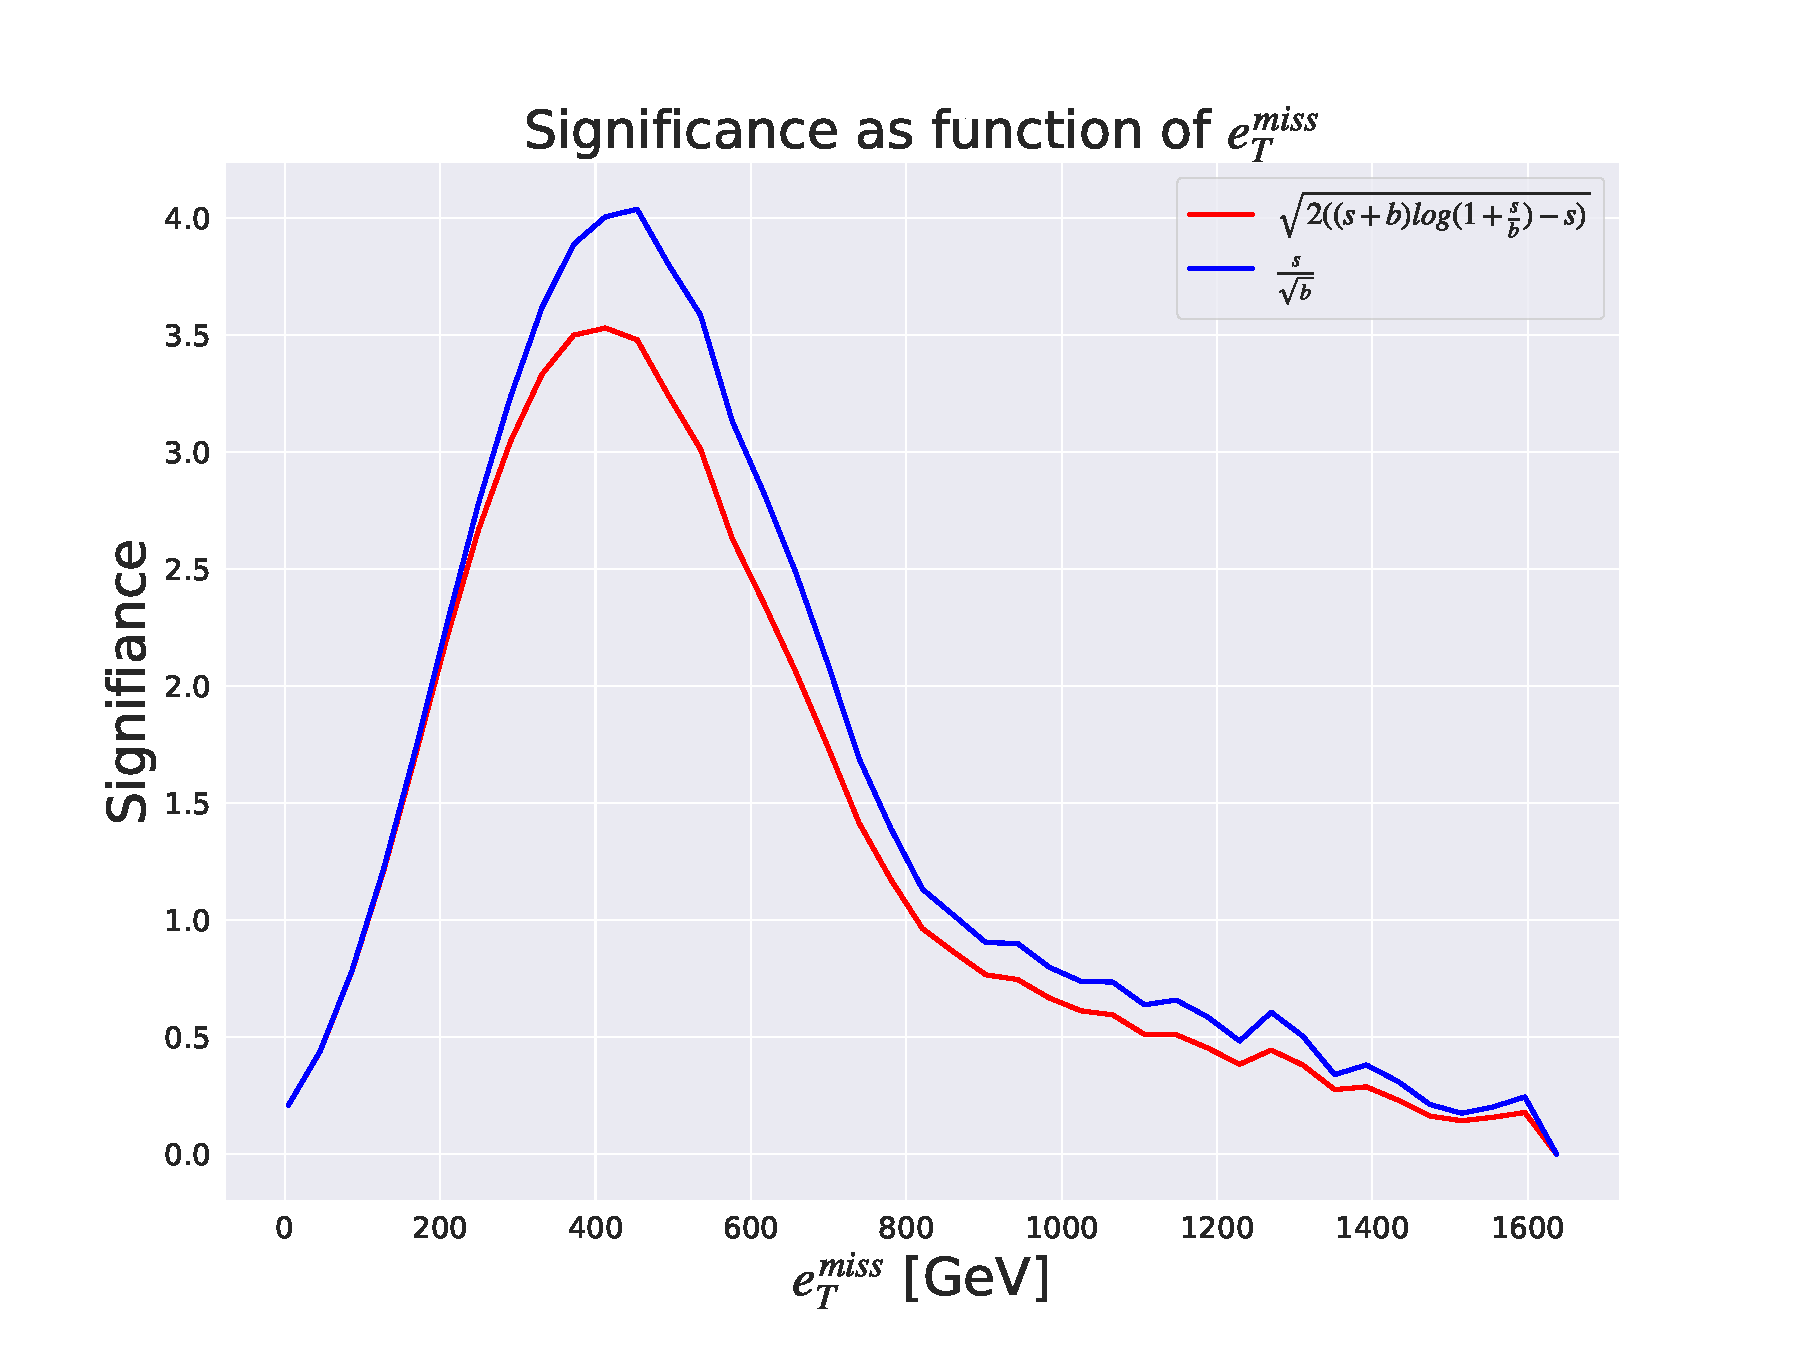
\includegraphics[width=\textwidth]{Figures/VAE_testing/big/3lep/significance_etmiss_450p0p0300_-1.0969148715571329.pdf}
        \caption{}
        \label{fig:VAE_3lep_big_signi_450}
    \end{subfigure}
    \hfill      
    \caption[3lep deep network | $450p300$ | VAE]{Reconstruction error, $e_T^{miss}$ signal region, $m_{lll}$ signal region and significance as function of 
    $e_T^{miss}$ for the deep variational autoencoder using the SUSY $450p300$.}
    \label{fig:VAE_3lep_big_rec_sig_signi_450}
\end{figure}

\begin{figure}[H]
    \centering
    \begin{subfigure}{.49\textwidth}
        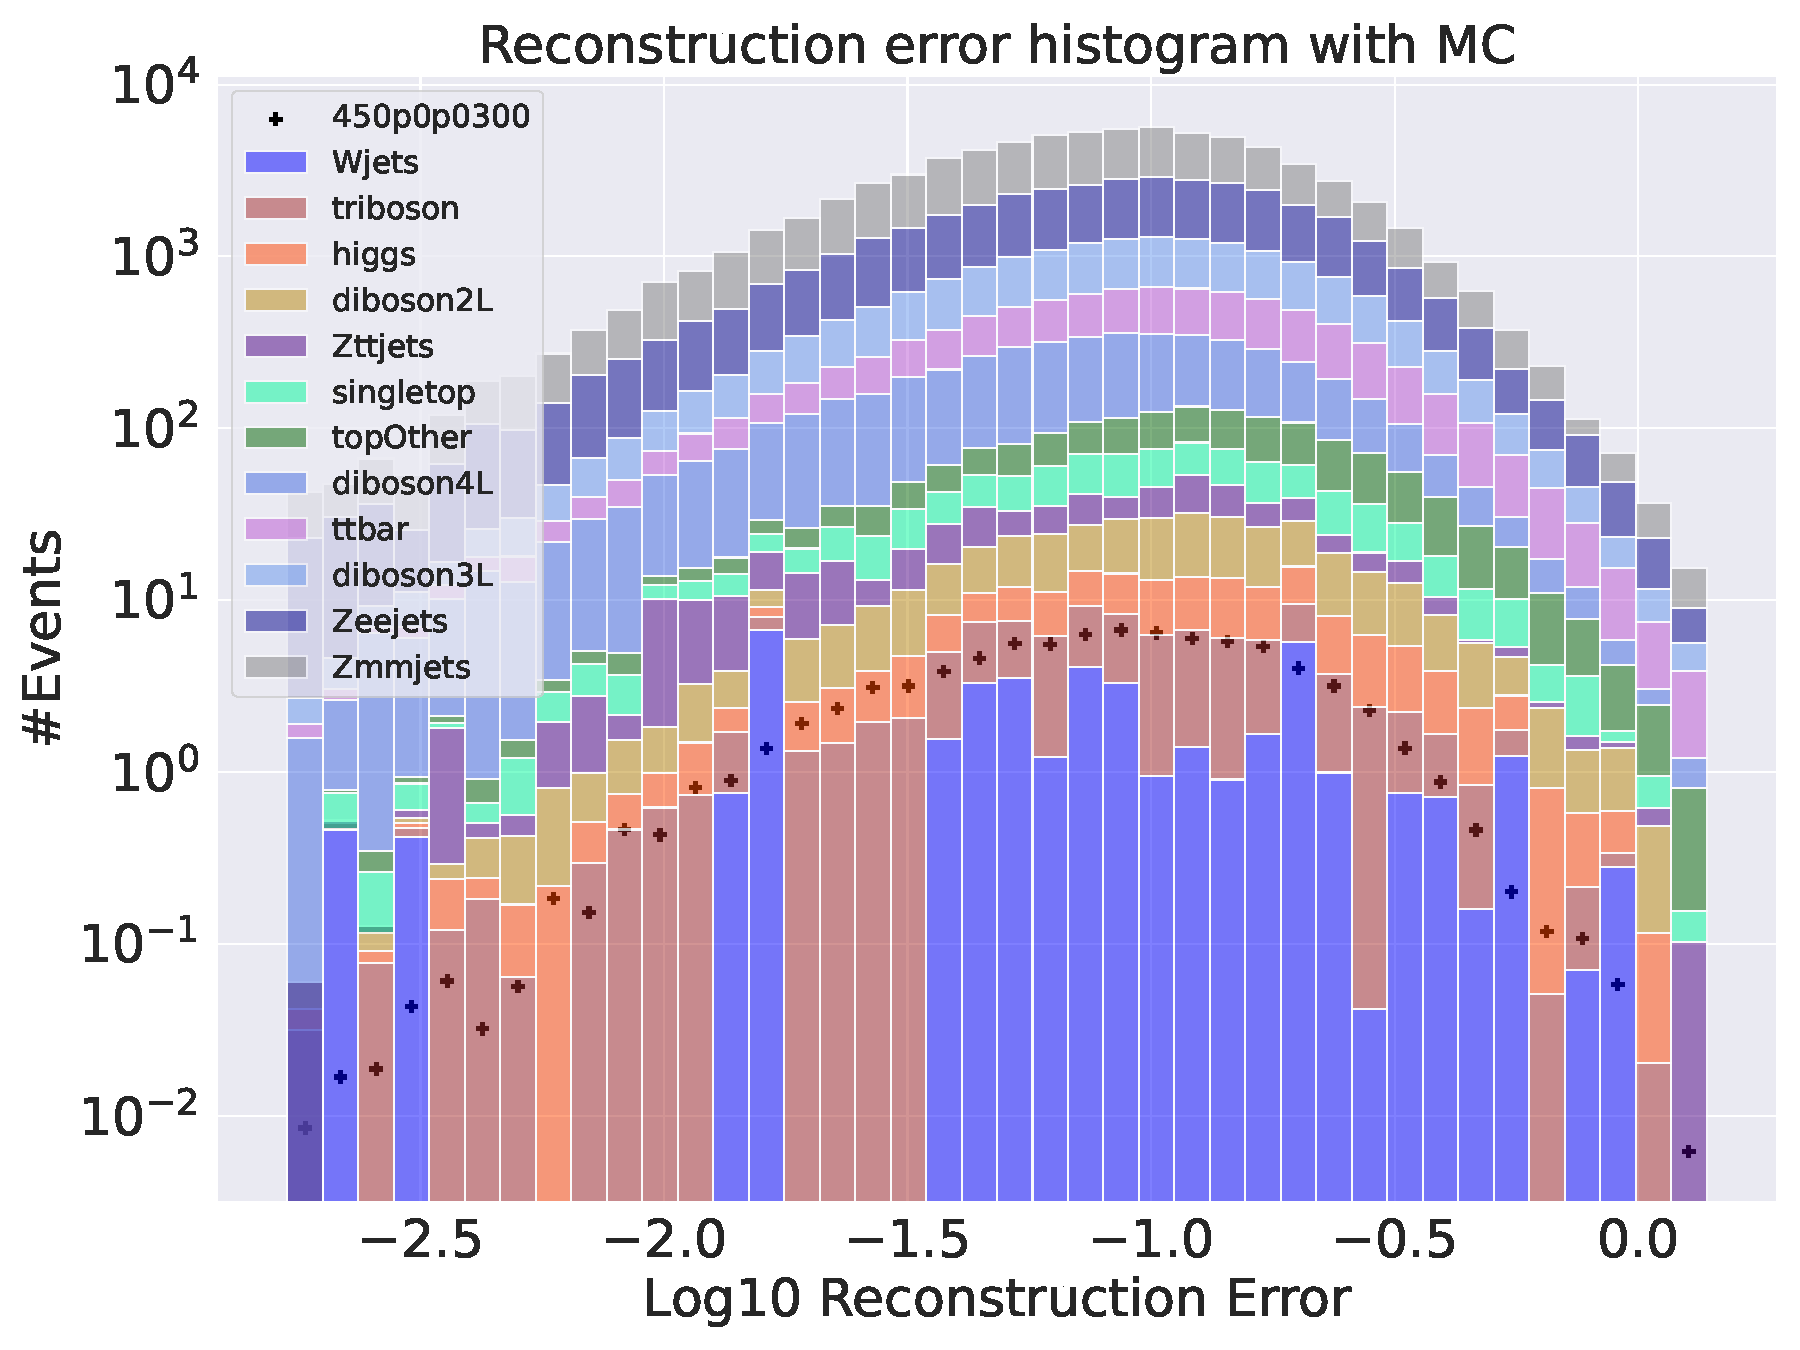
\includegraphics[width=\textwidth]{Figures/VAE_testing/small/3lep/b_data_recon_big_rm3_feats_sig_450p0p0300.pdf}
        \caption{ }
        \label{fig:VAE_3lep_small_450}
    \end{subfigure}
    \hfill
    \begin{subfigure}{.49\textwidth}
        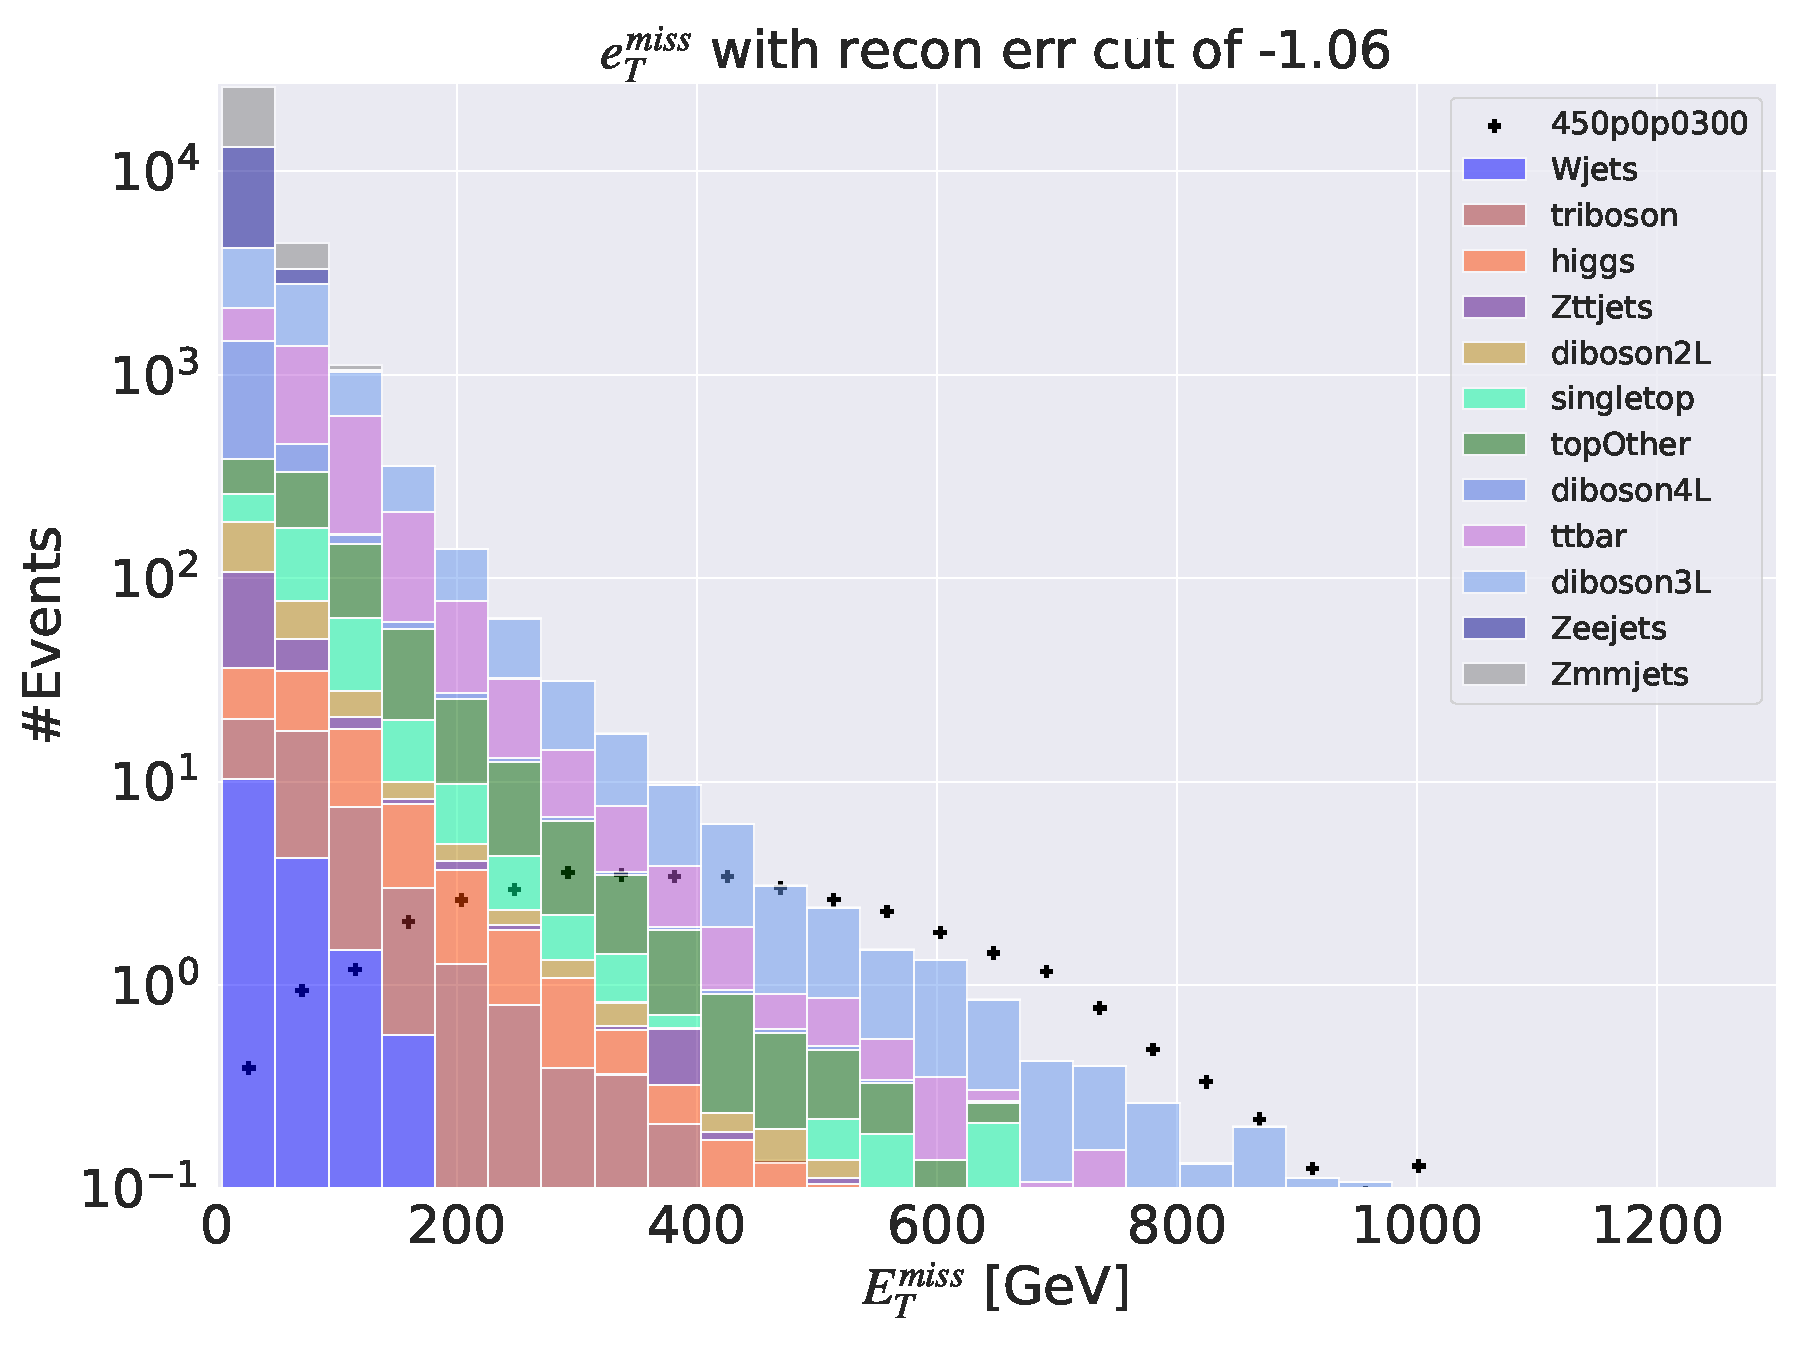
\includegraphics[width=\textwidth]{Figures/VAE_testing/small/3lep/b_data_recon_big_rm3_feats_sig_450p0p0300_etmiss_recon_errcut_-1.06.pdf}
        \caption{}
        \label{fig:VAE_3lep_small_etmiss_450}
    \end{subfigure}
    \hfill
    \begin{subfigure}{.49\textwidth}
        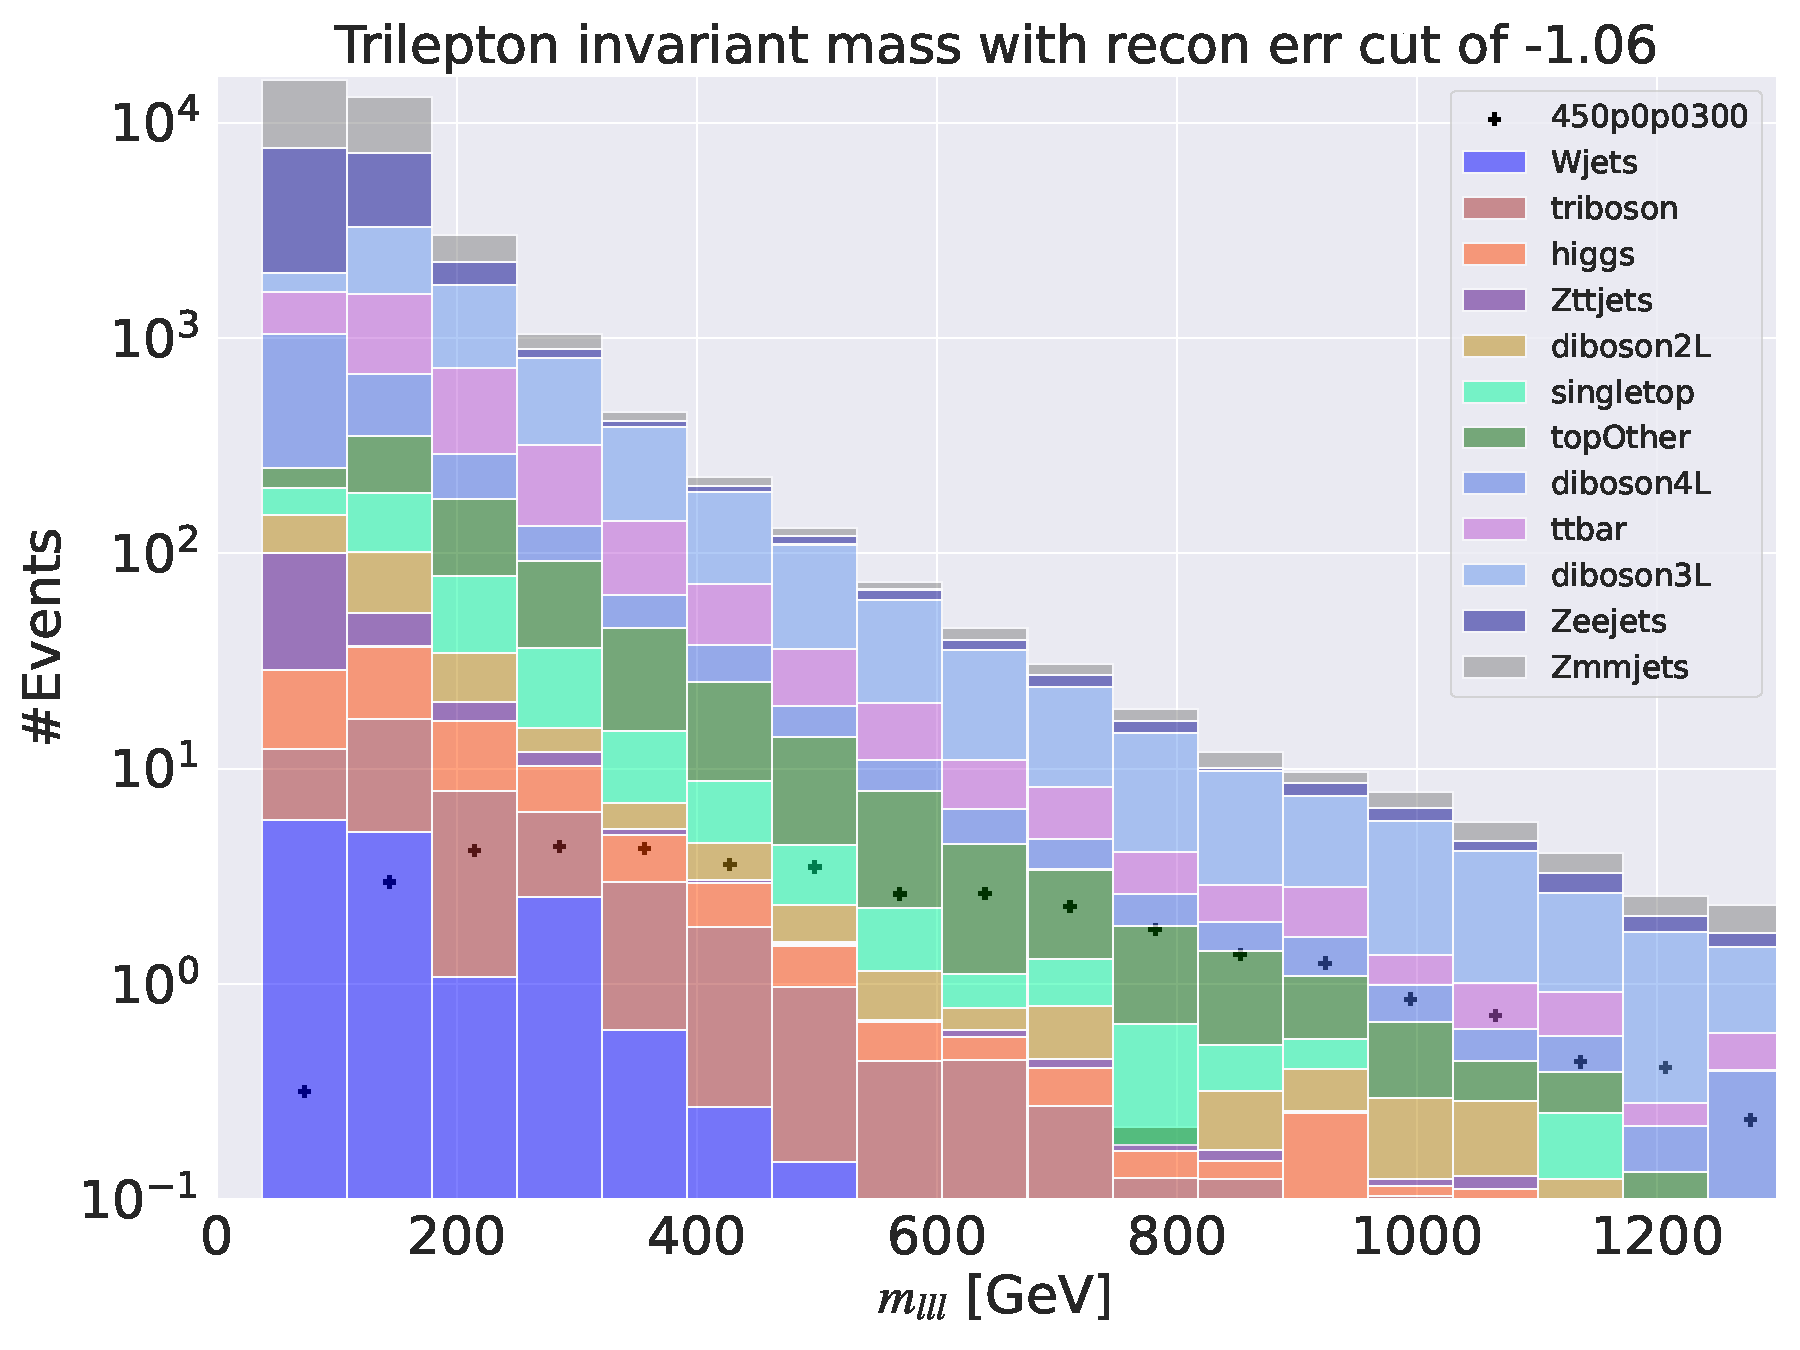
\includegraphics[width=\textwidth]{Figures/VAE_testing/small/3lep/b_data_recon_big_rm3_feats_sig_450p0p0300_mlll_recon_errcut_-1.06.pdf}
        \caption{}
        \label{fig:VAE_3lep_small_mlll_450}
    \end{subfigure}
    \hfill   
    \begin{subfigure}{.49\textwidth}
        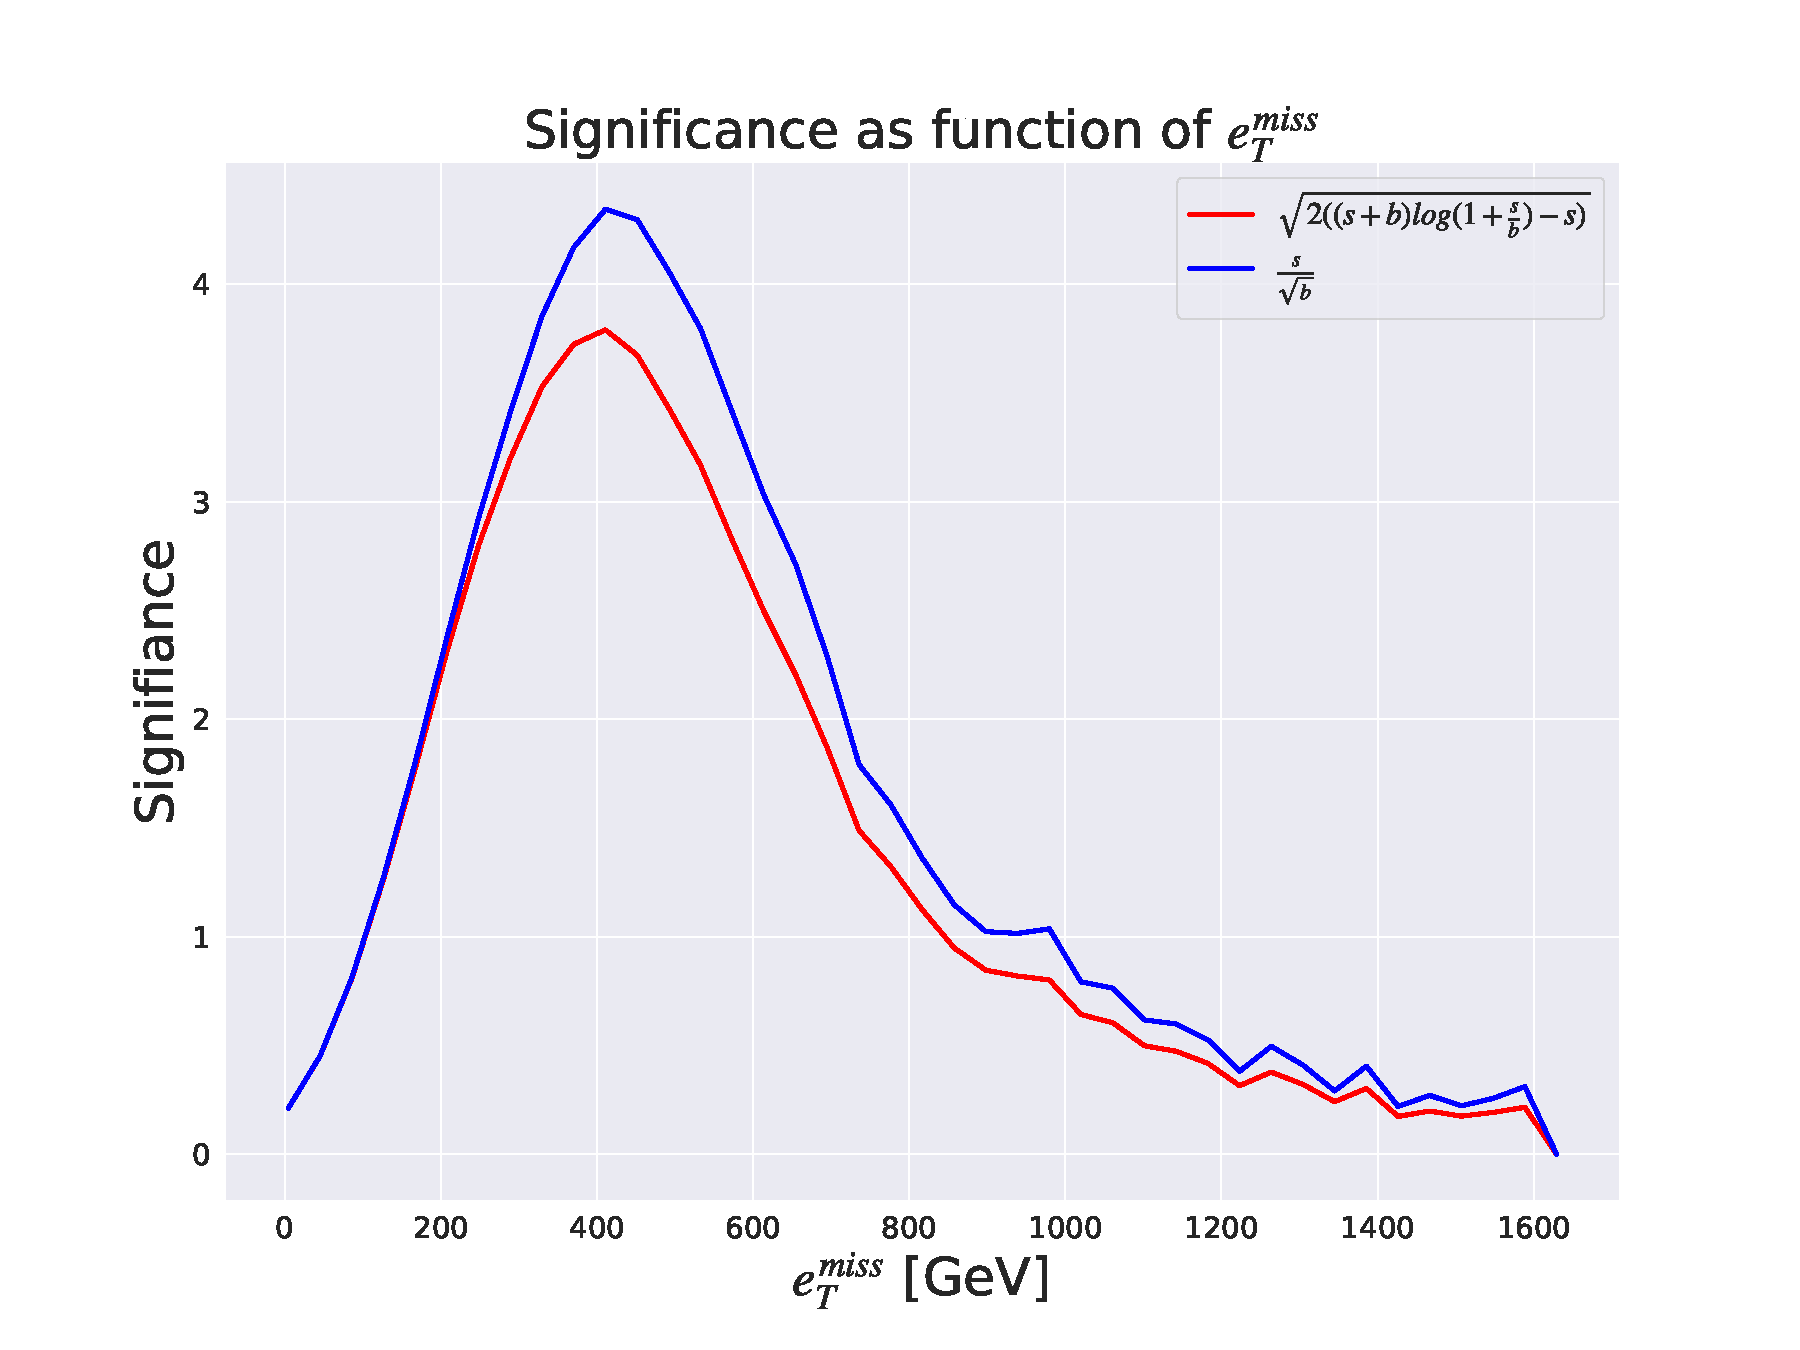
\includegraphics[width=\textwidth]{Figures/VAE_testing/small/3lep/significance_etmiss_450p0p0300_-1.0610372272331543.pdf}
        \caption{}
        \label{fig:VAE_3lep_small_signi_450}
    \end{subfigure}
    \hfill      
    \caption[3lep shallow network | $450p300$ | VAE]{Reconstruction error, $e_T^{miss}$ signal region, $m_{lll}$ signal region and significance as function of 
    $e_T^{miss}$ for the shallow variational autoencoder using the SUSY $450p300$.}
    \label{fig:VAE_3lep_small_rec_sig_signi_450}
\end{figure}








\begin{figure}[H]
    \centering
    \begin{subfigure}{.49\textwidth}
        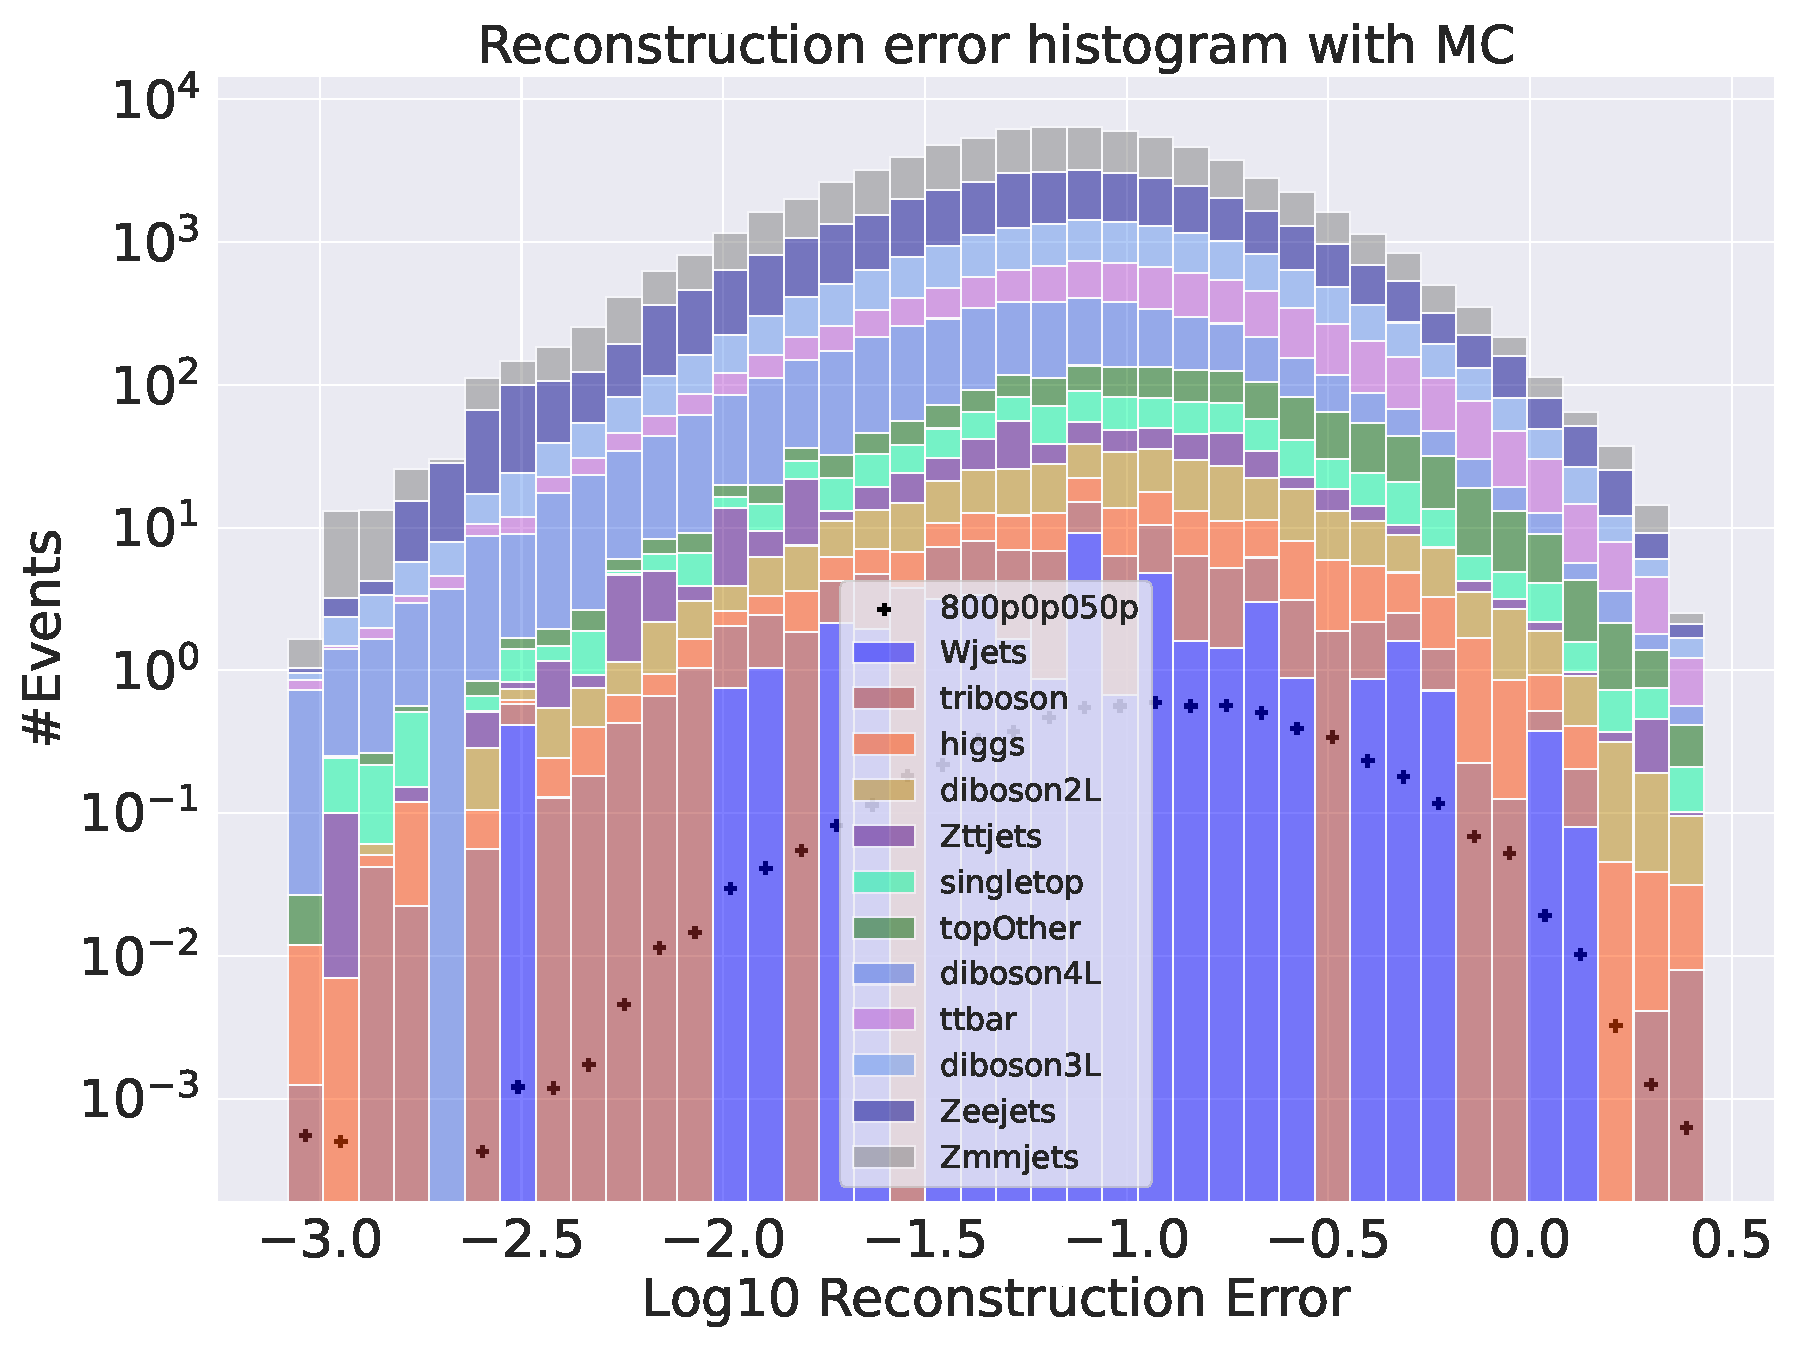
\includegraphics[width=\textwidth]{Figures/VAE_testing/big/3lep/b_data_recon_big_rm3_feats_sig_800p0p050p.pdf}
        \caption{ }
        \label{fig:VAE_3lep_big_800}
    \end{subfigure}
    \hfill
    \begin{subfigure}{.49\textwidth}
        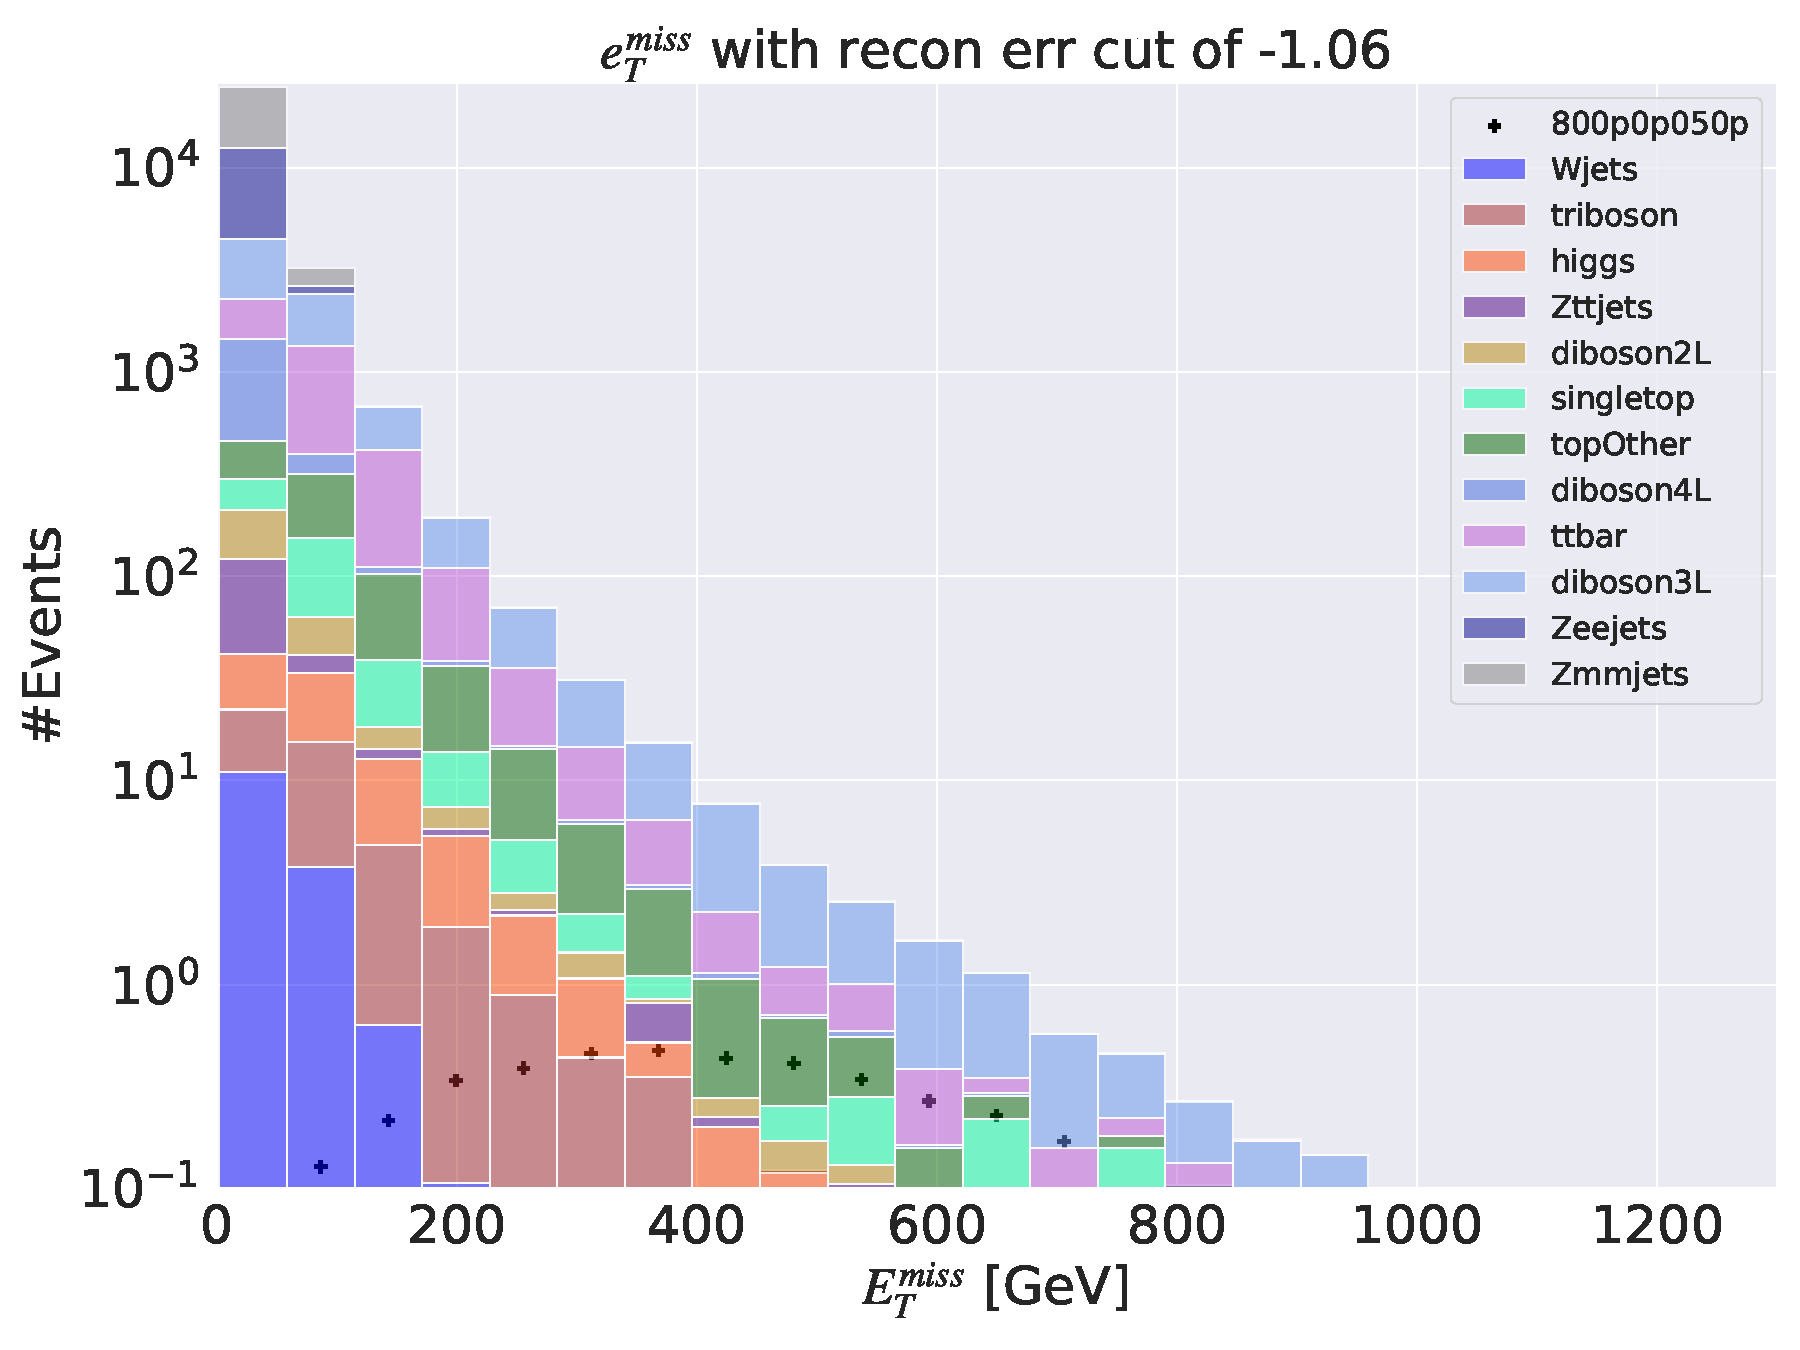
\includegraphics[width=\textwidth]{Figures/VAE_testing/big/3lep/b_data_recon_big_rm3_feats_sig_800p0p050p_etmiss_recon_errcut_-1.06.pdf}
        \caption{}
        \label{fig:VAE_3lep_big_etmiss_800}
    \end{subfigure}
    \hfill
    \begin{subfigure}{.49\textwidth}
        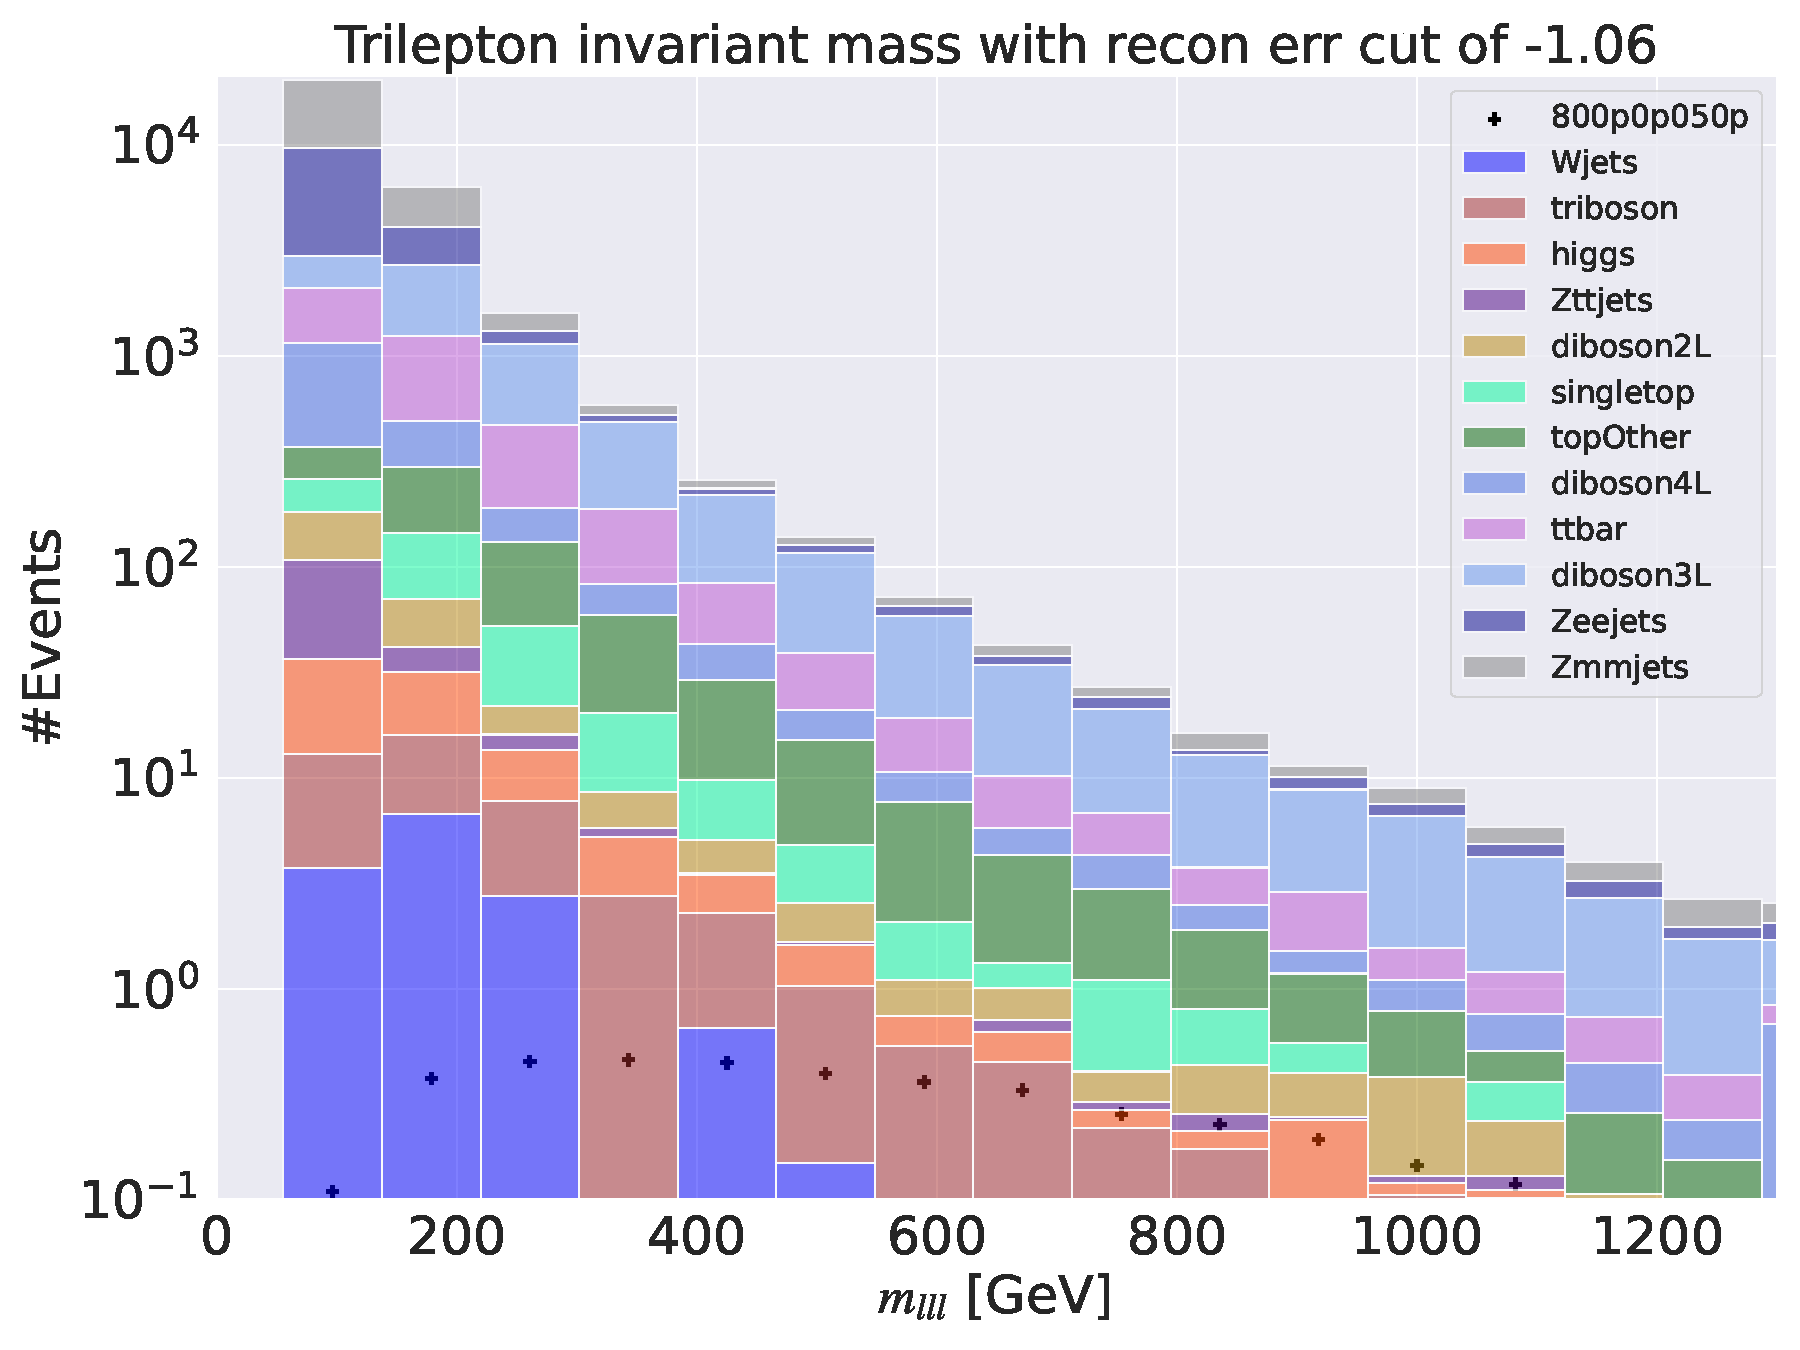
\includegraphics[width=\textwidth]{Figures/VAE_testing/big/3lep/b_data_recon_big_rm3_feats_sig_800p0p050p_mlll_recon_errcut_-1.06.pdf}
        \caption{}
        \label{fig:VAE_3lep_big_mlll_800}
    \end{subfigure}
    \hfill   
    \begin{subfigure}{.49\textwidth}
        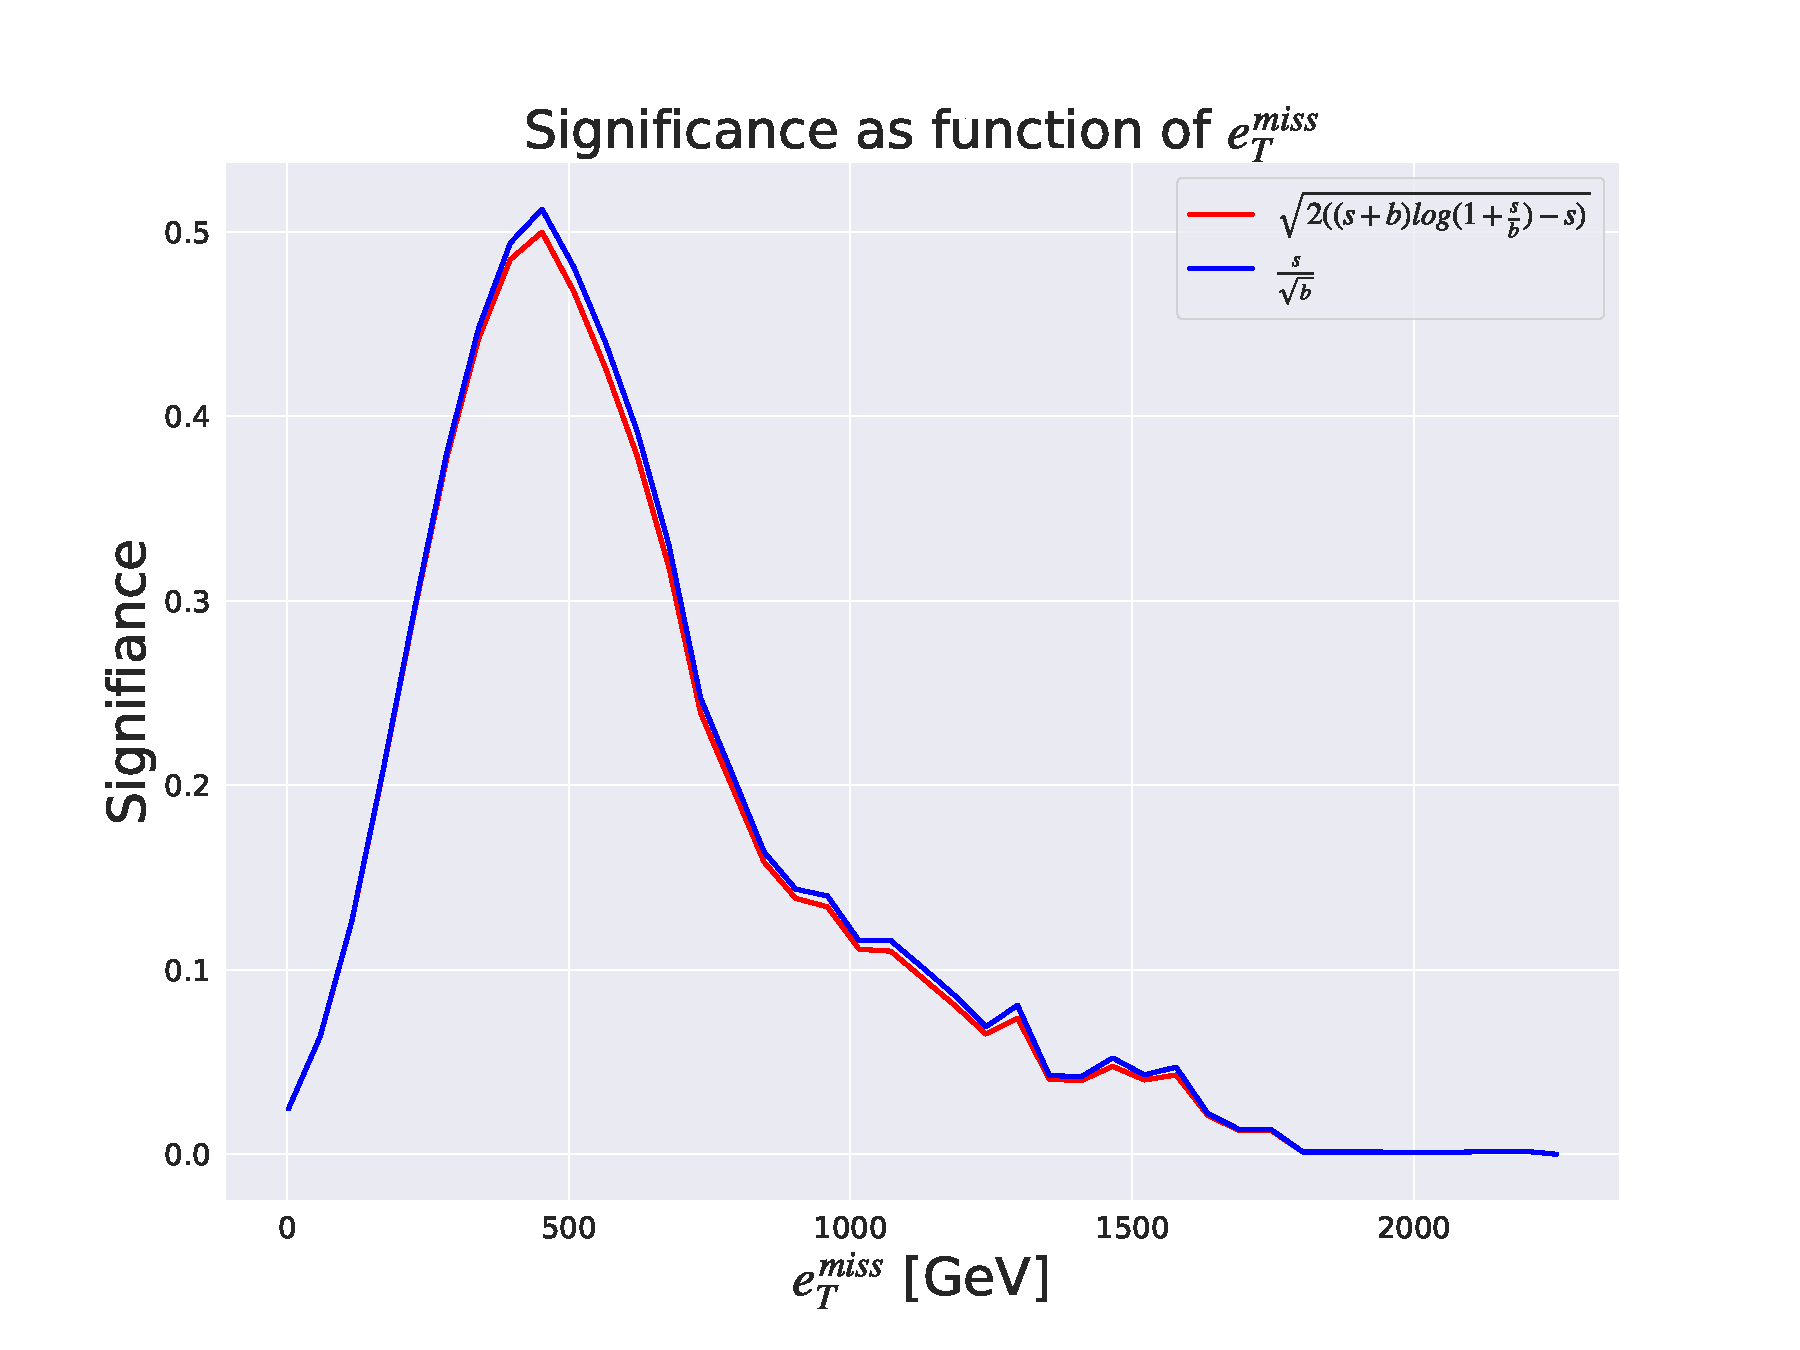
\includegraphics[width=\textwidth]{Figures/VAE_testing/big/3lep/significance_etmiss_800p0p050p_-1.0588523538160817.pdf}
        \caption{}
        \label{fig:VAE_3lep_big_signi_800}
    \end{subfigure}
    \hfill      
    \caption[3lep deep network | $800p50$ | VAE]{Reconstruction error, $e_T^{miss}$ signal region, $m_{lll}$ signal region and significance as function of 
    $e_T^{miss}$ for the deep variational autoencoder using the SUSY $800p50$.}
    \label{fig:VAE_3lep_big_rec_sig_signi_800}
\end{figure}

\begin{figure}[H]
    \centering
    \begin{subfigure}{.49\textwidth}
        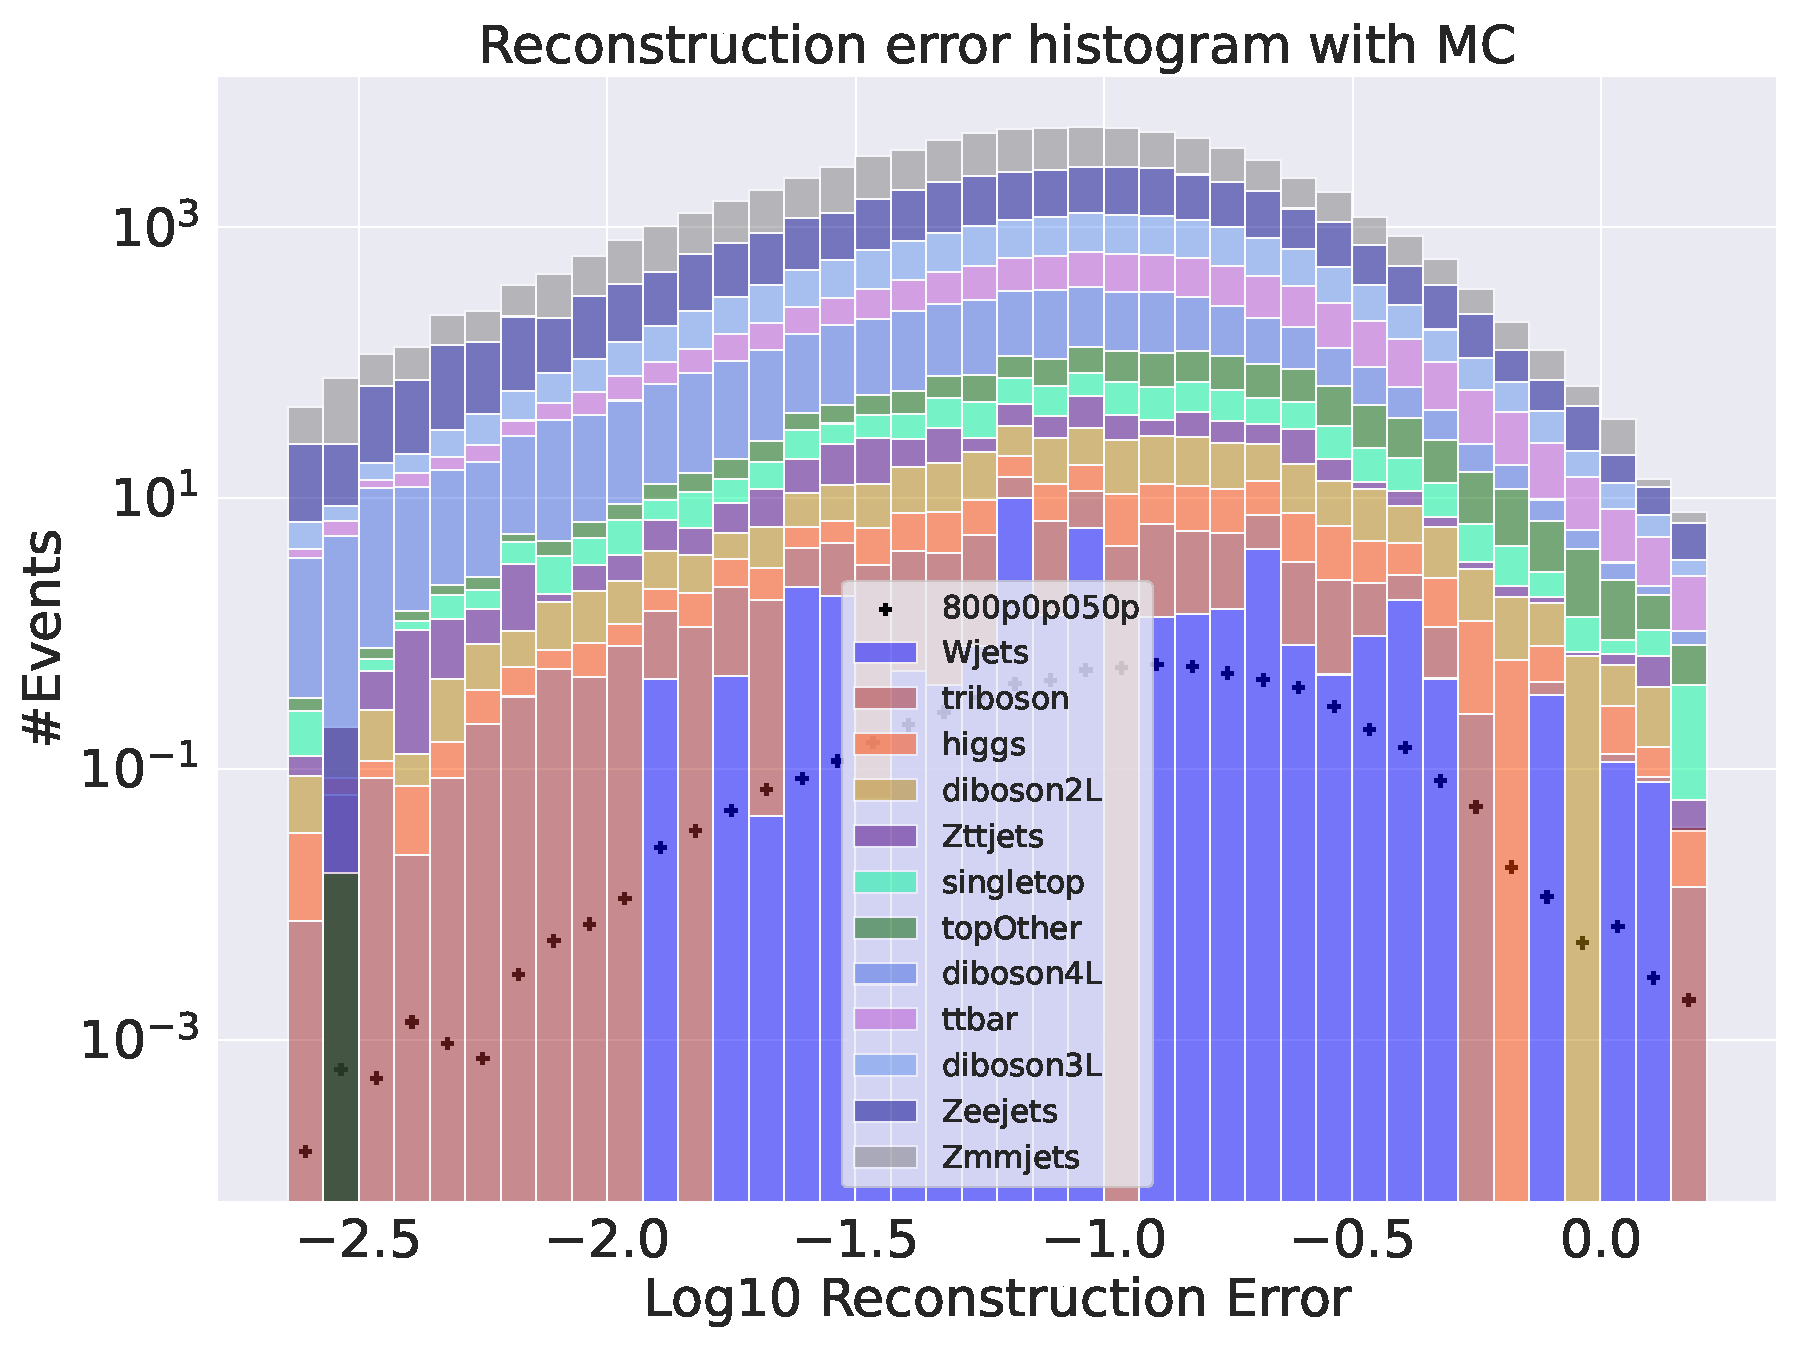
\includegraphics[width=\textwidth]{Figures/VAE_testing/small/3lep/b_data_recon_big_rm3_feats_sig_800p0p050p.pdf}
        \caption{ }
        \label{fig:VAE_3lep_small_800}
    \end{subfigure}
    \hfill
    \begin{subfigure}{.49\textwidth}
        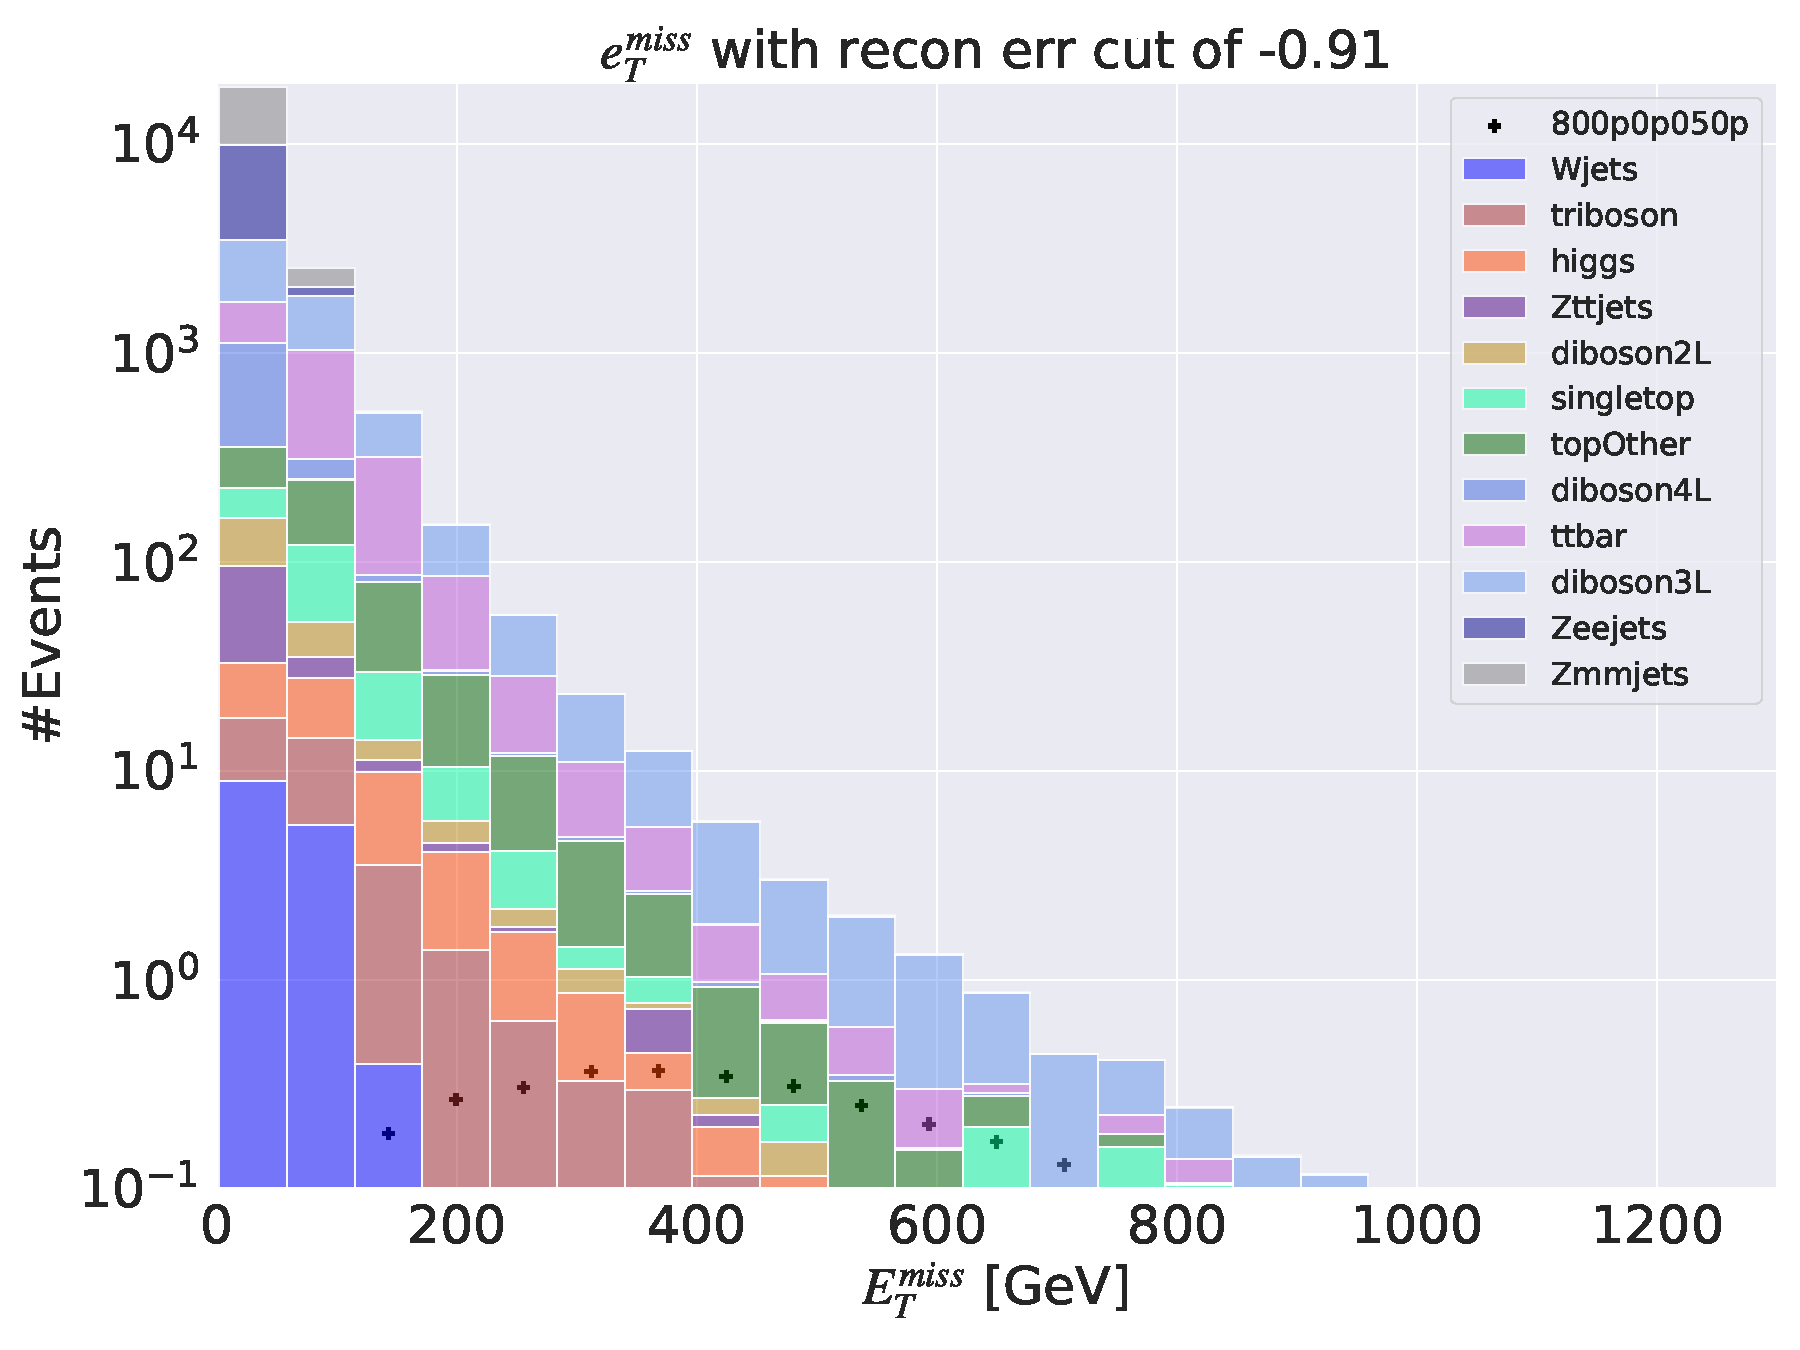
\includegraphics[width=\textwidth]{Figures/VAE_testing/small/3lep/b_data_recon_big_rm3_feats_sig_800p0p050p_etmiss_recon_errcut_-0.91.pdf}
        \caption{}
        \label{fig:VAE_3lep_small_etmiss_800}
    \end{subfigure}
    \hfill
    \begin{subfigure}{.49\textwidth}
        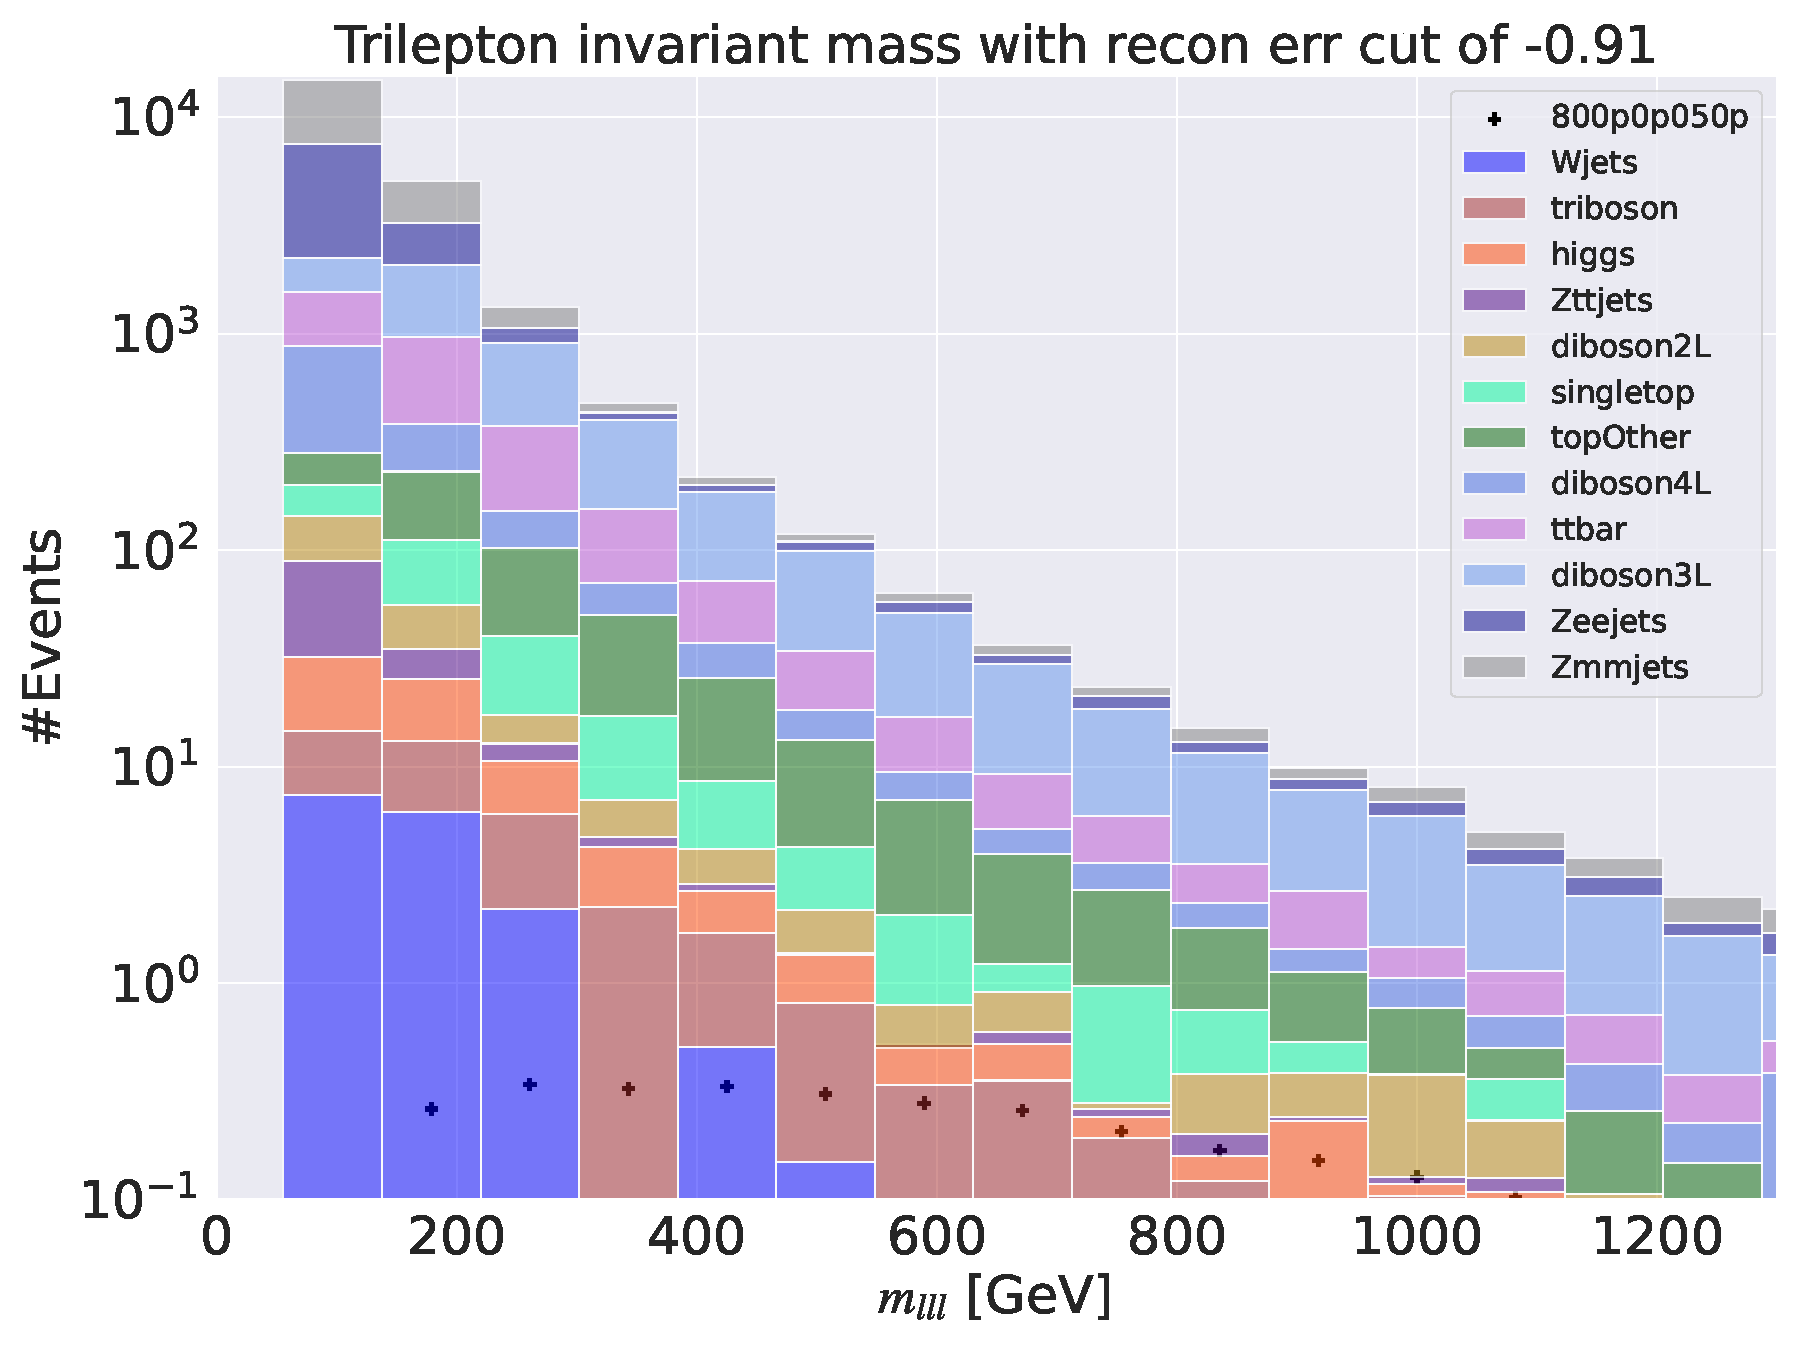
\includegraphics[width=\textwidth]{Figures/VAE_testing/small/3lep/b_data_recon_big_rm3_feats_sig_800p0p050p_mlll_recon_errcut_-0.91.pdf}
        \caption{}
        \label{fig:VAE_3lep_small_mlll_800}
    \end{subfigure}
    \hfill   
    \begin{subfigure}{.49\textwidth}
        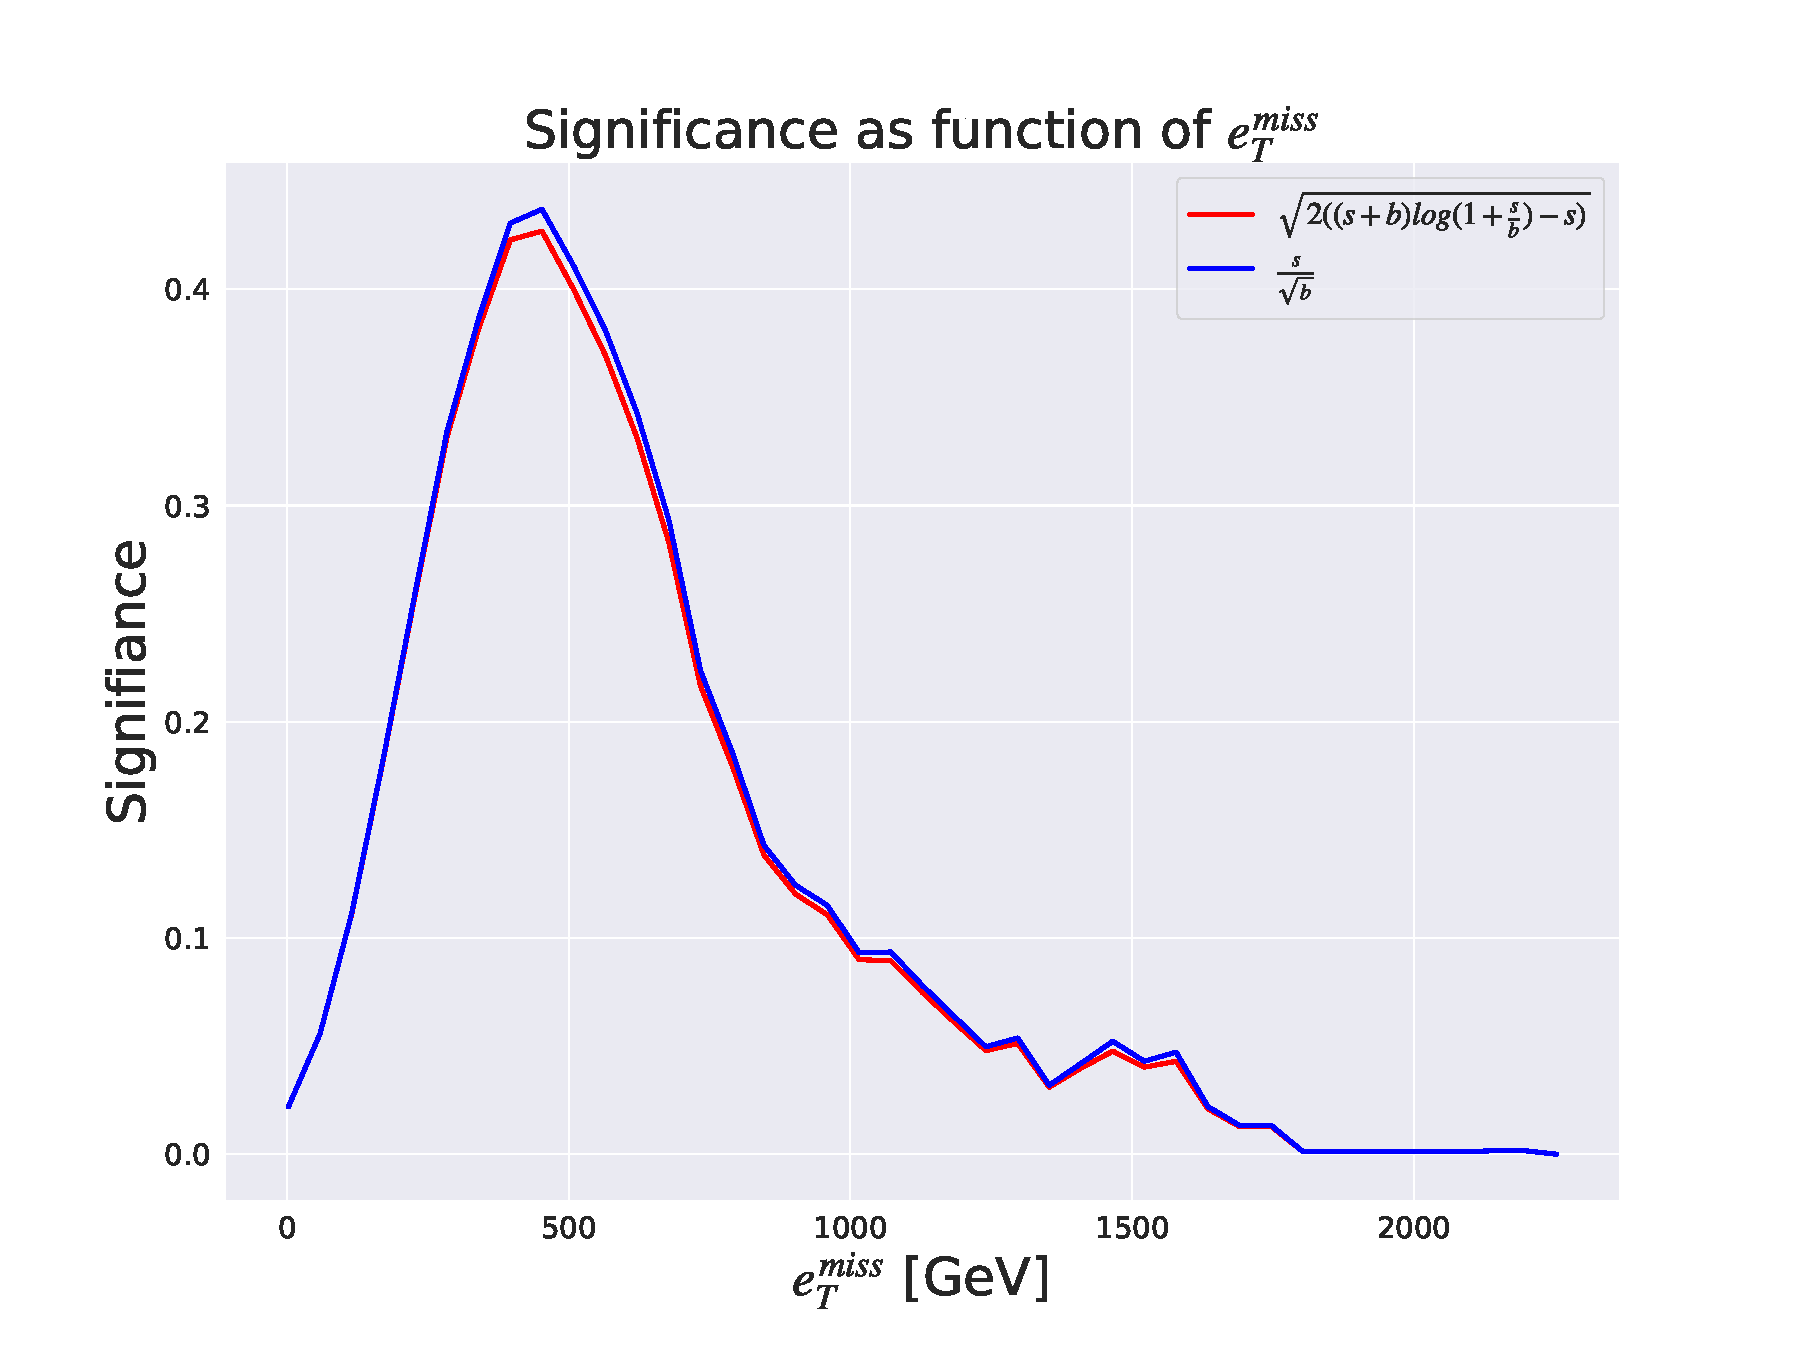
\includegraphics[width=\textwidth]{Figures/VAE_testing/small/3lep/significance_etmiss_800p0p050p_-0.9142561918890106.pdf}
        \caption{}
        \label{fig:VAE_3lep_small_signi_800}
    \end{subfigure}
    \hfill      
    \caption[3lep shallow network | $800p50$ | VAE]{Reconstruction error, $e_T^{miss}$ signal region, $m_{lll}$ signal region and significance as function of 
    $e_T^{miss}$ for the shallow variational autoencoder using the SUSY $800p50$.}
    \label{fig:VAE_3lep_small_rec_sig_signi_800}
\end{figure}


In figures \ref{fig:VAE_3lep_big_rec_sig_signi_450}, \ref{fig:VAE_3lep_small_rec_sig_signi_450}, 
\ref{fig:VAE_3lep_big_rec_sig_signi_800} and \ref{fig:VAE_3lep_small_rec_sig_signi_800} we have four 
subplots containing the total reconstruction error distributions, the $e_T^{miss}$ signal region, 
the $m_{lll}$ signal region and the significance as function of $e_T^{miss}$ curve respectively for 
the shallow and deep variational autoencoder. From figures \ref{fig:VAE_3lep_big_450}, \ref{fig:VAE_3lep_small_450},
\ref{fig:VAE_3lep_big_800}, \ref{fig:VAE_3lep_small_800} we observe that the variational 
autoencoder seems to struggle with differentiating between background and signal, having the 
two distributions laying on top of each other. There is however a slight difference in the 
shape of the distributions from the shallow and deep network. The shallow has a more narrow 
and slightly more left leaning shape, whereas the deep network has a slightly more broad 
distribution shifted a bit to the right. The bulk of the events are between $10^{-2}$ and $10^{-0.5}$ 
reconstruction error, indicating that the autoencoder struggles to learn  the internal RMM 
structures for the 3 lepton + $e_T^{miss}$ final state MC. The somewhat Gaussian distribution 
differs between the two SUSY samples. As the networks were retrained each time, it could indicate 
that the distribution in part is due to the sampling in the latent space. \par 

In figures \ref{fig:VAE_3lep_big_etmiss_450}, \ref{fig:VAE_3lep_small_etmiss_450}, 
\ref{fig:VAE_3lep_big_etmiss_800} and  \ref{fig:VAE_3lep_small_etmiss_800} we have the 
reconstruction error cut imposed on the SM MC and the signal samples. Interestingly, one should 
note that although the total reconstruction error distributions are not well separated, the 
signal regions show a separation in distribution peaks. Now, unlike in the regular autoencoder 
case, the variational autoencoder allows for almost two orders of magnitude more background 
events in the signal region. \marginpar{Rar setning} This is because of the algorithm used to determine the 
reconstruction error cut by means of finding the median and iteratively increasing the criterion. 
Because the two distributions are on top of each other, we get a lot of background events, 
but we also get the peak of the signal distributions, which is why we see the clear 
separation in the figures \ref{fig:VAE_3lep_big_etmiss_450}, \ref{fig:VAE_3lep_small_etmiss_450}, 
\ref{fig:VAE_3lep_big_etmiss_800} and \ref{fig:VAE_3lep_small_etmiss_800}. \par 

In figures \ref{fig:VAE_3lep_big_mlll_450}, \ref{fig:VAE_3lep_small_mlll_450}, 
\ref{fig:VAE_3lep_big_mlll_800} and  \ref{fig:VAE_3lep_small_mlll_800} we have the signal 
region in the $m_{lll}$ feature. Here, as with the $e_T^{miss}$ distribution, the least 
strict reconstruction error cut has been imposed on the region. There are little to no separation between the peaks 
to observe. \par 

In figures \ref{fig:VAE_3lep_big_signi_450}, \ref{fig:VAE_3lep_small_signi_450}, \ref{fig:VAE_3lep_big_signi_800} and  
\ref{fig:VAE_3lep_small_signi_800} we have the significance as a function of the $e_T^{miss}$.
Interestingly, for the SUSY $450p300$ case, we have that both the deep and shallow 
autoencoder manages to get a significance of around 4, which is much better than the 
regular autoencoder which got around 0.7. Likewise for the other SUSY signal, but 
here the difference was small. From these figures a further cut on the 
$e_T^{miss}$ on around 400 GeV provides the best significance. Also note the tails of 
the significance figures, as they all contain little background and or signal and are 
thus not of interest. 


